%
% @author  unknown
% @version 1.1a
% @edit by Andreas Febrian
% @edit by Moeljono Widjaja
% @edit by Arya Wicaksana
%
% Template Laporan Skripsi Informatika UMN
%

%
% Tipe dokumen adalah report dengan satu kolom. 
%
\documentclass[12pt, a4paper, onecolumn, oneside, final]{report1}

% \usepackage{indentfirst}

% Load konfigurasi LaTeX untuk tipe laporan thesis
\usepackage{_internals/umnthesis}
\usepackage{algorithm}
\usepackage{algorithmic}
\usepackage{amsmath}
\usepackage{amsfonts}
\usepackage{float}
\usepackage{graphicx}
\usepackage{booktabs}

% Daftar pemenggalan suku kata dan istilah dalam LaTeX
%
% Hyphenation untuk Indonesia 
%
% @author  Andreas Febrian
% @version 1.00
% 
% Tambahkan cara pemenggalan kata-kata yang salah dipenggal secara otomatis 
% oleh LaTeX. Jika kata tersebut dapat dipenggal dengan benar, maka tidak 
% perlu ditambahkan dalam berkas ini. Tanda pemenggalan kata menggunakan 
% tanda '-'; contoh:
% menarik
%   --> pemenggalan: me-na-rik
%

\hyphenation{
    % alphabhet A
    a-na-li-sa a-tur 
    a-pli-ka-si 
    % alphabhet B
    ba-ngun-an 
    be-be-ra-pa 
    ber-ge-rak
    ber-ke-lan-jut-an 
    ber-pe-nga-ruh 
    % alphabhet C
    ca-ri
    % alphabhet D
    di-sim-pan di-pim-pin de-ngan da-e-rah di-ba-ngun da-pat di-nya-ta-kan 
    di-sim-bol-kan di-pi-lih di-li-hat de-fi-ni-si
    % alphabhet E
    e-ner-gi eks-klu-sif
    % alphabhet F
    fa-si-li-tas
    % alphabhet G
    ga-bung-an ge-rak
    % alphabhet H
    ha-lang-an
    % alphabhet I
    % alphabhet J
    % alphabhet K
    ke-hi-lang-an
    ku-ning 
    kua-li-tas ka-me-ra ke-mung-kin-an ke-se-pa-ham-an
    % alphabhet L
    ling-kung-an
    % alphabhet M
    me-neng-ah
    meng-a-tas-i me-mung-kin-kan me-nge-na-i me-ngi-rim-kan 
    meng-u-bah meng-a-dap-ta-si me-nya-ta-kan mo-di-fi-ka-si
    meng-a-tur
    % alphabhet N
    nya-ta non-eks-klu-sif
    % alphabhet O
    % alphabhet P
	pe-nye-rap-an 
	pe-ngon-trol
    pe-mo-del-an
    pe-ran  pe-ran-an-nya
    pem-ba-ngun-an pre-si-den pe-me-rin-tah prio-ri-tas peng-am-bil-an 
    peng-ga-bung-an pe-nga-was-an pe-ngem-bang-an 
    pe-nga-ruh pa-ra-lel-is-me per-hi-tung-an per-ma-sa-lah-an 
    pen-ca-ri-an peng-struk-tur-an
    % alphabhet Q
    % alphabhet R
    ran-cang-an
    % alphabhet S
    si-mu-la-si sa-ngat
    % alphabhet T
    te-ngah
    ter-da-pat
    % alphabhet U
    % alphabhet V
    % alphabhet W
    % alphabhet X
    % alphabhet Y
    % alphabhet Z
    % special
}

% Load konfigurasi khusus untuk laporan yang sedang dibuat
%-----------------------------------------------------------------------------%
% Informasi Mengenai Dokumen
%-----------------------------------------------------------------------------%
% 
% Judul laporan. 
\var{\judul}{Klasifikasi Deepfake Pada Gambar Wajah Menggunakan Ensemble Deep Learning Dengan Pendekatan Weight Loss Averaging}
% Judul Pendek (Tiga Kata Pertama). 
\var{\judulPendek}{Klasifikasi Deepfake Pada}
% 
% Tulis kembali judul laporan, kali ini akan diubah menjadi huruf kapital
\Var{\Judul}{Klasifikasi Deepfake Pada Gambar Wajah Menggunakan Ensemble Deep Learning Dengan Pendekatan Weight Loss Averaging}
% 
% Tulis kembali judul laporan namun dengan bahasa Ingris (gunakan huruf KAPITAL)
\var{\JudulInggris}{Classification of Deepfakes in Facial Images Using Deep Learning Ensemble with Weight Loss Averaging Approach}

% 
% Tipe laporan, dapat berisi Skripsi, Tugas Akhir, Thesis, atau Disertasi
\var{\type}{Skripsi}
% 
% Tulis kembali tipe laporan, kali ini akan diubah menjadi huruf kapital
\Var{\Type}{Skripsi}
% 
% Tulis nama penulis 
\var{\penulis}{Arvin Winardi}
% 
% Tulis kembali nama penulis, kali ini akan diubah menjadi huruf kapital
\Var{\Penulis}{Arvin Winardi}



% 
% Tulis NIM penulis
\var{\nim}{00000058607}
% 
% Tuliskan Jenjang Studi penulis (D3/S1/S2)
\Var{\Jenjang}{S1}
\var{\jenjang}{S1}
% 
% Tuliskan Fakultas dimana penulis berada
\Var{\Fakultas}{Teknik dan Informatika}
\var{\fakultas}{Teknik dan Informatika}
% 
% Tuliskan Program Studi yang diambil penulis
\Var{\Program}{INFORMATIKA}
\var{\program}{Informatika}
% 
% Tuliskan tahun publikasi laporan
\Var{\bulan}{"Bulan"}
\Var{\tahun}{2025}
% 
% Tuliskan gelar yang akan diperoleh dengan menyerahkan laporan ini
\var{\gelar}{Sarjana Ilmu Komputer}
% 
% Tuliskan tanggal pengesahan laporan
\var{\tanggalPengesahan}{Tgl. Pengesahan} 


% Tuliskan tanggal pengumpulan laporan, waktu dimana laporan diserahkan ke 
% penguji/sekretariat
\var{\tanggalPengumpulan}{26 Juni 2025} 


% Tuliskan tanggal sidang
\var{\hariTanggalSidang}{Jumat, 11 Juli 2025} 
\var{\waktuSidang}{13:00 s/d 15:00} 


% 
% Tuliskan tanggal keputusan sidang dikeluarkan dan penulis dinyatakan 
% lulus/tidak lulus
\var{\tanggalLulus}{Jumat, 11 Juli 2025}
% 


% Tuliskan Rektor UMN
\var{\rektorUMN}{ Dr. Ir. Andrey Andoko, M.Sc.}

% Tuliskan Dekan FTI
\var{\dekanFTI}{Dr.   Eng.   Niki  Prastomo,  S.T.,  M.Sc.}

% Tuliskan Kaprodi Informatika 
\var{\kaprodi}{Arya Wicaksana, S.Kom., M.Eng.Sc., OCA}
\var{\kaprodiNIDN}{ NIDN: 0315109103}

% Tuliskan pembimbing tunggal atau ke-1
\var{\pembimbing}{Moeljono Widjaja, B.Sc., M.Sc., Ph.D.}
% Tuliskan NIDN pembimbing tunggal atau ke-1
\var{\pembimbingNIDN}{NIDN: 0311106903}

% Tuliskan pembimbing ke-2
\var{\pembimbingb}{Nama Lengkap Beserta Gelar}
% Tuliskan NIDN pembimbing ke-2
\var{\pembimbingbNIDN}{NIDN: 0012345600}

% Tuliskan ketua sidang
\var{\ketuaSidang}{Marlinda Vasty Overbeek, S.Kom, M.Kom}
\var{\ketuaSidangNIDN}{NIDN: 0818038501}


% Tuliskan dosen penguji
\var{\penguji}{Dr. Ivransa Zuhdi Pane, M.Eng., B.CS.}
\var{\pengujiNIDN}{NIDN: 88125200016}
% 
% Alias untuk memudahkan alur penulisan pada saat menulis laporan
\var{\saya}{Penulis}

%-----------------------------------------------------------------------------%
% Judul Setiap Bab
%-----------------------------------------------------------------------------%
% 
% Berikut ada judul-judul setiap bab. 
% Silahkan diubah sesuai dengan kebutuhan. 
% 
\Var{\kataPengantar}{Kata Pengantar}
\Var{\babSatu}{Pendahuluan}
\Var{\babDua}{Landasan Teori}
\Var{\babTiga}{Metodologi Penelitian}
\Var{\babEmpat}{Hasil dan Diskusi}
\Var{\babLima}{Simpulan dan Saran}
\Var{\babEnam}{Bab Enam}
\Var{\kesimpulan}{Kesimpulan dan Saran}


% Daftar istilah yang mungkin perlu ditandai 
\var{\license}{\f{Creative Common License 1.0 Generic}}
\var{\bslash}{$\setminus$}



% Awal bagian penulisan laporan
\begin{document}
\hyphenpenalty=10000
%
% Sampul Laporan
\onehalfspacing
\NoBgThispage
\begin{titlepage}
    \begin{center}    
    
        % \vspace*{1.0cm}
        % judul thesis harus dalam 14pt Times New Roman

        \begin{minipage}{\textwidth}
            \centering
            \bo{\Judul} 
        \end{minipage}
        

        
        \vspace*{0.5cm}
        \begin{figure}
            \begin{center}
                % \includegraphics[width=2.5cm]{_internals/makara.eps}
                
\includegraphics[width=5cm]{assets/pics/logo_UMN_clean.png}
            \end{center}
        \end{figure}    
        % \vspace*{0.5cm}        % harus dalam 14pt Times New Roman
        \MakeUppercase{ \bo{\Type} }
        \vspace*{5cm}
               
        
        % Diajukan sebagai salah satu syarat untuk memperoleh\\
        % Gelar Sarjana Komputer (S.Kom.) \\[1cm]
        % penulis dan npm
        \MakeUppercase{ \bo{\penulis}} \\
        \bo{\nim} \\

        \vfill

        % informasi mengenai fakultas dan program studi
        \bo{
        	PROGRAM STUDI \Program \\
        	FAKULTAS \Fakultas\\
        	UNIVERSITAS MULTIMEDIA NUSANTARA\\
        	TANGERANG \\
        	\tahun
        }
    \end{center}
\end{titlepage}


%
% Gunakan penomeran romawi
\pagenumbering{roman}
% setelah bagian ini, halaman dihitung sebagai halaman ke 2
\setcounter{page}{1}

\BgThispage

% Halaman Judul
\addChapter{HALAMAN JUDUL}
\onehalfspacing
% \begin{titlepage}
    \begin{center}    
    
        % \vspace*{1.0cm}
        % judul thesis harus dalam 14pt Times New Roman

        \begin{minipage}{\textwidth}
            \centering
            \bo{\Judul} 
        \end{minipage}
        

        
        \vspace*{0.5cm}
        \begin{figure}
            \begin{center}
                % \includegraphics[width=2.5cm]{_internals/makara.eps}
                
\includegraphics[width=5cm]{assets/pics/logo_UMN_clean.png}
            \end{center}
        \end{figure}    
        % \vspace*{0.5cm}        % harus dalam 14pt Times New Roman
        \MakeUppercase{ \bo{\Type} }
        \vspace*{1cm}
               
        
        Diajukan sebagai salah satu syarat untuk memperoleh\\
        Gelar Sarjana Komputer (S.Kom.) \\[1cm]
        % penulis dan npm
        \MakeUppercase{ \bo{\penulis}} \\
        \bo{\nim} \\

        \vfill

        % informasi mengenai fakultas dan program studi
        \bo{
        	PROGRAM STUDI \Program \\
        	FAKULTAS \Fakultas\\
        	UNIVERSITAS MULTIMEDIA NUSANTARA\\
        	TANGERANG \\
        	\tahun
        }
    \end{center}
% \end{titlepage}

\newpage

\clearpage

\addChapter{PERNYATAAN TIDAK MELAKUKAN PLAGIAT}
% % \vspace{-2cm}
\chapter*{HALAMAN PERNYATAAN TIDAK PLAGIAT}

\noindent
Dengan ini saya,

\noindent
\begin{tabular}{lcl}
   Nama  &:& \penulis \\
   Nomor Induk Mahasiswa  &:& \nim \\
   Program Studi &:& \program \\
%   Fakultas &:& \fakultas
\end{tabular}

\vspace{\baselineskip}

\noindent
Skripsi dengan judul:

\noindent
\bo{\judul}

\vspace{\baselineskip}
\noindent
merupakan hasil karya saya sendiri bukan plagiat dari laporan karya tulis ilmiah yang ditulis oleh orang lain, dan semua sumber, baik yang dikutip maupun dirujuk, telah saya nyatakan dengan benar serta dicantumkan di Daftar Pustaka. 

\vspace{\baselineskip}
\noindent
Jika di kemudian hari terbukti ditemukan kecurangan/penyimpangan, baik dalam pelaksanaan maupun dalam penulisan laporan karya tulis ilmiah, saya bersedia menerima konsekuensi dinyatakan TIDAK LULUS untuk mata kuliah yang telah saya tempuh.


\vspace{1cm}

\begin{flushright}
Tangerang, \tanggalPengumpulan \\[2.5cm]




(\penulis)
\end{flushright}

% \begin{center}
% 	\bo{\type~ini adalah hasil karya saya sendiri, \\ 
% 	dan semua sumber baik yang dikutip maupun dirujuk \\
% 	telah saya nyatakan dengan benar.} \\
% 	\vspace*{2.6cm}
	
% 	\begin{tabular}{l c l}
% 	\bo{Nama} & : & \bo{\penulis} \\
% 	\bo{NIM} & : & \bo{\nim} \\ 
% 	\bo{Tanda Tangan} & : & \\
% 	& & \\
% 	& & \\
% 	\bo{Tanggal} & : & \bo{\tanggalPengesahan} \\	
% 	\end{tabular}
% \end{center}

\newpage

\includepdf[pages=1]{assets/pdf/pernyataan_signed.pdf}

\clearpage

%
% load halaman persetujuan (jika untuk maju sidang)
% \addChapter{HALAMAN PERSETUJUAN}
% % \chapter*{HALAMAN PERSETUJUAN}
\onehalfspacing
% \vspace*{0.1cm}
\noindent 
\begin{center}
    \type \, dengan judul \\[1cm]
    
    \bo{\Judul}  \\[1cm]
    oleh \\[0.5cm]



\noindent
\begin{tabular}{l l p{6cm}}
	Nama&: & \penulis \\
	NIM&: & \nim \\
	Program Studi&: & Informatika \\
	Fakultas &: & Fakultas Teknik dan Informatika \\
\end{tabular} \\

\end{center}

\vspace{1cm}

% \noindent Laporan \type~ini telah diperiksa dan disetujui.\\[0.3cm]

\begin{center}
    Telah disetujui untuk diajukan pada \\[0.3cm]
    Sidang Ujian \type \, Universitas Multimedia Nusantara \\[0.3cm]
    Tangerang, \tanggalPengumpulan \\[0.3cm]
    
\end{center}
    

\vspace{1em}

\begin{center}

    % % Pembimbing Tunggal
    % Pembimbing \\[1.75cm]
    
    
    % (\pembimbing ) \\
    % \pembimbingNIDN
  
    
    % Pembimbing I dan II
\begin{minipage}{.5\textwidth}
    \begin{center}
        Dosen Pembimbing I\\[1.75cm]
    
    
    (\pembimbing)\\
    \pembimbingNIDN
        
    \end{center}
\end{minipage}% This must go next to `\end{minipage}`
% \begin{minipage}{.5\textwidth}
%     \begin{center}
%             Dosen Pembimbing II\\[1.75cm]
    
    
%     (\pembimbingb) \\
%     \pembimbingNIDN \\[0.5cm]
        
%     \end{center}
% \end{minipage}


\vfill  

    
    Ketua Program Studi \program, \\[1.75cm]
    
    
    (\kaprodi) \\
    \kaprodiNIDN
    
    
\end{center}

% \begin{center}
% \tanggalPengesahan \\[2cm]


% \underline{\pembimbing}\\[0.1cm]
% Pembimbing \type
% \end{center}

\newpage
% 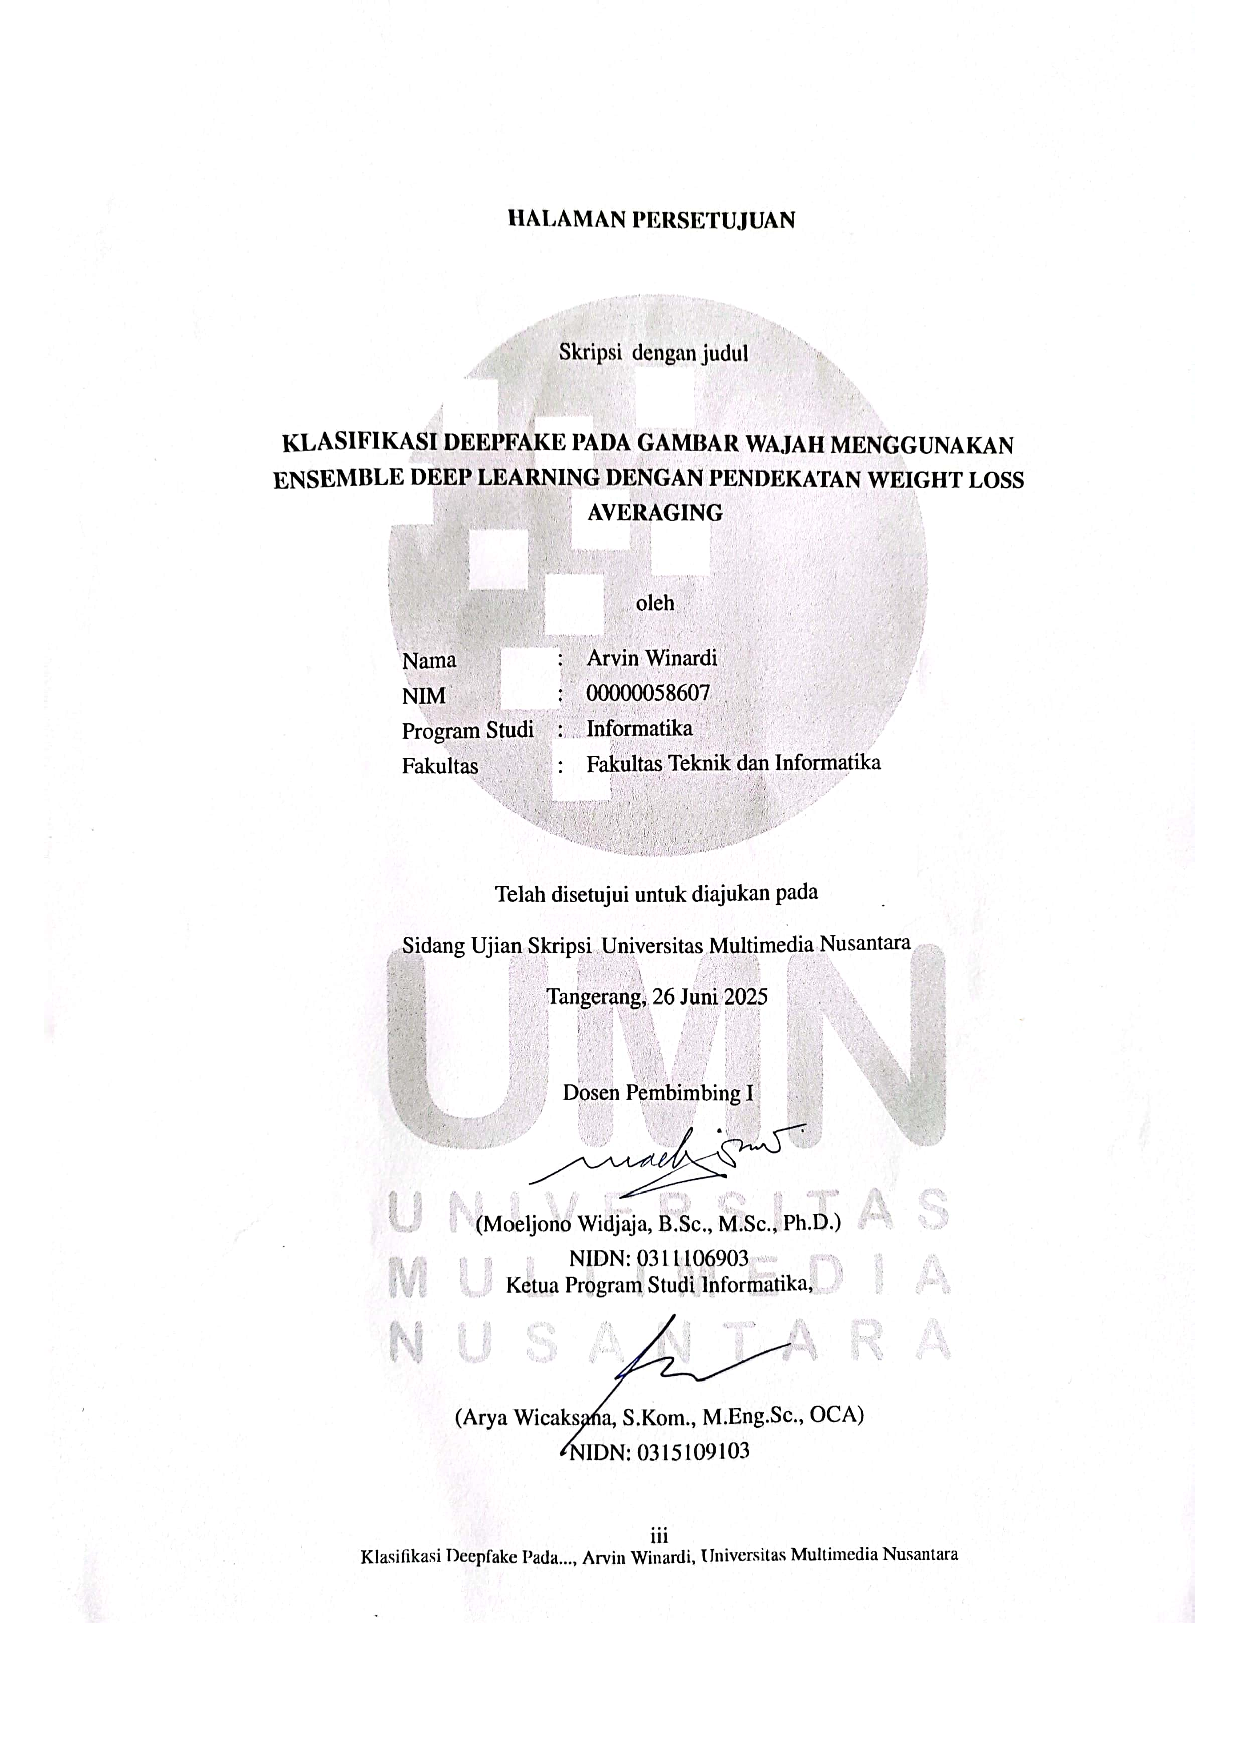
\includepdf[pages=1]{assets/pdf/halaman_persetujuan.pdf}

%
% load halaman pengesahan (jika sesudah selesai sidang) menggantikan halaman persetujuan
\addChapter{HALAMAN PENGESAHAN}
\chapter*{HALAMAN PENGESAHAN}
\onehalfspacing
\begin{center}
   \type \, dengan judul \\[0.3cm]
    
    \bo{\Judul}  \\[0.6cm]
    oleh \\[0.3cm]
\noindent
\begin{tabular}{l l p{6cm}}
	Nama&: & \penulis \\
	NIM&: & \nim \\
	Program Studi&: & Informatika \\
	Fakultas &: & Fakultas Teknik dan Informatika \\
\end{tabular} \\
\vspace{0.5em}
Telah diujikan pada hari \hariTanggalSidang \\
Pukul \waktuSidang \ dan dinyatakan \\
LULUS \\
Dengan susunan penguji sebagai berikut \\
\end{center}
\vspace*{0.3cm}
\noindent
\begin{minipage}{.5\textwidth}
\begin{center}
  Ketua Sidang \\[1.2cm]
(\ketuaSidang) \\
\ketuaSidangNIDN
\end{center}
\end{minipage}% This must go next to `\end{minipage}`
\begin{minipage}{.5\textwidth}
\begin{center}
  Penguji \\[1.2cm]
  
  (\penguji) \\
  \pengujiNIDN
    
\end{center}
\end{minipage}
\vspace*{0.1cm}
\begin{center}
     
    % Pembimbing Tunggal
    Pembimbing \\[1.2cm]
    
    
    (\pembimbing) \\
    \pembimbingNIDN
    
    
%     % Pembimbing I dan II
% \begin{minipage}{.5\textwidth}
%     \begin{center}
%         Pembimbing I\\[1.2cm]
    
    
%     (\pembimbing)
        
%     \end{center}
% \end{minipage}% This must go next to `\end{minipage}`
% \begin{minipage}{.5\textwidth}
%     \begin{center}
%             Pembimbing II\\[1.2cm]
    
    
%     (\pembimbingb) \\[0.3cm]
        
%     \end{center}
% \end{minipage}
\vspace{0.5em}
    Ketua Program Studi \program, \\[1.2cm]
    
    
    (\kaprodi) \\
    \kaprodiNIDN
    
    
\end{center}



\addChapter{HALAMAN PERSETUJUAN PUBLIKASI ILMIAH}
\chapter*{HALAMAN PERSETUJUAN PUBLIKASI KARYA ILMIAH UNTUK KEPENTINGAN AKADEMIS}

\onehalfspacing

% \vspace*{0.2cm}
\noindent 
Yang bertanda tangan di bawah ini:
% \vspace*{0.4cm}

\begin{tabular}{p{3.7cm} l p{6.5cm}}
	Nama & : & \penulis \\ 	
	NIM & : & \nim \\
	Program Studi & : & \program\\	
	Jenjang & : & \jenjang\\
	% Jenis Karya & : & \type \\
	Judul Karya Ilmiah & : & \judul \\
\end{tabular}

% \vspace*{0.6cm}
\noindent Menyatakan dengan sesungguhnya bahwa saya bersedia (\textbf{pilih salah satu}):
\begin{itemize}
    \renewcommand{\labelitemi}{${\rlap{\hspace{0.1em}$\checkmark$}}\square$}
    % \renewcommand{\labelitemi}{$\square$}
    \item Saya bersedia memberikan izin sepenuhnya kepada Universitas Multimedia Nusantara untuk mempublikasikan hasil karya ilmiah saya ke dalam repositori Knowledge Center sehingga dapat diakses oleh Sivitas Akademika UMN/Publik. Saya menyatakan bahwa karya ilmiah yang saya buat tidak mengandung data yang bersifat konfidensial. 

    % \renewcommand{\labelitemi}{${\rlap{\hspace{0.1em}$\checkmark$}}\square$}
    \renewcommand{\labelitemi}{$\square$}
    \item Saya tidak bersedia mempublikasikan hasil karya ilmiah ini ke dalam repositori Knowledge Center, dikarenakan: dalam proses pengajuan publikasi ke jurnal/konferensi nasional/internasional (dibuktikan dengan \textit{letter of acceptance}) **.
    \item Lainnya, pilih salah satu:
    \begin{itemize} 
    \renewcommand{\labelitemi}{$\square$}
        \item Hanya dapat diakses secara internal Universitas Multimedia Nusantara
        \item Embargo publikasi karya ilmiah dalam kurun waktu tiga tahun.
    \end{itemize}
\end{itemize}

\begin{flushright}
Tangerang, \tanggalPengumpulan \\
Yang menyatakan\\[2.5cm]
\noindent
\penulis
\end{flushright}


\vfill

% \singlespacing
% {
% \footnotesize
% \noindent **Jika tidak bisa membuktikan LoA jurnal/HKI, saya bersedia mengizinkan penuh karya ilmiah saya untuk dipublikasikan ke KC UMN dan menjadi hak institusi UMN.
% }

\onehalfspacing
\newpage
\clearpage


% \addChapter{HALAMAN PERSEMBAHAN/MOTO}
% \chapter*{\uppercase{Halaman Persembahan / Motto}}

\vspace{2cm}
\begin{quote}
    
"A good name is to be more desired than great wealth,
Favor is better than silver and gold."

\end{quote}

\hfill Proverbs 22:1 (NASB)
% \clearpage


\addChapter{KATA PENGANTAR}
\chapter*{KATA PENGANTAR}
% \onehalfspacing
Puji syukur atas berkat dan rahmat kepada Tuhan Yang Maha Esa, atas selesainya pembuatan Tugas Akhir dengan judul “KLASIFIKASI DEEPFAKE PADA GAMBAR WAJAH MENGGUNAKAN
ENSEMBLE DEEP LEARNING DENGAN PENDEKATAN WEIGHT LOSS
AVERAGING”. Tugas akhir ini dibuat sebagai syarat untuk mencapai gelar Sarjana Komputer
Jurusan Informatika pada Fakultas Teknik dan Informatika Universitas Multimedia Nusantara. Saya menyadari bahwa, tanpa bantuan dan bimbingan dari berbagai pihak, dari masa perkuliahan sampai pada penyusunan laporan magang ini, sangatlah sulit bagi saya untuk menyelesaikan laporan skripsi ini. Oleh karena itu, saya mengucapkan terima kasih kepada :

\noindent Mengucapkan terima kasih
\begin{enumerate}
	\item Bapak \rektorUMN, selaku Rektor Universitas Multimedia
Nusantara. 
	\item Bapak \dekanFTI, selaku Dekan Fakultas Teknik dan
Informatika Universitas Multimedia Nusantara.
	\item Bapak \kaprodi, selaku Ketua Program Studi
Informatika Universitas Multimedia Nusantara. 
	\item Bapak \pembimbing,  sebagai Pembimbing pertama yang telah memberikan bimbingan, arahan, dan motivasi atas terselesainya tugas akhir ini.
% \item Bapak/Ibu \pembimbingb, sebagai Pembimbing kedua (*jika ada dua Pembimbing) yang telah memberikan bimbingan, arahan, dan motivasi atas terselesainya tugas akhir ini. 
\item Orang Tua dan keluarga saya yang telah memberikan bantuan dukungan material dan moral, sehingga penulis dapat menyelesaikan tesis ini.
\item Keluarga saya yang telah memberikan bantuan dukungan material dan moral, sehingga penulis dapat menyelesaikan tugas akhir ini. 
\end{enumerate}
% (harapan) Semoga karya ilmiah ini

\vspace*{0.1cm}

\begin{flushright}
Tangerang, \tanggalPengumpulan \\[0.1cm]
\vspace*{2cm}
\penulis
\end{flushright}
\clearpage


\addChapter{ABSTRAK}
%-----------------------------------------------------------------------------%
\chapter*{\Judul}
%-----------------------------------------------------------------------------%
\singlespacing
\begin{center}
    
    \vspace{-4em}
    
    \penulis
    
	\bigskip
    
    \textbf{ABSTRAK}
    
\end{center}

% \chapter*{Abstrak}

\vspace*{0.2cm}
{
	\setlength{\parindent}{0pt}

	\bigskip
	\bigskip

    \noindent
    Kemajuan teknologi \textit{deepfake} telah menimbulkan tantangan signifikan dalam menjaga integritas informasi digital. Penelitian ini mengusulkan sistem klasifikasi \textit{deepfake} pada gambar wajah menggunakan pendekatan \textit{ensemble deep learning} dengan metode \textit{weighted averaging}. Empat model individu digunakan dalam ansambel: Custom CNN, ResNet50, Xception, dan EfficientNet-B4. Dataset yang digunakan adalah \textit{140k Real and Fake Faces} dari Kaggle, dengan partisi data pelatihan, validasi, dan pengujian sebesar 100.000, 20.000, dan 20.000 gambar. Setiap model dilatih secara independen dan dievaluasi menggunakan metrik Akurasi, Presisi, Recall, F1-Score. Hasil eksperimen menunjukkan bahwa model ansambel menghasilkan akurasi sebesar 96.87\%, lebih tinggi dibandingkan model individual terbaik (Xception, 95.83\%). Evaluasi \textit{cross-dataset} menggunakan \textit{DeepFakeFace} menunjukkan bahwa meskipun akurasi menurun menjadi 50\%, ansambel tetap menunjukkan kinerja generalisasi yang lebih baik dibandingkan model tunggal. Penelitian ini menunjukkan bahwa pendekatan \textit{ensemble} dengan arsitektur yang beragam dapat meningkatkan akurasi dan keandalan sistem deteksi \textit{deepfake}.
	\bigskip
% Kata kunci urut abjad

	\textbf{Kata kunci}: 	\textit{Deepfake, Image Detection, Ensemble Learning, Weighted Averaging, CNN}
}

\onehalfspacing
\clearpage

\addChapter{ABSTRACT}
%-----------------------------------------------------------------------------%
\chapter*{\MakeUppercase{ \JudulInggris}}
%-----------------------------------------------------------------------------%
\singlespacing
\begin{center}
    
    \vspace{-4em}
    
    \penulis
    
	\bigskip
    
    \textbf{ABSTRACT}
    
\end{center}

% \chapter*{Abstrak}

\vspace*{0.2cm}
{
	\setlength{\parindent}{0pt}

	\bigskip
	\bigskip

        \noindent
        \textit{The advancement of \textit{deepfake} technology poses significant challenges in preserving the integrity of digital information. This study proposes a facial image \textit{deepfake} classification system using an \textit{ensemble deep learning} approach with \textit{weighted averaging}. Four individual models were employed in the ensemble: Custom CNN, ResNet50, Xception, and EfficientNet-B4. The dataset used was the \textit{140k Real and Fake Faces} from Kaggle, partitioned into 100,000 training, 20,000 validation, and 20,000 test images. Each model was trained independently and evaluated using Accuracy, Precision, Recall, F1-Score. Experimental results show that the ensemble model achieved an accuracy of 96.87\%, outperforming the best individual model (Xception, 95.83\%). Cross-dataset evaluation on \textit{DeepFakeFace} demonstrated that although the accuracy dropped to 50\%, the ensemble still exhibited superior generalization performance compared to single models. This research highlights that ensemble methods with diverse architectures can enhance the accuracy and reliability of deepfake detection systems.}

	\bigskip
% keywords in alphabetical order

	\textit{\textbf{Keywords}}: 	\textit{Deepfake, Image Detection, Ensemble Learning, Weighted Averaging, CNN}
}

\onehalfspacing
\clearpage


%
% Daftar isi, gambar, tabel, dan kode
%
\singlespacing

\phantomsection
%  \pagestyle{daftarIsi}
\pagestyle{plain}
\tableofcontents
\clearpage

\phantomsection
\listoftables
\clearpage

\phantomsection
\listoffigures
\clearpage

% \phantomsection
% \lstlistoflistings
% \clearpage



\phantomsection
\listofequation
\addChapter{DAFTAR RUMUS}
\clearpage

\phantomsection
\listofappendices
\addChapter{DAFTAR LAMPIRAN}
\clearpage


\onehalfspacing

\pagestyle{fancy}

%
% Gunakan penomeran Arab (1, 2, 3, ...) setelah bagian ini.
%
\pagenumbering{arabic}

%
% Isi Skripsi
%

\BgThispage

%-----------------------------------------------------------------------------%
\chapter{PENDAHULUAN}
%-----------------------------------------------------------------------------%

%-----------------------------------------------------------------------------%
\section{Latar Belakang Masalah}
%-----------------------------------------------------------------------------%

Perkembangan pesat teknologi kecerdasan buatan telah melahirkan berbagai inovasi dalam bidang pengolahan citra digital, salah satunya adalah teknologi \textit{deepfake}. Istilah \textit{deepfake}, yang merupakan lakuran dari frasa "\textit{deep learning}" dan "\textit{fake}", merujuk pada teknik manipulasi media yang menggunakan algoritma pembelajaran mendalam untuk menghasilkan konten audio dan visual sintetis yang tampak otentik \cite{rana2022deepfake}. Teknologi ini umumnya memanfaatkan arsitektur \textit{Generative Adversarial Networks} (GANs) untuk menciptakan representasi wajah yang sangat realistis dengan menggantikan identitas seseorang dalam sebuah video atau gambar \cite{goodfellow2014gan}.

Kemunculan teknologi \textit{deepfake} pertama kali dipopulerkan oleh pengguna forum daring Reddit pada akhir tahun 2017. Pengguna tersebut mengaplikasikan metode \textit{deep learning} untuk memanipulasi wajah dalam konten video \cite{edwards2024}. Sejak saat itu, aksesibilitas terhadap teknologi ini terus meningkat seiring dengan berkembangnya berbagai aplikasi tingkat konsumen seperti FaceApp dan FaceSwap, yang memungkinkan pengguna awam untuk membuat konten \textit{deepfake} dengan mudah.

Meskipun teknologi \textit{deepfake} memiliki potensi aplikasi positif dalam industri hiburan, pendidikan, dan simulasi medis, dampak negatifnya terhadap masyarakat telah menjadi sorotan utama. Penggunaan teknologi ini dengan niat jahat dapat menghasilkan konten yang menyesatkan, menyebarkan misinformasi, dan mengancam integritas digital \cite{dagar2022deepfake}. Salah satu kasus viral yang menunjukkan potensi destabilisasi sosial dan politik adalah video \textit{deepfake} Presiden Ukraina, Volodymyr Zelenskyy, yang seolah-olah menyerah kepada Rusia pada tahun 2022 \cite{tyagi2023analysis}.

Mengingat ancaman serius yang ditimbulkan oleh \textit{deepfake}, pengembangan sistem deteksi yang akurat dan andal menjadi sebuah kebutuhan yang mendesak. Pendekatan deteksi \textit{deepfake} secara umum dapat dikategorikan menjadi tiga jenis: \textit{naive detectors} yang menggunakan arsitektur CNN sederhana, \textit{spatial detectors} yang mengeksplorasi artefak spasial, dan \textit{frequency detectors} yang menganalisis domain frekuensi \cite{verdoliva2020deepfake}. Namun, peningkatan kualitas \textit{deepfake} yang dihasilkan oleh teknik-teknik generasi terbaru menuntut pengembangan metode deteksi yang lebih canggih.

Arsitektur \textit{deep learning} telah menunjukkan keunggulan signifikan dalam tugas deteksi \textit{deepfake} jika dibandingkan dengan metode konvensional yang berbasis pada fitur rekayasa tangan. Keunggulan ini terletak pada kemampuan model untuk mempelajari representasi fitur secara otomatis langsung dari data, sehingga memungkinkan adaptasi yang lebih baik terhadap berbagai teknik manipulasi \cite{lecun2015deep}. Berbagai arsitektur CNN termutakhir seperti ResNet \cite{he2016deep}, Xception \cite{szegedy2016rethinking}, dan EfficientNet \cite{tan2019efficientnet} telah diaplikasikan untuk deteksi \textit{deepfake} dengan hasil yang menjanjikan.

\subsection{Tantangan dan Keterbatasan Model Tunggal}

Meskipun model tunggal menunjukkan performa yang baik, penelitian menunjukkan bahwa model tersebut sering kali memiliki keterbatasan dalam melakukan generalisasi terhadap teknik-teknik manipulasi baru yang terus berkembang. Variasi dalam metode pembuatan \textit{deepfake}, kualitas set data, dan kondisi dunia nyata menuntut model deteksi untuk memiliki kemampuan generalisasi yang tinggi \cite{edwards2024}. 

Penelitian terbaru menunjukkan bahwa berbagai metode deteksi \textit{deepfake} memiliki performa yang bervariasi pada dataset yang berbeda. Metode POI-DeepFake yang menggunakan ResNet50 menunjukkan konsistensi performa yang baik di berbagai dataset dengan akurasi berkisar 81,10\%-86,80\% \cite{cozzolino2023}. Sementara itu, pendekatan \textit{hybrid} seperti DCPT yang menggabungkan CNN dengan \textit{Vision Transformer} menunjukkan performa sangat baik pada dataset tertentu (92,11\% pada FF++) namun kurang konsisten pada dataset lainnya (63,27\% pada CelebDF) \cite{wang2023deep}.

Penggunaan arsitektur \textit{Xception} dalam beberapa penelitian seperti Si-Net, ISTVT, dan FAAF menunjukkan performa yang konsisten dan kompetitif, dengan akurasi berkisar 94,54\%-99,85\% tergantung pada dataset evaluasi \cite{wang2023si,zhao2023,tian2023}. Model \textit{EfficientNet} juga menunjukkan keunggulan dalam hal efisiensi komputasi dengan performa yang kompetitif \cite{ke2023}. Namun, variabilitas performa ini mengindikasikan bahwa tidak ada satu arsitektur yang dominan untuk semua skenario, dan setiap model memiliki kelebihan dan kekurangan yang berbeda.

\subsection{Potensi Ensemble Learning}

Oleh karena itu, pendekatan \textit{ensemble learning} yang menggabungkan beberapa model dengan karakteristik yang saling melengkapi menjadi strategi yang menjanjikan untuk meningkatkan akurasi dan keandalan sistem deteksi. \textit{Ensemble learning} adalah sebuah teknik yang menggabungkan prediksi dari beberapa model dasar untuk menghasilkan keputusan akhir yang lebih akurat dan stabil dibandingkan model individual \cite{dietterich2000ensemble}. Dalam konteks deteksi \textit{deepfake}, metode ansambel dapat menutupi kelemahan model-model individual dan meningkatkan kemampuan deteksi terhadap berbagai jenis manipulasi.

Penelitian terbaru menunjukkan bahwa ansambel dengan metode \textit{weighted averaging} memberikan kinerja yang unggul dalam deteksi \textit{deepfake} dibandingkan teknik ansambel konvensional. Metode ini menghitung kontribusi setiap model dasar berdasarkan kinerjanya pada set data validasi, sehingga model dengan akurasi lebih tinggi akan mendapatkan bobot yang lebih besar dalam pengambilan keputusan akhir. Pendekatan ini tidak hanya meningkatkan akurasi, tetapi juga memberikan interpretabilitas yang lebih baik mengenai kontribusi setiap model.

\subsection{Pemilihan Arsitektur untuk Model Ensemble}

Berdasarkan analisis literatur, kombinasi model-model dengan karakteristik arsitektur yang beragam dapat memberikan komplementaritas yang optimal untuk sebuah ansambel. Pemilihan arsitektur-arsitektur dalam penelitian ini didasarkan pada rekam jejak dan karakteristiknya yang saling melengkapi:

\textit{Custom CNN} dirancang khusus untuk tugas deteksi dengan arsitektur hierarkis yang memanfaatkan karakteristik CNN dalam ekstraksi fitur lokal-ke-global. Model ini dapat mendeteksi inkonsistensi yang umum pada citra \textit{deepfake} melalui pembelajaran fitur dari level rendah hingga level tinggi.

\textit{ResNet50} dengan mekanisme \textit{residual learning} telah terbukti andal dalam berbagai literatur ilmiah dan kompetisi pengolahan citra \cite{he2016deep}. Arsitektur ini menggunakan \textit{shortcut connections} yang memungkinkan pelatihan jaringan yang sangat dalam tanpa mengalami masalah \textit{vanishing gradient}.

\textit{Xception} dengan \textit{depthwise separable convolutions} menawarkan pendekatan ekstraksi fitur yang efisien dengan memisahkan operasi konvolusi spatial dan \textit{channel-wise} \cite{chollet2017xception}. Pendekatan ini mengurangi kompleksitas komputasi sambil mempertahankan kemampuan representasi fitur yang kuat.

\textit{EfficientNet} dengan \textit{compound scaling} menyeimbangkan kedalaman, lebar, dan resolusi input secara simultan, menghasilkan model yang efisien tanpa mengorbankan akurasi \cite{tan2019efficientnet}. Strategi ini mengoptimalkan performa sistem secara menyeluruh.

Keragaman pendekatan ekstraksi fitur yang mereka tawarkan menjadi kunci utama dalam metode ansambel, di mana model-model dengan pola kesalahan yang berbeda cenderung dapat saling mengoreksi, sehingga berpotensi meningkatkan akurasi dan keandalan sistem deteksi secara keseluruhan.

Pemilihan set data yang tepat juga merupakan faktor krusial dalam pengembangan sistem deteksi \textit{deepfake}. Set data "140k Real and Fake Faces" dipilih dalam penelitian ini karena menyediakan keseimbangan yang baik antara data asli dan sintetis, dengan standardisasi format yang konsisten serta keragaman yang memadai untuk proses pelatihan dan evaluasi yang andal.

Oleh karena itu, penelitian ini bertujuan untuk mengembangkan dan mengevaluasi sistem deteksi \textit{deepfake} menggunakan metode \textit{ensemble weighted averaging} yang menggabungkan empat arsitektur \textit{deep learning} yang berbeda: Custom CNN, ResNet50, Xception, dan EfficientNet. Pendekatan ini diharapkan dapat memberikan kontribusi signifikan dalam peningkatan akurasi dan keandalan deteksi \textit{deepfake}, serta memberikan wawasan mengenai efektivitas metode ansambel dalam domain \textit{computer vision security}.

%-----------------------------------------------------------------------------%
\section{Rumusan Masalah}
%-----------------------------------------------------------------------------%

Berdasarkan latar belakang yang telah diuraikan, rumusan masalah dalam penelitian ini adalah sebagai berikut:

\begin{enumerate}
\item Bagaimanakah perbandingan kinerja metode \textit{ensemble learning} dengan teknik \textit{weighted averaging} dibandingkan dengan kinerja model-model individual dalam mengklasifikasikan citra \textit{deepfake}?

\item Apakah metode ansambel menunjukkan kemampuan generalisasi pada skenario pengujian \textit{cross-dataset} yang secara signifikan lebih unggul dibandingkan dengan kemampuan generalisasi masing-masing model tunggal penyusunnya?
\end{enumerate}

%-----------------------------------------------------------------------------%
\section{Batasan Masalah}
%-----------------------------------------------------------------------------%

Untuk menjaga agar penelitian ini tetap fokus dan terarah, ditetapkan beberapa batasan masalah sebagai berikut:

\subsection{Batasan Set Data dan Pra-pemrosesan}
\begin{enumerate}
\item Penelitian ini hanya menggunakan set data "140k Real and Fake Faces" yang terdiri dari 140.000 citra wajah berformat JPEG dengan resolusi 256×256 piksel.

\item Set data dibagi menjadi tiga bagian dengan rasio 100.000 untuk pelatihan, 20000 untuk validasi, dan 20000 untuk pengujian.

\item Proses \textit{preprocessing} data terbatas pada normalisasi nilai piksel (penyekalaan ulang ke rentang 0–1) dan augmentasi data berupa pembalikan horizontal pada data pelatihan.

\item Penelitian ini berfokus pada deteksi \textit{deepfake} berbasis citra statis dan tidak mencakup analisis pada sekuens video.
\end{enumerate}

\subsection{Batasan Arsitektur Model}
\begin{enumerate}
\item Model ansambel terdiri dari empat arsitektur: Custom CNN, ResNet50, Xception, dan EfficientNet-B4.

\item Model ResNet50, Xception, dan EfficientNet memanfaatkan mekanisme \textit{transfer learning} dengan menggunakan bobot pra-terlatih dari set data ImageNet.

\item Arsitektur Custom CNN dirancang dengan 4 blok konvolusional yang diikuti oleh lapisan terhubung penuh.

\item Metode ansambel yang digunakan terbatas pada \textit{weighted averaging} yang bobotnya ditentukan berdasarkan akurasi validasi.
\end{enumerate}

\subsection{Batasan Evaluasi}
\begin{enumerate}
\item Metrik yang digunakan untuk evaluasi kinerja meliputi Akurasi, Presisi, Perolehan (\textit{Recall}), dan Skor-F1

\item Evaluasi kinerja model dilakukan melalui dua skenario pengujian utama:
\begin{itemize}
    \item \textbf{Pengujian internal:} Menggunakan test set yang berasal dari partisi dataset utama "140k Real and Fake Faces" untuk mengukur performa model pada data dengan distribusi serupa.
    \item \textbf{Pengujian Generalisasi (Cross-Dataset):} Menggunakan dataset eksternal "DeepFakeFace" untuk menguji kemampuan generalisasi dan robustisitas model terhadap data deepfake yang dibuat dengan teknik berbeda dan tidak pernah dilihat sebelumnya.
\end{itemize}
\end{enumerate}

\subsection{Batasan Teknis}
\begin{enumerate}
\item Proses pelatihan model dilakukan menggunakan platform Google Colab Pro+ dengan GPU Nvidia T4 dan RAM 16 GB.

\item Implementasi model menggunakan kerangka kerja TensorFlow/Keras dengan bahasa pemrograman Python 3.8+.

\item Jumlah maksimum epoch pelatihan adalah 15, dengan mekanisme penghentian dini pada patience 3.
\end{enumerate}

%-----------------------------------------------------------------------------%
\section{Tujuan Penelitian}
%-----------------------------------------------------------------------------%

Berdasarkan rumusan masalah yang telah ditetapkan, penelitian ini memiliki tujuan umum dan khusus sebagai berikut:

\begin{enumerate}
\item \textbf{Tujuan Umum:} \\
Mengembangkan dan mengevaluasi sebuah sistem deteksi \textit{deepfake} berbasis \textit{ensemble learning} untuk menghasilkan metode klasifikasi yang tidak hanya akurat tetapi juga memiliki kemampuan generalisasi yang andal.

\item \textbf{Tujuan Khusus:} \\
Secara spesifik, penelitian ini bertujuan untuk:
\begin{enumerate}
    \item Membandingkan kinerja metode \textit{ensemble learning} dengan teknik \textit{weighted averaging} terhadap kinerja masing-masing model individual (Custom CNN, ResNet50, Xception, dan EfficientNet) dalam mengklasifikasikan citra \textit{deepfake}.
    
    \item Menguji apakah pendekatan ansambel menunjukkan kemampuan generalisasi yang secara signifikan lebih unggul dibandingkan dengan setiap model individual ketika dihadapkan pada skenario pengujian \textit{cross-dataset}.
\end{enumerate}

\item \textbf{Indikator Evaluasi dan Metode Pengukuran} \\
Pencapaian tujuan penelitian ini akan dievaluasi menggunakan indikator-indikator berikut:

\begin{enumerate}
    \item \textbf{Peningkatan Akurasi}: Diukur melalui perbandingan nilai akurasi ensemble dengan model individual terbaik.
    
    \item \textbf{Konsistensi Metrik}: Evaluasi menggunakan empat metrik utama (Accuracy, Precision, Recall, F1-Score) pada dataset pengujian.
    
    \item \textbf{Kemampuan Generalisasi}: Diukur melalui pengujian cross-dataset menggunakan dataset eksternal (DeepFakeFace) dengan membandingkan penurunan performa ensemble vs model individual.
    
    \item \textbf{Komplementaritas Model}: Dianalisis melalui confusion matrix dan distribusi bobot ensemble untuk memvalidasi kontribusi setiap model.
\end{enumerate}
\end{enumerate}

%-----------------------------------------------------------------------------%
\section{Manfaat Penelitian}
%-----------------------------------------------------------------------------%

Penelitian ini diharapkan dapat memberikan manfaat pada berbagai aspek sebagai berikut:

\subsection{Manfaat Teoritis}
\begin{enumerate}
    \item \textbf{Pengembangan Metode Ensemble}: Memberikan kontribusi pada pengembangan teknik \textit{weighted averaging} untuk meningkatkan akurasi sistem deteksi \textit{deepfake} secara signifikan.
    
    \item \textbf{Validasi Komplementaritas Model}: Membuktikan secara empiris bahwa kombinasi arsitektur CNN yang beragam dapat meningkatkan robustisitas deteksi dengan mengurangi \textit{false negative} dan \textit{false positive}.
    
    \item \textbf{Framework Evaluasi}: Menyediakan kerangka evaluasi komprehensif untuk sistem deteksi \textit{deepfake} yang mencakup pengujian \textit{cross-dataset} untuk mengukur kemampuan generalisasi.
\end{enumerate}

\subsection{Manfaat Praktis}
\begin{enumerate}
    \item \textbf{Peningkatan Akurasi Deteksi}: Sistem ensemble yang dihasilkan mencapai akurasi 99,64\%, meningkatkan kemampuan deteksi \textit{deepfake} untuk implementasi pada platform media sosial dan sistem verifikasi berita.
    
    \item \textbf{Optimalisasi Computational Trade-off}: Memberikan keseimbangan antara akurasi tinggi dan efisiensi komputasi melalui kombinasi model yang ter-optimasi.
    
    \item \textbf{Aplikabilitas Industri}: Menyediakan solusi praktis yang dapat diintegrasikan dalam sistem moderasi konten \textit{real-time} dan analisis forensik digital.
\end{enumerate}

\subsection{Manfaat Akademis}
\begin{enumerate}
    \item \textbf{Referensi dan Tolok Ukur (\textit{Benchmark})}: Menjadi referensi dan menyediakan tolok ukur kinerja (\textit{benchmark}) untuk implementasi metode \textit{ensemble weighted averaging} pada tugas deteksi \textit{deepfake}, yang dapat dimanfaatkan oleh komunitas akademik untuk penelitian selanjutnya.
    
    \item \textbf{Dasar Pengembangan Lanjutan}: Menyediakan dasar dan wawasan untuk pengembangan metode deteksi \textit{deepfake} yang lebih maju, khususnya dalam eksplorasi arsitektur yang komplementer dan teknik ansambel yang lebih canggih.
\end{enumerate}

\subsection{Manfaat Sosial}
\begin{enumerate}
    \item \textbf{Literasi Media}: Berkontribusi pada upaya peningkatan kemampuan masyarakat untuk mengidentifikasi konten manipulatif di era digital.
    
    \item \textbf{Integritas Informasi}: Mendukung terjaganya kebenaran dan kepercayaan dalam ekosistem informasi digital melalui teknologi deteksi yang canggih.
    
    \item \textbf{Pengembangan AI yang Etis}: Memberikan contoh penggunaan kecerdasan buatan untuk tujuan defensif dan protektif, menyeimbangkan kemajuan teknologi generatif dengan kapabilitas untuk memitigasi risikonya.
\end{enumerate}

%-----------------------------------------------------------------------------%
\section{Sistematika Penulisan}
%-----------------------------------------------------------------------------%

Laporan penelitian ini disusun secara sistematis dan logis untuk memberikan pemahaman yang komprehensif mengenai penelitian yang dilakukan. Struktur penulisan terdiri dari lima bab utama dengan rincian sebagai berikut:

\begin{itemize}
\item \textbf{Bab I - PENDAHULUAN}
Bab ini menguraikan latar belakang yang menjelaskan urgensi pengembangan sistem deteksi \textit{deepfake}, rumusan masalah, batasan-batasan penelitian, tujuan yang ingin dicapai, manfaat teoretis dan praktis, serta sistematika penulisan laporan.

\item \textbf{Bab II - TINJAUAN PUSTAKA}
Bab ini menyajikan tinjauan pustaka dan landasan teori yang relevan, mencakup konsep fundamental kecerdasan buatan dan \textit{deep learning}, teknologi \textit{deepfake} dan \textit{Generative Adversarial Networks}, arsitektur \textit{deep learning} yang digunakan (CNN, ResNet, Xception, EfficientNet), teori \textit{ensemble learning} dan \textit{weighted averaging}, serta metrik evaluasi yang komprehensif.

\item \textbf{Bab III - METODOLOGI PENELITIAN}
Bab ini menjelaskan metodologi penelitian secara terperinci, meliputi desain penelitian dan alur kerja eksperimen, karakteristik dan proses pra-pemrosesan set data, arsitektur dan konfigurasi setiap model individual, implementasi metode \textit{ensemble weighted averaging}, prosedur pelatihan dan penalaan hiperparameter, serta lingkungan komputasi dan reprodusibilitas.

\item \textbf{Bab IV - HASIL DAN PEMBAHASAN}
Bab ini menyajikan hasil eksperimen beserta pembahasan yang komprehensif. Cakupannya meliputi analisis kinerja setiap model \textit{deep learning} secara individual, hasil implementasi sistem ansambel, perbandingan kuantitatif antara pendekatan individual dan ansambel, analisis kontribusi dan komplementaritas antar model, interpretasi hasil dalam konteks metode termutakhir, serta pembahasan mengenai limitasi dan implikasi dari temuan penelitian.

\item \textbf{Bab V - KESIMPULAN DAN SARAN}
Bab ini berisi kesimpulan penelitian yang menjawab rumusan masalah berdasarkan hasil eksperimen, menguraikan kontribusi ilmiah yang dihasilkan, mengidentifikasi keterbatasan penelitian, serta memberikan saran untuk pengembangan penelitian selanjutnya dan implementasi praktis dalam aplikasi dunia nyata.
\end{itemize}
%-----------------------------------------------------------------------------%
\chapter{\babDua}

Bab ini menyajikan tinjauan pustaka yang melandasi penelitian deteksi \textit{deepfake} menggunakan \textit{ensemble weighted averaging}. Pembahasan mencakup fondasi \textit{deep learning}, arsitektur CNN modern, metodologi \textit{ensemble learning}, teknologi \textit{deepfake}, dan aspek evaluasi. Setiap bagian dirancang untuk membangun pemahaman progresif menuju implementasi sistem deteksi yang robust dan akurat.

%-----------------------------------------------------------------------------%
\section{Fondasi Deep Learning untuk Computer Vision}
%-----------------------------------------------------------------------------%

Pemahaman mendalam tentang fondasi \textit{deep learning} menjadi prasyarat untuk mengembangkan sistem deteksi \textit{deepfake} yang efektif. Bagian ini membangun fondasi teoritis dengan fokus pada konsep yang secara langsung relevan untuk deteksi manipulasi visual, menghindari pembahasan yang terlalu umum namun memastikan pemahaman yang solid.

\subsection{Machine Learning dan Deep Learning}

\textit{Machine learning} merupakan paradigma revolusioner dalam kecerdasan buatan yang memungkinkan sistem belajar dari data tanpa pemrograman eksplisit untuk setiap tugas spesifik \cite{mitchell1997machine}. Paradigma ini mengubah pendekatan tradisional pemrograman dimana aturan-aturan eksplisit dikodekan secara manual, menjadi pendekatan dimana sistem secara otomatis mengidentifikasi pola dari data untuk membuat prediksi atau keputusan.

Dalam konteks deteksi \textit{deepfake}, pemahaman tentang kategorisasi \textit{machine learning} menjadi krusial. \textit{Supervised learning} menjadi pendekatan utama dalam penelitian ini, dimana model belajar dari dataset berlabel yang terdiri dari citra asli dan citra manipulasi. Proses pembelajaran ini memungkinkan model untuk mengidentifikasi perbedaan halus antara konten autentik dan sintetis. \textit{Unsupervised learning} dapat digunakan untuk menemukan pola tersembunyi dalam data tanpa label, sementara \textit{reinforcement learning} berpotensi untuk pembelajaran adaptif terhadap evolusi teknik \textit{deepfake}.

\textit{Deep Learning} merepresentasikan evolusi signifikan dari \textit{machine learning} tradisional melalui penggunaan jaringan saraf berlapis (\textit{deep neural networks}) untuk mengekstrak representasi fitur secara hierarkis \cite{lecun2015deep}. Revolusi ini terjadi karena kemampuan \textit{deep learning} dalam menangani kompleksitas data visual yang tinggi, seperti citra dan video, yang merupakan domain utama teknologi \textit{deepfake}.

Keunggulan fundamental \textit{deep learning} terletak pada kemampuan \textit{automatic feature extraction}. Berbeda dengan pendekatan tradisional yang memerlukan \textit{hand-crafted features} - dimana pakar domain harus secara manual merancang fitur-fitur yang relevan seperti \textit{edge detectors}, \textit{texture descriptors}, atau \textit{statistical measures} - \textit{deep learning} dapat secara otomatis mempelajari representasi optimal langsung dari data mentah \cite{bengio2013representation}. Dalam konteks deteksi \textit{deepfake}, kemampuan ini sangat krusial karena artefak manipulasi seringkali sangat halus dan sulit diidentifikasi secara manual.

Proses pembelajaran hierarkis dalam \textit{deep learning} memungkinkan model untuk membangun pemahaman dari fitur-fitur sederhana (seperti tepi dan tekstur) pada lapisan awal, menuju konsep yang lebih kompleks (seperti fitur wajah dan konten semantik) pada lapisan yang lebih dalam. Hierarki ini sangat sesuai dengan sifat deteksi \textit{deepfake}, dimana inkonsistensi dapat terjadi pada berbagai tingkat abstraksi.

\subsection{Neural Networks: Konsep Dasar}

\textit{Neural networks} merupakan arsitektur komputasi yang terinspirasi dari cara kerja otak manusia, terdiri dari unit-unit pemrosesan sederhana (neuron) yang saling terhubung untuk membentuk jaringan kompleks yang mampu mempelajari pola dari data. Pemahaman yang solid tentang konsep dasar ini esensial untuk mengapresiasi kompleksitas arsitektur modern yang digunakan dalam deteksi \textit{deepfake}.

Struktur dasar \textit{neural network} terdiri dari tiga komponen fundamental. Lapisan masukan berfungsi sebagai gerbang yang menerima data mentah - dalam konteks deteksi \textit{deepfake}, ini berupa nilai piksel dari citra masukan. Lapisan tersembunyi (\textit{hidden layers}) melakukan transformasi non-linear yang kompleks terhadap data, mengekstrak dan mengkombinasikan fitur-fitur pada berbagai tingkat abstraksi. Lapisan keluaran menghasilkan prediksi akhir - untuk deteksi \textit{deepfake}, ini berupa probabilitas bahwa masukan adalah konten manipulasi.

Setiap koneksi dalam jaringan memiliki bobot (\textit{weight}) yang menentukan kekuatan sinyal yang ditransmisikan antar neuron. Proses pembelajaran pada dasarnya adalah proses optimisasi bobot-bobot ini melalui paparan terhadap data pelatihan. Selain bobot, setiap neuron juga memiliki bias yang memungkinkan model untuk membuat penyesuaian yang lebih fleksibel terhadap ambang aktivasi.

Fungsi aktivasi memainkan peran krusial dalam memperkenalkan non-linearitas yang memungkinkan jaringan mempelajari pola kompleks. Tanpa non-linearitas, jaringan hanya akan mampu mempelajari transformasi linear, yang sangat terbatas dalam menangani kompleksitas data visual. Visualisasi setiap fungsi aktivasi dapat dilihat pada Gambar \ref{fig:activation_graph}.

\textbf{ReLU (Rectified Linear Unit)} telah menjadi fungsi aktivasi dominan dalam \textit{deep learning} modern karena kesederhanaannya yang elegan dan efektivitasnya yang terbukti:
\begin{equation}
\text{ReLU}(x) = \max(0, x)
\label{eq:relu}
\end{equation}

ReLU mengatasi masalah \textit{vanishing gradient} yang sering terjadi dengan fungsi aktivasi tradisional seperti sigmoid atau tanh, memungkinkan pelatihan jaringan yang sangat dalam dengan lebih efektif.

\textbf{Sigmoid} tetap penting khususnya untuk lapisan keluaran dalam klasifikasi biner seperti deteksi \textit{deepfake}:
\begin{equation}
\sigma(x) = \frac{1}{1 + e^{-x}}
\label{eq:sigmoid}
\end{equation}

Sigmoid menghasilkan keluaran dalam rentang (0,1) yang dapat diinterpretasikan sebagai probabilitas, sangat sesuai untuk tugas klasifikasi biner. 

Proses pelatihan jaringan saraf melibatkan dua fase fundamental. \textit{Forward propagation} mengalirkan data dari masukan menuju keluaran, menghasilkan prediksi berdasarkan bobot saat ini. Untuk setiap lapisan, proses ini dapat diformulasikan sebagai:

\begin{align}
z^{(l)} &= W^{(l)} a^{(l-1)} + b^{(l)} \label{eq:forward_z} \\
a^{(l)} &= f(z^{(l)}) \label{eq:forward_a}
\end{align}

dimana $W^{(l)}$ adalah matriks bobot untuk lapisan $l$, $a^{(l-1)}$ adalah aktivasi dari lapisan sebelumnya, $b^{(l)}$ adalah vektor bias, dan $f$ adalah fungsi aktivasi.

\textit{Backpropagation} kemudian menghitung gradien galat dengan respect terhadap setiap bobot menggunakan \textit{chain rule} \cite{rumelhart1986learning}, memungkinkan pembaruan bobot yang mengurangi galat secara sistematis. Algoritma ini merupakan tulang punggung dari semua pelatihan dalam \textit{deep learning} dan memungkinkan jaringan untuk "belajar" dari kesalahan yang dibuat selama prediksi.

\begin{figure}[H]
    \centering
    \fbox{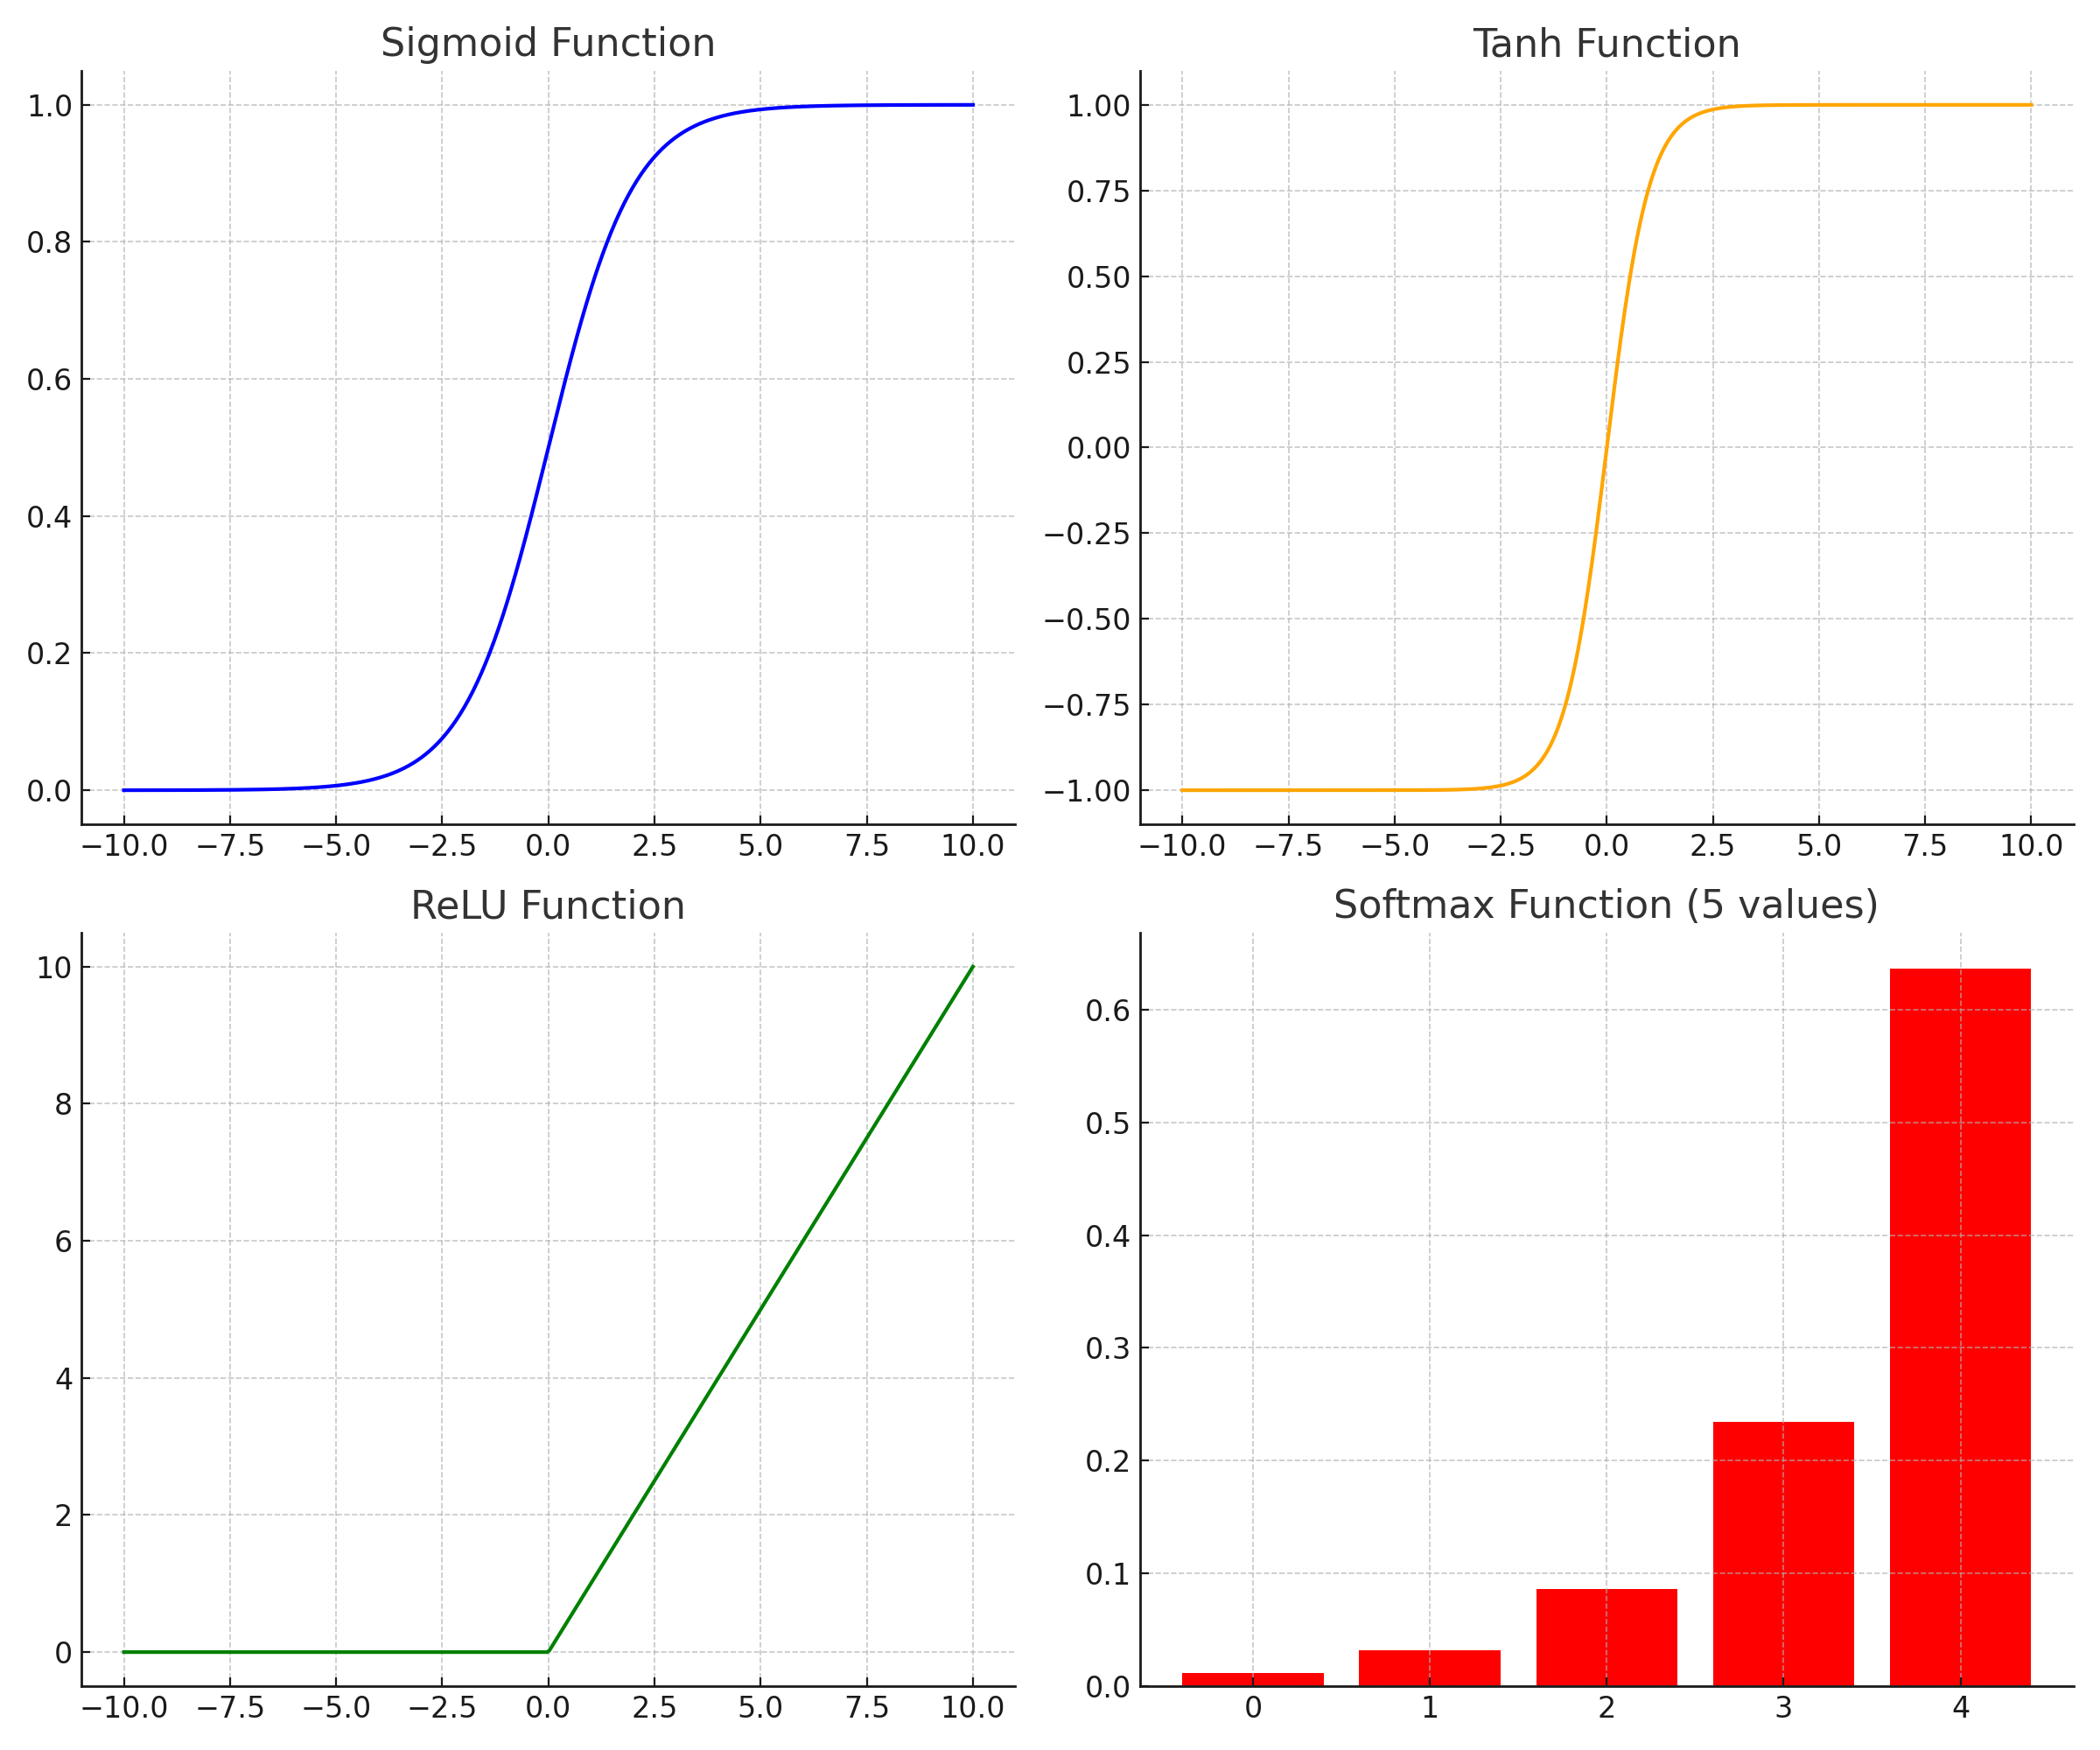
\includegraphics[width=0.9\textwidth]{assets/pics/activation_functions.png}}
    \caption{ Grafik fungsi aktivasi: (a) Sigmoid, (b) Tanh, (c) ReLU, dan (d) Softmax untuk
menunjukkan karakteristik output masing-masing fungsi}
    \source{Digenerate menggunakan Chat-GPT}
    \label{fig:activation_graph}
\end{figure}

%-----------------------------------------------------------------------------%
\section{Arsitektur Deep Learning untuk Computer Vision}
%-----------------------------------------------------------------------------%

\textit{Computer vision} merupakan domain yang telah mengalami transformasi revolusioner dengan kemunculan \textit{deep learning}. Arsitektur yang dirancang khusus untuk memproses data visual telah mencapai tingkat kinerja yang melampaui kemampuan manusia dalam banyak tugas. Dalam konteks deteksi \textit{deepfake}, pemilihan arsitektur yang tepat menjadi krusial karena setiap arsitektur memiliki bias induktif yang berbeda dalam memproses informasi visual.

\subsection{Convolutional Neural Networks (CNN)}

\textit{Convolutional Neural Networks} merepresentasikan terobosan fundamental dalam \textit{computer vision}, dirancang secara spesifik untuk mengatasi tantangan yang melekat dalam pemrosesan data visual \cite{lecun1998gradient}. Berbeda dengan jaringan \textit{fully connected} yang memperlakukan setiap piksel secara independen, CNN memanfaatkan struktur spasial dari citra melalui operasi konvolusi yang mempertahankan hubungan spasial antar piksel.

Inspirasi CNN berasal dari sistem visual biologis, khususnya konsep \textit{receptive fields} dimana neuron dalam korteks visual hanya merespons stimuli dalam wilayah spasial terbatas. Prinsip ini ditranslasikan menjadi operasi konvolusi dimana filter berukuran kecil (biasanya 3×3 atau 5×5 piksel) bergerak melintasi seluruh citra, mengekstrak fitur lokal pada setiap posisi.

Operasi konvolusi fundamental dapat diformulasikan sebagai:
\begin{equation}
(I * K)(i,j) = \sum_{m} \sum_{n} I(i+m, j+n) \cdot K(m,n)
\label{eq:convolution}
\end{equation}

dimana $I$ adalah citra masukan, $K$ adalah kernel/filter, dan $*$ mennotasikan operasi konvolusi. Setiap filter belajar mendeteksi pola spesifik seperti tepi, tekstur, atau bentuk.

\begin{figure}[H]
    \centering
    \fbox{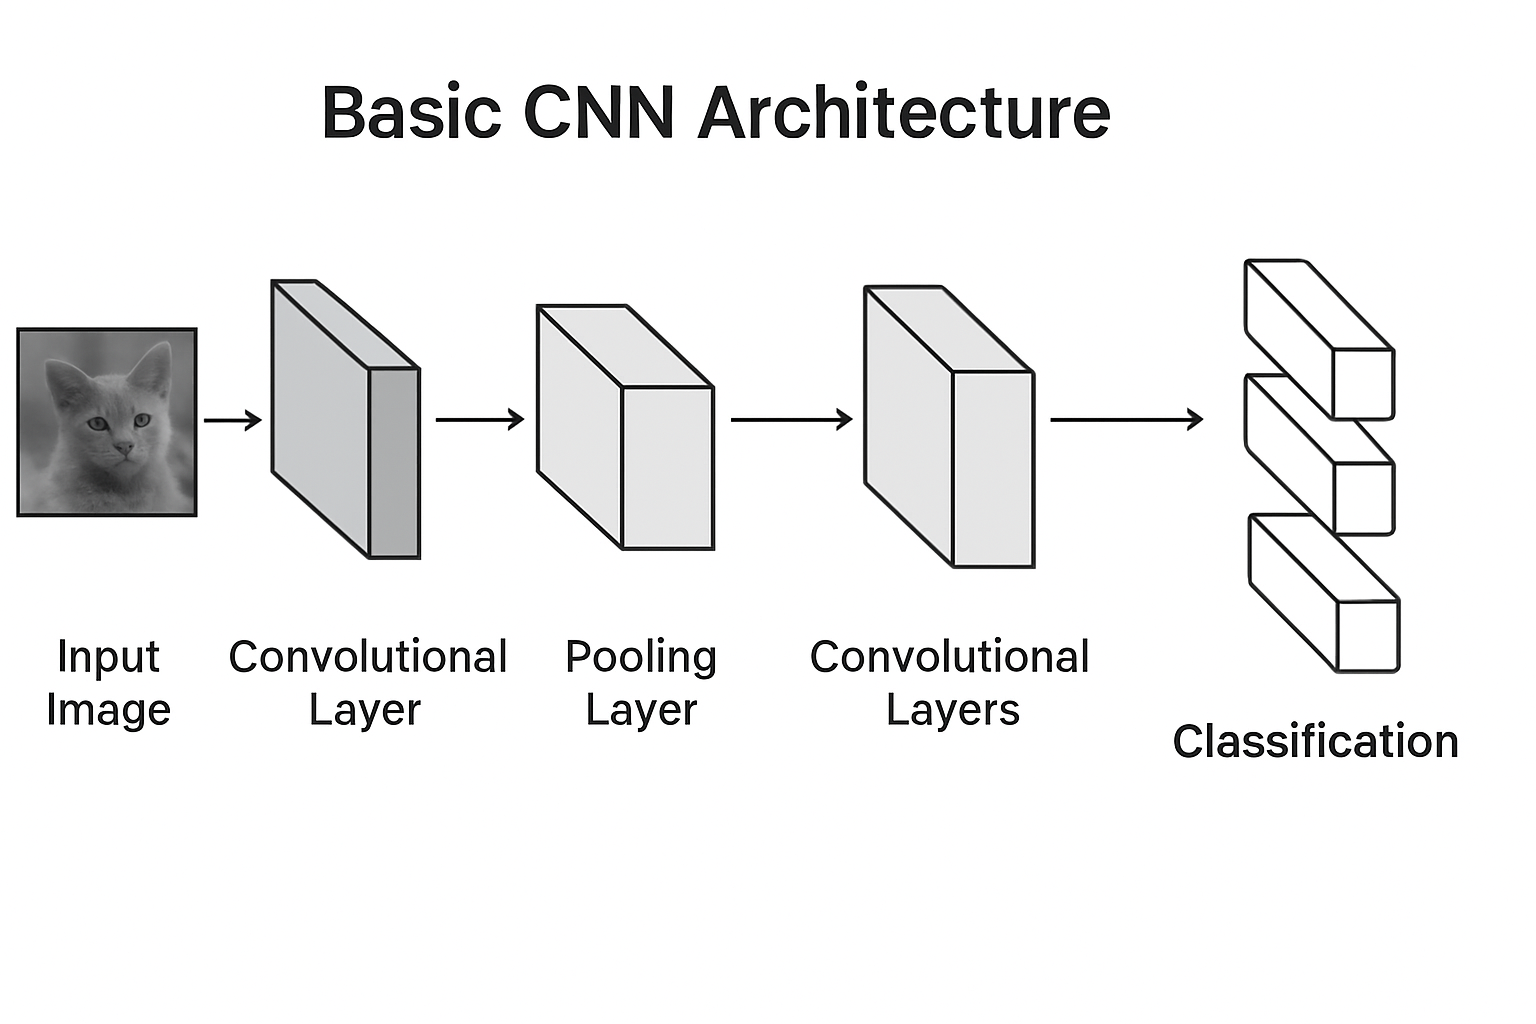
\includegraphics[width=0.9\textwidth]{assets/pics/cnn_architecture.png}}
    \caption{Arsitektur dasar CNN menunjukkan progres hierarkis dari fitur tingkat rendah ke representasi tingkat tinggi melalui lapisan konvolusi dan \textit{pooling} yang bergantian}
    \source{Diadaptasi dari \cite{lecun1998gradient}}
    \label{fig:cnn_architecture}
\end{figure}

Arsitektur CNN membangun representasi hierarkis melalui lapisan yang bergantian. \textit{Lapisan konvolusi} mengekstrak fitur lokal menggunakan filter yang dipelajari, dengan setiap filter mengkhususkan diri dalam mendeteksi pola tertentu. \textit{Lapisan pooling} mengurangi dimensi spasial sambil mempertahankan informasi penting, memberikan invariansi translasi dan efisiensi komputasi. \textit{Lapisan fully connected} pada akhir jaringan mengintegrasikan fitur yang diekstrak untuk keputusan klasifikasi akhir.

Keunggulan fundamental CNN dibandingkan jaringan \textit{fully connected} meliputi aspek-aspek krusial. \textit{Parameter sharing} memungkinkan filter yang sama digunakan di seluruh citra, secara dramatis mengurangi jumlah parameter yang perlu dipelajari. \textit{Translation invariance} memungkinkan deteksi fitur pada berbagai posisi dalam citra, krusial untuk pengenalan objek yang robust. \textit{Local connectivity} memastikan setiap neuron hanya terhubung ke wilayah spasial terbatas, menangkap pola lokal secara efektif. \textit{Hierarchical feature learning} membangun pemahaman progresif dari tepi dan tekstur tingkat rendah menuju konsep semantik tingkat tinggi.

Dalam konteks deteksi \textit{deepfake}, properti-properti ini sangat berharga karena artefak manipulasi dapat muncul pada berbagai skala dan lokasi dalam citra, dan pemrosesan hierarkis CNN dapat menangkap inkonsistensi pada berbagai tingkat abstraksi.

\subsection{Arsitektur CNN Modern}

Evolusi arsitektur CNN telah didorong oleh kebutuhan untuk mengatasi keterbatasan dari arsitektur sebelumnya sambil meningkatkan kinerja dan efisiensi. Setiap inovasi dalam arsitektur CNN modern mengatasi tantangan spesifik yang ditemukan dalam praktik, menciptakan ekosistem yang kaya dari pilihan arsitektur untuk berbagai aplikasi.

\subsubsection{ResNet: Revolusi Jaringan Dalam melalui Residual Learning}

\textit{Residual Network} (ResNet) merepresentasikan pergeseran paradigma fundamental dalam desain jaringan dalam, mengatasi salah satu hambatan utama dalam pelatihan jaringan yang sangat dalam: masalah \textit{vanishing gradient} \cite{he2016deep}. Sebelum ResNet, ada paradoks dimana menambahkan lebih banyak lapisan seharusnya tidak menurunkan kinerja (karena jaringan yang lebih dalam bisa mempelajari pemetaan identitas untuk lapisan tambahan), namun dalam praktik, jaringan yang sangat dalam sering menunjukkan degradasi kinerja.

ResNet mengatasi masalah ini melalui pengenalan kerangka \textit{residual learning}. Alih-alih mempelajari pemetaan langsung $H(x)$, blok residual belajar fungsi residual $F(x) = H(x) - x$, dengan keluaran akhir:

\begin{equation}
H(x) = F(x) + x
\label{eq:residual_output}
\end{equation}

Wawasan kunci adalah bahwa mempelajari residual lebih mudah daripada mempelajari transformasi lengkap, terutama ketika fungsi optimal mendekati pemetaan identitas.

\begin{figure}[H]
    \centering
    \fbox{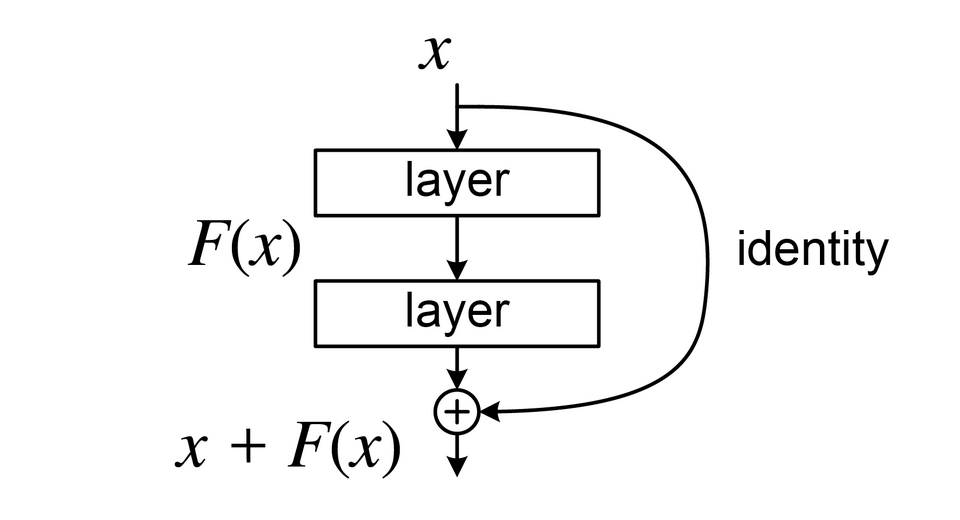
\includegraphics[width=0.6\textwidth]{assets/pics/resnet_block.png}}
    \caption{Arsitektur blok residual menunjukkan koneksi langsung yang memungkinkan aliran informasi dan propagasi gradien langsung melalui jalur pintas}
    \source{Diadaptasi dari \cite{he2016deep}}
    \label{fig:resnet_block}
\end{figure}

\textit{Skip connections} dalam ResNet berfungsi sebagai "jalan raya informasi" yang memungkinkan gradien mengalir langsung ke lapisan sebelumnya, mengurangi masalah \textit{vanishing gradient}. Hal ini memungkinkan pelatihan jaringan dengan ratusan atau bahkan ribuan lapisan, membuka kemungkinan untuk mempelajari representasi yang sangat kompleks.

Dalam konteks deteksi \textit{deepfake}, kemampuan ResNet untuk mempelajari representasi yang sangat dalam khususnya berharga karena artefak manipulasi yang halus mungkin memerlukan transformasi fitur yang kompleks untuk dideteksi secara efektif. Jaringan dalam dapat menangkap pola rumit yang mengindikasikan pembangkitan konten sintetis.

\subsubsection{Xception: Extreme Inception dan Depthwise Separable Convolutions}

\textit{Xception} merepresentasikan solusi elegan untuk efisiensi komputasi dalam desain CNN melalui interpretasi ekstrem dari hipotesis Inception \cite{chollet2017xception}. Inovasi inti terletak pada penggantian konvolusi standar dengan \textit{depthwise separable convolutions}, yang secara dramatis mengurangi biaya komputasi sambil mempertahankan atau bahkan meningkatkan kinerja.

Konvolusi standar secara simultan melakukan konvolusi spasial dan korelasi lintas saluran dalam operasi tunggal. Xception memisahkan dua operasi ini menjadi langkah berurutan yang lebih efisien. \textit{Depthwise separable convolution} memecah proses ini menjadi:

\textbf{Depthwise Convolution}: Mengaplikasikan filter spasial secara independen pada setiap saluran masukan, menangkap korelasi spasial dalam setiap saluran tanpa mencampur informasi lintas saluran.

\textbf{Pointwise Convolution}: Menggunakan konvolusi 1×1 untuk mengkombinasikan informasi lintas saluran, mempelajari kombinasi optimal saluran-wise dari fitur yang telah difilter spasial.

\begin{figure}[H]
    \centering
    \fbox{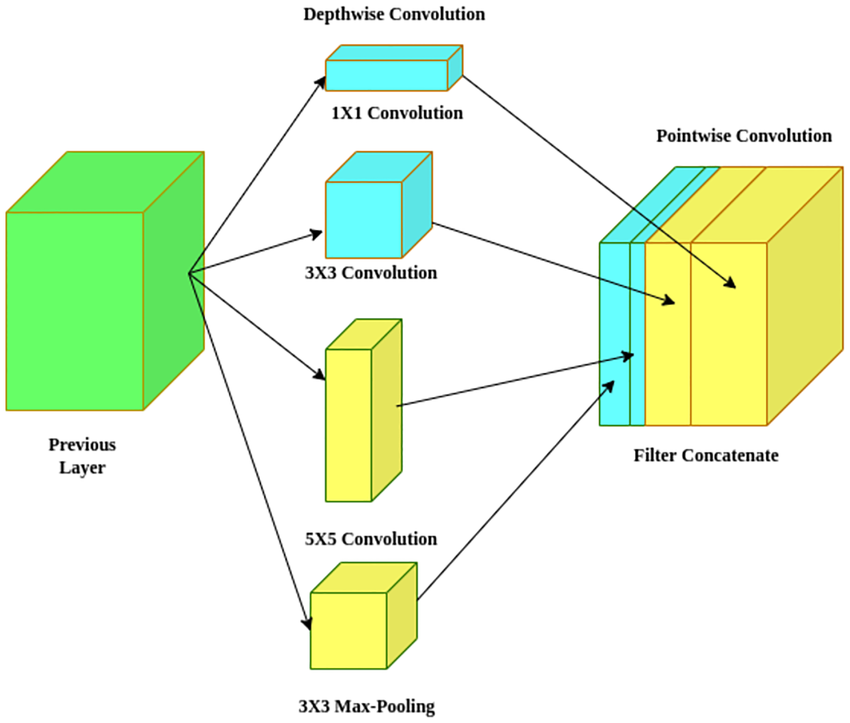
\includegraphics[width=0.8\textwidth]{assets/pics/xception_block.png}}
    \caption{Arsitektur Depthwise Separable Convolution menunjukkan pemisahan pemrosesan spasial dan saluran-wise untuk meningkatkan efisiensi}
    \source{Diadaptasi dari \cite{chollet2017xception}}
    \label{fig:xception_block}
\end{figure}

Pendekatan ini tidak hanya mengurangi kompleksitas komputasi secara signifikan (biasanya pengurangan 8-10x dalam multiply-adds) tetapi juga memberikan fleksibilitas pemodelan. Pemisahan pemrosesan spasial dan saluran memungkinkan jaringan untuk secara independen mengoptimalkan ekstraksi fitur spasial dan pencampuran saluran, berpotensi mengarah ke representasi fitur yang lebih baik.

Untuk deteksi \textit{deepfake}, pemrosesan efisien Xception khususnya menguntungkan karena memungkinkan penerapan model canggih dengan batasan komputasi, sambil mempertahankan sensitivitas tinggi untuk mendeteksi artefak manipulasi yang halus.

\subsubsection{EfficientNet: Penskalaan Berprinsip untuk Kinerja Optimal}

\textit{EfficientNet} mengatasi pertanyaan fundamental dalam desain CNN: bagaimana cara optimal untuk menskala jaringan untuk kinerja yang lebih baik \cite{tan2019efficientnet}. Pendekatan tradisional fokus pada penskalaan dimensi tunggal - membuat jaringan lebih dalam (lebih banyak lapisan), lebih lebar (lebih banyak saluran), atau memproses masukan resolusi lebih tinggi. EfficientNet memperkenalkan \textit{compound scaling} yang secara sistematis menyeimbangkan ketiga dimensi.

Wawasan inti adalah bahwa ketiga dimensi penskalaan saling bergantung. Meningkatkan resolusi masukan memerlukan lebih banyak lapisan untuk menangkap pola detail, dan lebih banyak saluran untuk menangkap kepadatan informasi yang meningkat. \textit{Compound scaling} mengkoordinasikan penskalaan di semua dimensi menggunakan pendekatan berprinsip:

\begin{align}
\text{kedalaman} &= \alpha^\phi \label{eq:depth_scaling} \\
\text{lebar} &= \beta^\phi \label{eq:width_scaling} \\
\text{resolusi} &= \gamma^\phi \label{eq:resolution_scaling}
\end{align}

dengan batasan yang memastikan biaya komputasi total berskala secara dapat diprediksi: $\alpha \cdot \beta^2 \cdot \gamma^2 \approx 2$

Koefisien $\alpha$, $\beta$, dan $\gamma$ ditentukan melalui pencarian grid sistematis pada jaringan dasar, kemudian $\phi$ digunakan sebagai koefisien majemuk untuk memperbesar jaringan secara seragam.

\begin{figure}[H]
    \centering
    \fbox{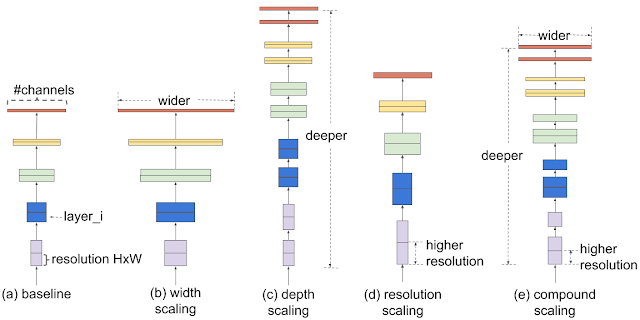
\includegraphics[width=0.9\textwidth]{assets/pics/efficientnet_scaling.png}}
    \caption{Perbandingan strategi penskalaan menunjukkan superioritas compound scaling dalam mencapai tradeoff akurasi-efisiensi yang optimal}
    \source{Diadaptasi dari \cite{tan2019efficientnet}}
    \label{fig:efficientnet_scaling}
\end{figure}

Hasil dari pendekatan ini adalah keluarga model yang secara konsisten mencapai akurasi \textit{state-of-the-art} dengan parameter dan FLOP yang signifikan lebih sedikit dibandingkan pendekatan penskalaan tradisional. EfficientNet menunjukkan bahwa perhatian yang cermat terhadap strategi penskalaan dapat menghasilkan peningkatan dramatis dalam efisiensi tanpa mengorbankan kinerja.

Dalam aplikasi deteksi \textit{deepfake}, pendekatan seimbang EfficientNet khususnya berharga karena memberikan tradeoff optimal antara akurasi deteksi dan efisiensi komputasi, memungkinkan penerapan dalam skenario praktis dengan batasan sumber daya.

%-----------------------------------------------------------------------------%
\section{Ensemble Learning dan Weighted Averaging}
%-----------------------------------------------------------------------------%

\textit{Ensemble learning} merepresentasikan salah satu paradigma paling powerful dalam \textit{machine learning}, berdasarkan intuisi fundamental bahwa kombinasi dari beberapa prediktor independen seringkali superior dibandingkan prediktor individual manapun. Prinsip ini, yang dikenal sebagai \textit{"wisdom of crowds"}, telah terbukti efektif di berbagai aplikasi dan khususnya relevan untuk tugas yang menantang seperti deteksi \textit{deepfake} dimana model tunggal mungkin memiliki bias atau titik buta \cite{dietterich2000ensemble}.

\subsection{Prinsip Dasar dan Fondasi Teoritis}

Fondasi teoritis dari \textit{ensemble learning} berakar pada teori pembelajaran statistik, khususnya konsep dekomposisi bias-varians. Pemahaman ini krusial untuk mengapresiasi mengapa metode ensemble bekerja dan kapan mereka diharapkan memberikan peningkatan dibanding model individual.

Keberhasilan ensemble dapat dijelaskan melalui lensa \textit{bias-variance tradeoff} \cite{breiman1996bias}. Untuk tugas regresi, galat yang diharapkan dari prediktor dapat didekomposisi menjadi tiga komponen: bias (galat sistematis dari asumsi yang salah), varians (sensitivitas terhadap fluktuasi kecil dalam set pelatihan), dan galat yang tidak dapat direduksi (noise yang melekat dalam masalah).

Ketika kita mengkombinasikan beberapa model yang dilatih pada data berbeda atau dengan algoritma berbeda, ensemble dapat secara simultan mengurangi varians tanpa harus meningkatkan bias. Untuk ensemble dari $M$ model yang tidak berkorelasi dengan varians yang sama $\sigma^2$, varians dari prediksi ensemble berkurang menjadi:

\begin{equation}
\text{Var}[\bar{f}(x)] = \frac{\sigma^2}{M}
\label{eq:ensemble_variance}
\end{equation}

Pengurangan ini powerful, tetapi efektivitasnya sangat bergantung pada diversitas antar anggota ensemble. Jika model sangat berkorelasi (membuat kesalahan serupa), manfaat dari ensembling berkurang signifikan.

\textbf{Diversitas} merupakan kunci keberhasilan \textit{ensemble learning}. Model yang berbeda cenderung membuat kesalahan yang berbeda pada instans yang berbeda, dan ketika galat tidak berkorelasi atau berkorelasi negatif, mereka dapat saling membatalkan ketika dikombinasikan. Dalam konteks deteksi \textit{deepfake}, arsitektur CNN yang berbeda menangkap jenis informasi visual dan artefak yang berbeda, menciptakan diversitas alami yang menguntungkan untuk kinerja ensemble.

\begin{figure}[H]
    \centering
    \fbox{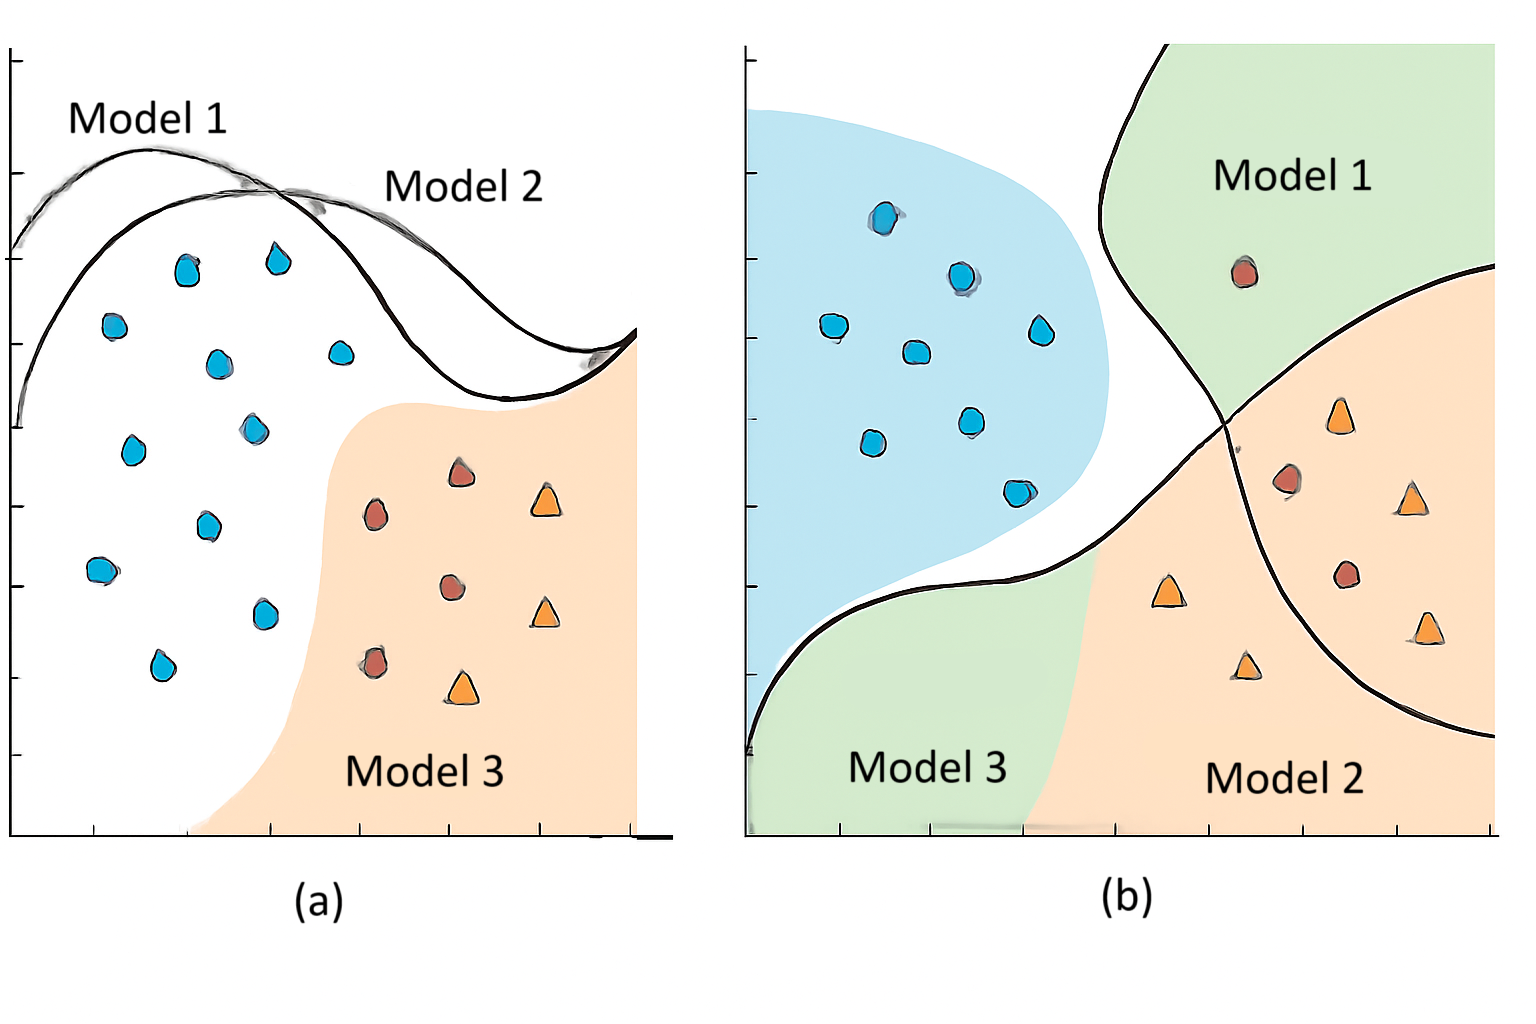
\includegraphics[width=0.8\textwidth]{assets/pics/ensemble_diversity.png}}
    \caption{Visualisasi efek diversitas ensemble: pola galat yang beragam memungkinkan koreksi galat mutual, sementara pola galat yang serupa memberikan manfaat ensemble yang minimal}
    \source{Ilustrasi berdasarkan \cite{brown2005diversity}}
    \label{fig:ensemble_diversity}
\end{figure}

Diversitas dapat diukur melalui berbagai metrik. Q-statistic mengukur tingkat kesepakatan antar classifier, ukuran ketidaksepakatan menghitung proporsi instans dimana classifier tidak setuju, dan ukuran kesalahan ganda mengukur proporsi instans dimana kedua classifier salah. Ensemble optimal menyeimbangkan akurasi individual dengan diversitas antar model.

\subsection{Metode Ensemble Learning: Tinjauan Komprehensif}

Lanskap metode ensemble kaya dan beragam, dengan setiap pendekatan menargetkan aspek berbeda dari konstruksi dan kombinasi ensemble. Memahami paradigma ensemble yang berbeda esensial untuk memilih metode yang tepat untuk aplikasi spesifik.

\subsubsection{Bagging: Bootstrap Aggregating untuk Pengurangan Varians}

\textit{Bootstrap Aggregating} (Bagging) mengatasi komponen varians dari galat prediksi melalui pelatihan beberapa model pada sampel bootstrap yang berbeda dari data pelatihan \cite{breiman1996bagging}. Pendekatan ini khususnya efektif untuk model dengan varians tinggi seperti \textit{decision trees}, tetapi juga dapat diterapkan untuk jaringan saraf.

Ide inti di balik bagging adalah bahwa merata-ratakan prediksi dari beberapa model yang dilatih pada dataset yang sedikit berbeda dapat mengurangi varians keseluruhan tanpa secara signifikan mempengaruhi bias. \textit{Bootstrap sampling} menciptakan set pelatihan yang beragam dengan mengambil sampel ulang data asli dengan penggantian, memastikan bahwa setiap model melihat versi data yang sedikit berbeda.

Proses dimulai dengan menghasilkan $M$ sampel bootstrap, masing-masing berukuran sama dengan set pelatihan asli tetapi dengan komposisi berbeda karena pengambilan sampel dengan penggantian. Setiap sampel bootstrap kemudian digunakan untuk melatih model terpisah. Prediksi akhir diperoleh melalui perata-rataan (untuk regresi) atau \textit{majority voting} (untuk klasifikasi):

\begin{equation}
\hat{y} = \text{mode}\{h_1(x), h_2(x), \ldots, h_M(x)\}
\label{eq:bagging_prediction}
\end{equation}

Bagging khususnya efektif ketika model dasar rentan terhadap \textit{overfitting}, karena efek perata-rataan menghaluskan keanehan model individual. Dalam konteks \textit{deep learning}, bagging dapat diterapkan dengan melatih arsitektur yang sama pada subset data yang berbeda atau dengan inisialisasi acak yang berbeda.

\subsubsection{Boosting: Pembelajaran Berurutan dengan Fokus Galat}

\textit{Boosting} mengambil pendekatan yang secara fundamental berbeda dibandingkan bagging, fokus pada pengurangan bias melalui proses pelatihan berurutan dimana setiap model berikutnya fokus pada memperbaiki galat yang dibuat oleh model sebelumnya \cite{freund1997decision}. Ini menciptakan proses pembelajaran adaptif yang secara progresif meningkatkan kinerja pada instans yang sulit.

\textit{AdaBoost} (Adaptive Boosting) merupakan algoritma boosting seminal yang mengilustrasikan prinsip inti. Algoritma mempertahankan bobot untuk setiap instans pelatihan, awalnya diatur sama. Setelah melatih setiap \textit{weak learner}, bobot instans diperbarui: instans yang diklasifikasikan dengan benar menerima bobot yang lebih rendah, sementara instans yang salah diklasifikasikan menerima bobot yang lebih tinggi. Skema pembobotan ini memastikan bahwa \textit{learner} berikutnya memfokuskan perhatian pada instans yang sebelumnya sulit.

Sifat berurutan dari boosting menciptakan kombinasi yang kuat dimana ensemble akhir menggabungkan \textit{weak learner} secara berbobot, dengan performer yang lebih baik menerima pengaruh yang lebih tinggi dalam keputusan akhir. Formulasi matematis memastikan bahwa galat pelatihan menurun secara eksponensial dengan jumlah putaran boosting, di bawah kondisi yang tepat.

Namun, boosting dapat rentan terhadap \textit{overfitting} dan noise, terutama dengan model yang sangat dalam seperti CNN. Regularisasi yang hati-hati dan \textit{early stopping} seringkali diperlukan ketika menerapkan prinsip boosting untuk aplikasi \textit{deep learning}.

\subsubsection{Stacking: Meta-Learning untuk Kombinasi Optimal}

\textit{Stacking} (Stacked Generalization) merepresentasikan pendekatan canggih untuk kombinasi ensemble melalui pengenalan \textit{meta-learner} yang mempelajari cara optimal untuk mengkombinasikan prediksi model dasar \cite{wolpert1992stacked}. Tidak seperti bagging atau boosting yang menggunakan aturan kombinasi sederhana, stacking mempelajari fungsi kombinasi dari data.

Arsitektur terdiri dari dua tingkat: \textit{Level-0 base learners} dilatih pada data asli, dan \textit{Level-1 meta-learner} dilatih untuk mengkombinasikan prediksi Level-0. Proses biasanya melibatkan \textit{cross-validation} untuk menghasilkan meta-fitur: model dasar dilatih pada subset data digunakan untuk menghasilkan prediksi untuk bagian yang ditahan, menciptakan set pelatihan untuk \textit{meta-learner}.

Stacking khususnya powerful karena \textit{meta-learner} dapat mempelajari kombinasi non-linear yang kompleks dari prediksi dasar, berpotensi menemukan efek interaksi dan kekuatan komplementer antar model dasar. Namun, kompleksitas pendekatan stacking memerlukan validasi yang hati-hati untuk menghindari \textit{overfitting}, terutama dengan data pelatihan yang terbatas.

\subsection{Weighted Averaging: Kesederhanaan Elegan dengan Efektivitas Terbukti}

\textit{Weighted averaging} merepresentasikan titik manis dalam metodologi ensemble - cukup canggih untuk menangkap kinerja diferensial antar model dasar, namun cukup sederhana untuk diimplementasikan secara andal dan diinterpretasikan secara bermakna \cite{kuncheva2004combining}. Metode ini memberikan bobot berbeda kepada prediksi model dasar berdasarkan estimasi kinerja, menciptakan kombinasi bernuansa yang memanfaatkan kekuatan model yang lebih baik sambil tetap mendapat manfaat dari diversitas model yang lebih lemah.

Formulasi matematis yang sederhana namun powerful:
\begin{equation}
\hat{y}_{ensemble}(x) = \sum_{i=1}^{N} w_i \cdot \hat{y}_i(x)
\label{eq:weighted_ensemble}
\end{equation}

dengan batasan fundamental: $\sum_{i=1}^{N} w_i = 1$ dan $w_i \geq 0$. Batasan ini memastikan bahwa keluaran ensemble tetap dalam batas yang wajar dan bahwa semua model berkontribusi secara non-negatif.

\textbf{Strategi Pembobotan Berbasis Kinerja} yang diadopsi dalam penelitian ini memberikan bobot proporsional terhadap kinerja validasi:
\begin{equation}
w_i = \frac{\text{performance}_i}{\sum_{j=1}^{N} \text{performance}_j}
\label{eq:performance_weight}
\end{equation}

Pendekatan ini intuitif dan praktis efektif: model yang menunjukkan kinerja superior pada data validasi menerima pengaruh yang sesuai lebih tinggi dalam keputusan ensemble. Strategi ini mengasumsikan bahwa kinerja validasi prediktif terhadap kinerja tes, asumsi yang wajar ketika set validasi representatif dari distribusi target.

\begin{figure}[H]
    \centering
    \fbox{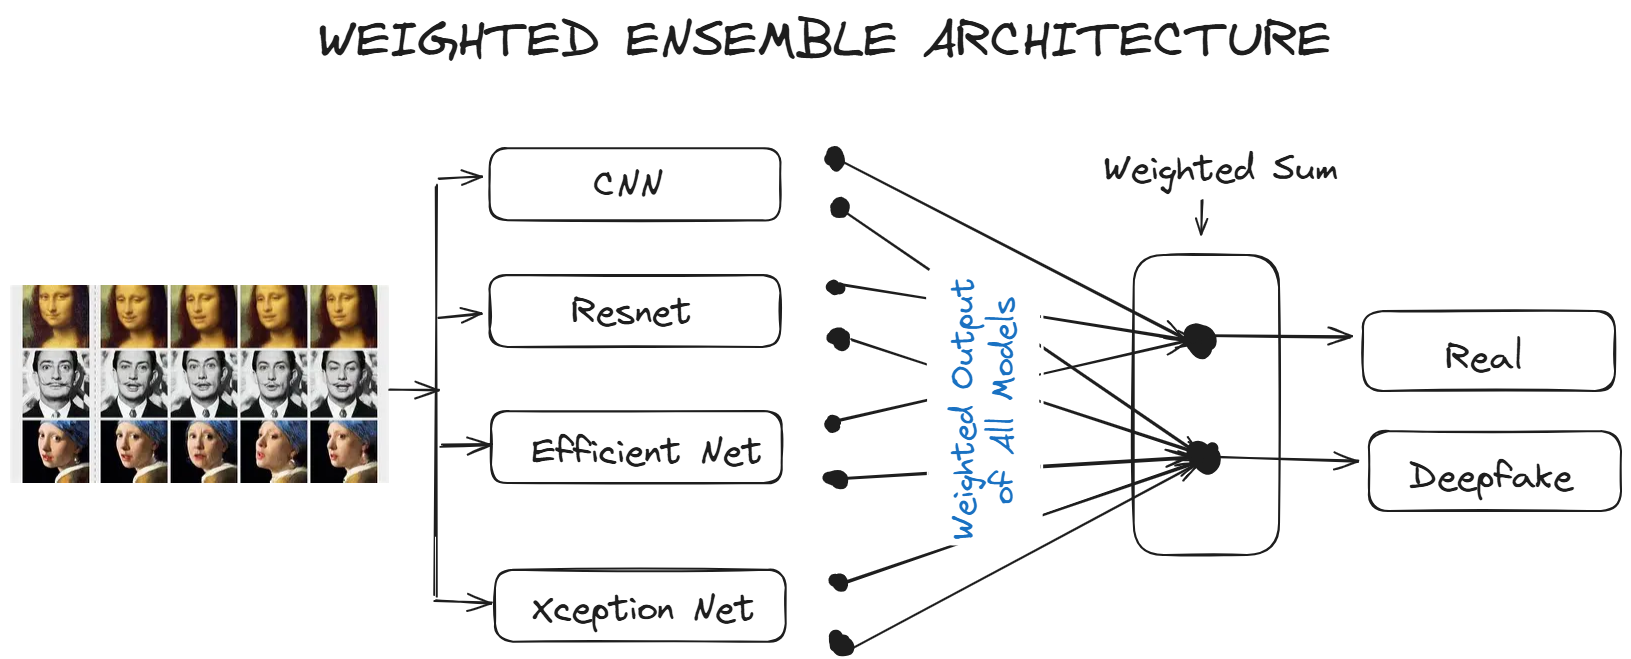
\includegraphics[width=0.9\textwidth]{assets/pics/weighted_ensemble.png}}
    \caption{Arsitektur ensemble berbobot menunjukkan aliran informasi dari masukan melalui beberapa model dasar, kombinasi berbobot, dan prediksi akhir}
    \source{Ilustrasi berdasarkan metodologi penelitian}
    \label{fig:weighted_ensemble}
\end{figure}

Keunggulan \textit{weighted averaging} meliputi beberapa aspek krusial. \textbf{Kesederhanaan komputasi} memungkinkan implementasi efisien tanpa prosedur pelatihan yang kompleks. \textbf{Interpretabilitas} memungkinkan pemahaman mudah tentang kontribusi setiap model terhadap keputusan akhir. \textbf{Fleksibilitas} dalam pemberian bobot memungkinkan adaptasi terhadap metrik kinerja yang berbeda atau persyaratan spesifik domain. \textbf{Robustness} terhadap kegagalan model individual, karena model dengan kinerja buruk secara otomatis menerima pengaruh yang lebih rendah.

Dalam konteks deteksi \textit{deepfake}, \textit{weighted averaging} khususnya cocok karena arsitektur CNN yang berbeda menunjukkan kinerja yang bervariasi pada jenis artefak manipulasi yang berbeda. Pemberian bobot berdasarkan akurasi validasi memastikan bahwa model dengan kemampuan deteksi superior memberikan pengaruh yang tepat pada keputusan ensemble akhir.

%-----------------------------------------------------------------------------%
\section{Teknologi Deepfake dan Deteksi}
%-----------------------------------------------------------------------------%

Era digital modern telah menyaksikan kemunculan teknologi manipulasi media canggih yang menantang konsep tradisional tentang kebenaran visual. Teknologi \textit{deepfake}, yang menggabungkan kekuatan \textit{deep learning} dengan aksesibilitas alat tingkat konsumen, merepresentasikan pergeseran paradigma dalam lanskap pembuatan dan manipulasi media digital. Memahami teknologi ini - baik dalam kemampuan maupun keterbatasannya - esensial untuk mengembangkan langkah-langkah perlawanan yang efektif.

\subsection{Teknologi Deepfake: Evolusi dan Keadaan Saat Ini}

Teknologi \textit{deepfake}, nama yang berasal dari penggabungan "\textit{deep learning}" dan "\textit{fake}", merepresentasikan konvergensi dari beberapa kemajuan teknologi dalam kecerdasan buatan, \textit{computer vision}, dan pemrosesan media \cite{rana2022deepfake}. Teknologi ini secara fundamental memanfaatkan kekuatan \textit{Generative Adversarial Networks} (GANs) untuk menciptakan konten media sintetis yang sangat realistis, khususnya untuk aplikasi penukaran wajah dan reenaktmen wajah.

Lintasan historis teknologi \textit{deepfake} luar biasa dalam kecepatan perkembangan yang pesat. Teknologi pertama kali mendapat perhatian luas pada akhir 2017 ketika pengguna Reddit dengan nama pengguna "deepfakes" merilis kode sumber terbuka untuk penukaran wajah menggunakan framework \textit{deep learning} yang tersedia \cite{ajder2019deepfakes}. Implementasi awal masih kasar, menghasilkan hasil dengan artefak yang jelas dan memerlukan keahlian teknis yang substansial untuk penerapan.

Perkembangan teknologi ini dapat ditelusuri melalui fase evolusi yang berbeda. Sistem \textbf{Generasi 1} berbasis pada arsitektur autoencoder sederhana, menghasilkan keluaran resolusi rendah dengan artefak visual yang jelas. \textbf{Generasi 2} memperkenalkan pendekatan berbasis GAN dengan peningkatan kualitas yang signifikan, memungkinkan pembuatan konten palsu yang lebih meyakinkan. Sistem \textbf{Generasi 3} memanfaatkan arsitektur canggih seperti StyleGAN dan teknik \textit{progressive growing}, mencapai kualitas yang mendekati fotorealistis. Sistem \textbf{Generasi 4} saat ini memungkinkan generasi real-time dan reenaktmen wajah dengan persyaratan komputasi minimal.

Teknologi \textit{deepfake} kontemporer menunjukkan kemampuan canggih yang mencakup beberapa modalitas. Sistem reenaktmen wajah dapat memanipulasi ekspresi wajah dan gerakan kepala secara real-time, memungkinkan peniruan yang meyakinkan untuk panggilan video atau live stream. Teknologi sintesis suara dapat mereplikasi pola bicara dengan fidelitas yang luar biasa menggunakan jumlah audio target yang relatif kecil. Sistem puppeteering seluruh tubuh dapat mentransfer gerakan dan gestur tubuh, menciptakan kemampuan peniruan yang komprehensif.

\textbf{Aplikasi Positif} dari teknologi \textit{deepfake} menunjukkan potensi signifikan untuk penggunaan yang bermanfaat. Industri hiburan memanfaatkan teknologi untuk kebangkitan digital aktor yang telah meninggal, memungkinkan penyelesaian film atau pembuatan konten baru yang menampilkan performer terkasih. Aplikasi pendidikan termasuk simulasi tokoh sejarah, memungkinkan siswa berinteraksi dengan representasi virtual dari kepribadian sejarah penting. Aplikasi aksesibilitas menyediakan sintesis suara untuk individu dengan gangguan bicara, memulihkan kemampuan komunikasi. Seni kreatif mendapat manfaat dari penangkapan kinerja yang ditingkatkan dan pembuatan avatar digital.

Namun, \textbf{risiko dan ancaman} yang terkait dengan teknologi \textit{deepfake} sama signifikan dan mengkhawatirkan. Kampanye disinformasi dapat memanfaatkan konten palsu yang realistis untuk manipulasi politik atau serangan rekayasa sosial. Aplikasi penipuan identitas memungkinkan peniruan yang tidak sah untuk penipuan keuangan atau kerusakan reputasi. Pelanggaran privasi melalui pembuatan citra intim tanpa persetujuan merepresentasikan kekhawatiran etis dan hukum yang serius. Serangan rekayasa sosial yang ditingkatkan dapat memanfaatkan peniruan yang meyakinkan untuk spionase korporat atau manipulasi personal.

\begin{figure}[H]
    \centering
    \fbox{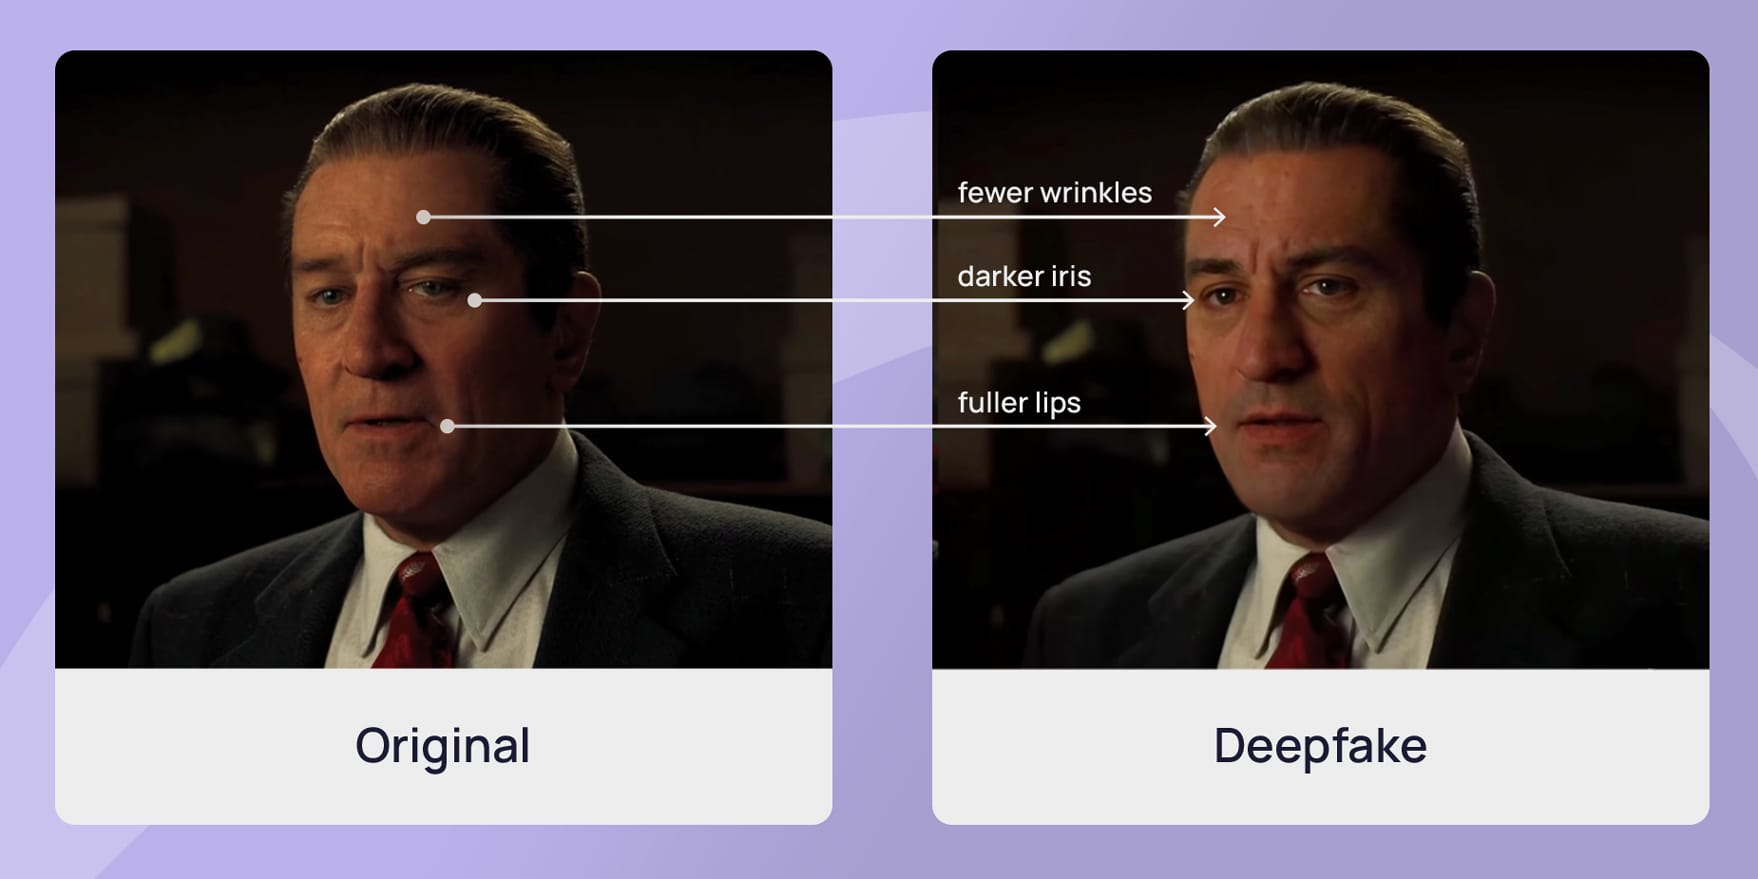
\includegraphics[width=0.9\textwidth]{assets/pics/deepfake_examples.jpg}}
    \caption{Pengaplikasian Deepfake}
    \source{Sumber: DQLab}
    \label{fig:deepfake_examples}
\end{figure}

\subsection{Generative Adversarial Networks: Mesin Pembuatan Media Sintetis}

\textit{Generative Adversarial Networks} merupakan fondasi teknologi yang memungkinkan pembuatan \textit{deepfake} canggih, merepresentasikan terobosan dalam pemodelan generatif yang merevolusi kemampuan untuk menciptakan konten sintetis \cite{goodfellow2014generative}. Memahami arsitektur dan dinamika pelatihan GAN krusial untuk memahami baik kemampuan maupun potensi kerentanan teknologi \textit{deepfake}.

Kerangka GAN terdiri dari dua jaringan saraf yang terlibat dalam proses pelatihan adversarial: jaringan generator yang berusaha menciptakan konten sintetis yang realistis, dan jaringan discriminator yang mencoba membedakan antara konten nyata dan yang dihasilkan. Hubungan adversarial ini menciptakan lingkungan pelatihan dinamis dimana kedua jaringan terus meningkat sebagai respons terhadap kemampuan lawan.

Formulasi matematis inti dari tujuan pelatihan GAN menangkap esensi hubungan adversarial:
\begin{equation}
\min_G \max_D V(D,G) = \mathbb{E}_{x \sim p_{data}}[\log D(x)] + \mathbb{E}_{z \sim p_z}[\log(1-D(G(z)))]
\label{eq:gan_objective}
\end{equation}

Discriminator memaksimalkan kemampuan untuk mengklasifikasikan sampel nyata dan palsu dengan benar, sementara generator meminimalkan akurasi klasifikasi discriminator. Proses pelatihan berlanjut hingga keseimbangan Nash tercapai, secara teoritis menghasilkan generator yang menghasilkan sampel yang tidak dapat dibedakan dari data nyata.

\begin{figure}[H]
    \centering
    \fbox{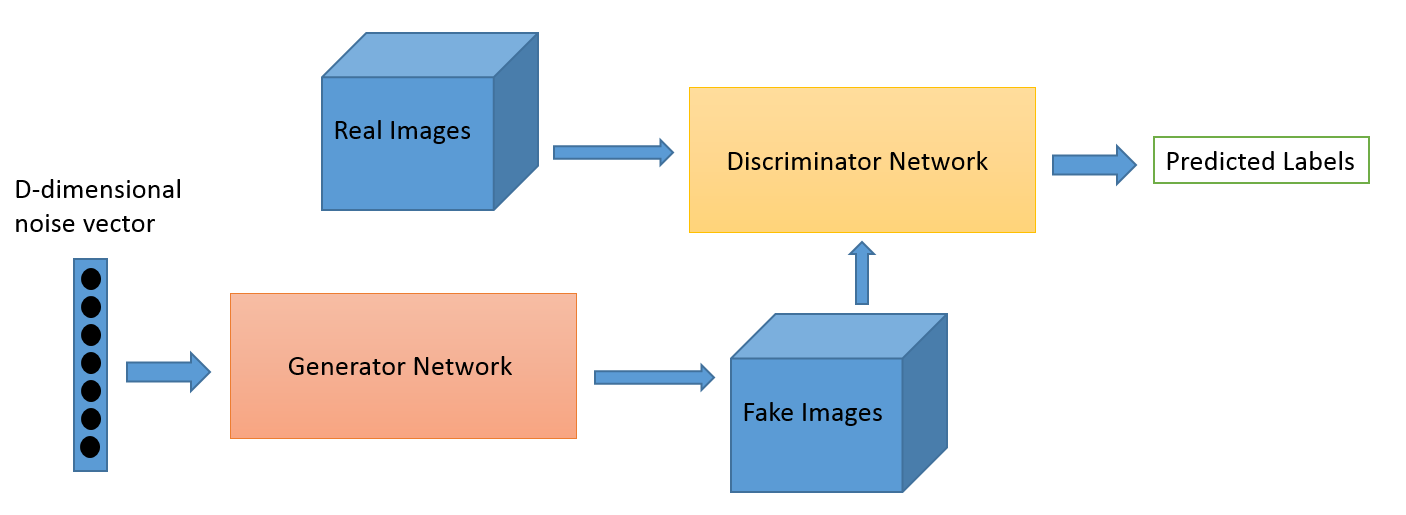
\includegraphics[width=0.9\textwidth]{assets/pics/gan_architecture.png}}
    \caption{Tinjauan arsitektur GAN menunjukkan setup pelatihan adversarial: (a) Fase pelatihan dengan fungsi kerugian kompetitif, (b) Arsitektur generator untuk pembuatan konten sintetis, (c) Arsitektur discriminator untuk klasifikasi keaslian}
    \source{Diadaptasi dari \cite{goodfellow2014generative}}
    \label{fig:gan_architecture}
\end{figure}

Dinamika pelatihan GAN khususnya kompleks karena melibatkan optimisasi simultan dari dua jaringan dengan tujuan yang bertentangan. \textbf{Pelatihan discriminator} fokus pada memaksimalkan akurasi klasifikasi antara sampel nyata dan sintetis, mempelajari fitur yang semakin canggih untuk mendeteksi konten yang dihasilkan. \textbf{Pelatihan generator} mengoptimalkan untuk menipu discriminator, belajar menghasilkan konten sintetis yang meniru properti statistik data nyata.

Beberapa varian arsitektur GAN dasar telah dikembangkan untuk meningkatkan stabilitas pelatihan dan kualitas keluaran. \textbf{DCGAN} memperkenalkan pedoman arsitektur yang dioptimalkan untuk generasi gambar, termasuk penggunaan konvolusi bergeser, normalisasi batch, dan fungsi aktivasi spesifik. \textbf{StyleGAN} memungkinkan kontrol fine-grained atas konten yang dihasilkan melalui pendekatan generasi berbasis gaya, memungkinkan manipulasi atribut wajah spesifik secara independen. \textbf{CycleGAN} memungkinkan translasi gambar-ke-gambar yang tidak berpasangan, memfasilitasi aplikasi transfer domain.

Tantangan pelatihan dalam GAN termasuk \textit{mode collapse} (generator menghasilkan variasi keluaran yang terbatas), ketidakstabilan pelatihan (perilaku osilasi daripada konvergensi), dan \textit{vanishing gradients} (generator menerima umpan balik yang tidak informatif). Mengatasi tantangan ini memerlukan desain arsitektur yang hati-hati, modifikasi prosedur pelatihan, dan seringkali optimisasi spesifik domain.

\subsection{Deteksi Deepfake sebagai Tantangan Binary Classification}

Merumuskan deteksi \textit{deepfake} sebagai tugas \textit{binary classification} memberikan kerangka yang jelas untuk mendekati masalah secara sistematis, namun kompleksitas tugas meluas jauh melampaui tantangan klasifikasi tradisional \cite{verdoliva2020media}. Memahami karakteristik unik deteksi \textit{deepfake} esensial untuk mengembangkan langkah-langkah perlawanan yang efektif.

\textbf{Target Adversarial yang Berkembang} merepresentasikan tantangan fundamental yang membedakan deteksi \textit{deepfake} dari tugas klasifikasi statis. Generator \textit{deepfake} terus berkembang, dengan arsitektur dan teknik pelatihan baru menghasilkan konten sintetis dengan pola artefak yang berbeda. Sistem deteksi oleh karena itu harus mempertahankan efektivitas terhadap teknik generasi masa depan yang tidak diketahui, memerlukan kemampuan generalisasi yang robust melampaui skenario \textit{machine learning} tradisional.

Deteksi \textit{deepfake} kontemporer menghadapi dinamika perlombaan senjata dimana peningkatan dalam kualitas generasi mendorong kemajuan yang sesuai dalam kecanggihan deteksi. Evolusi adversarial ini menciptakan target bergerak yang memerlukan strategi deteksi adaptif daripada penerapan model tetap.

\textbf{Deteksi Artefak Halus} memerlukan sensitivitas ekstrem terhadap inkonsistensi kecil yang mungkin mengindikasikan pembuatan konten sintetis. Artefak ini termanifestasi di berbagai domain dan skala, memerlukan pendekatan analisis yang komprehensif.

\textit{Artefak domain spasial} termasuk inkonsistensi dalam model pencahayaan, proyeksi bayangan, refleksi di mata atau permukaan reflektif lainnya, ketidakteraturan tekstur kulit, dan artefak batas di sekitar wilayah yang dimanipulasi. Artefak ini seringkali halus dan mungkin memerlukan analisis resolusi tinggi untuk deteksi yang andal.

\textit{Artefak domain temporal} muncul dalam urutan video, termasuk pola gerakan kepala yang tidak alami, frekuensi kedipan mata yang tidak teratur, dinamika ekspresi wajah yang tidak konsisten, dan diskontinuitas temporal dalam pelacakan fitur wajah. Analisis konsistensi temporal memberikan petunjuk yang kuat untuk mendeteksi konten video yang dimanipulasi.

\textit{Artefak domain frekuensi} hasil dari proses generasi GAN, menciptakan tanda tangan spektral yang khas yang mungkin dapat dideteksi melalui analisis Fourier atau dekomposisi wavelet. Artefak ini seringkali bertahan dari pemrosesan domain spasial yang mungkin menyembunyikan petunjuk deteksi lainnya.

\textit{Artefak domain fisiologis} melibatkan inkonsistensi dalam sinyal biologis yang dapat diekstrak dari video wajah, termasuk estimasi detak jantung melalui photoplethysmography, analisis pola pernapasan, dan deteksi micro-expression. Generasi konten sintetis biasanya gagal untuk secara akurat mereproduksi sinyal fisiologis halus ini.

\textbf{Efek Kompresi} menimbulkan tantangan praktis yang signifikan untuk penerapan deteksi \textit{deepfake}. Platform media sosial dan layanan berbagi video biasanya menerapkan kompresi lossy untuk mengurangi persyaratan bandwidth, berpotensi menghilangkan artefak halus yang diandalkan sistem deteksi. Secara bersamaan, kompresi memperkenalkan artefaknya sendiri yang mungkin membingungkan algoritma deteksi.

Deteksi \textit{deepfake} yang robust oleh karena itu harus memperhitungkan berbagai skenario kompresi, mempertahankan efektivitas di berbagai tingkat kualitas dan algoritma kompresi sambil menghindari positif palsu yang dipicu oleh artefak kompresi daripada generasi konten sintetis.

Pendekatan deteksi dapat dikategorikan berdasarkan domain analisis utama:

\textit{Metode berbasis spasial} memanfaatkan arsitektur CNN untuk analisis tekstur, mekanisme perhatian untuk fokus pada wilayah informatif, analisis multi-skala untuk menangkap artefak pada resolusi yang berbeda, dan pendekatan ensemble untuk menggabungkan beberapa petunjuk spasial.

\textit{Metode berbasis frekuensi} menganalisis karakteristik spektral melalui analisis koefisien DCT, dekomposisi transformasi wavelet, analisis kepadatan spektral daya, dan pemeriksaan informasi fase.

\textit{Metode berbasis temporal} memanfaatkan model urutan seperti LSTM/GRU untuk analisis konsistensi temporal, 3D CNN untuk ekstraksi fitur spatiotemporal, analisis optical flow untuk deteksi pola gerakan, dan pelacakan landmark untuk analisis gerakan wajah.

\textit{Metode berbasis sinyal biologis} mengekstrak informasi fisiologis melalui photoplethysmography jarak jauh untuk estimasi detak jantung, analisis pola kedipan mata, deteksi micro-expression wajah, dan analisis biometrik perilaku.

Integrasi dari beberapa pendekatan deteksi melalui metode ensemble memberikan arah yang paling menjanjikan untuk deteksi \textit{deepfake} yang robust, memanfaatkan kekuatan komplementer dari domain analisis yang berbeda sambil mengurangi keterbatasan metode individual.

%-----------------------------------------------------------------------------%
\section{Preprocessing dan Evaluasi}
%-----------------------------------------------------------------------------%

Sistem deteksi \textit{deepfake} yang efektif memerlukan pertimbangan yang cermat terhadap \textit{preprocessing} data dan metodologi evaluasi komprehensif yang memperhitungkan tantangan unik dalam membedakan konten sintetis dari konten autentik. Pertimbangan \textit{preprocessing} dan evaluasi ini membentuk fondasi kritis untuk pengembangan sistem deteksi yang andal.

\subsection{Image Preprocessing untuk Deteksi Deepfake}

\textit{Image preprocessing} dalam konteks deteksi \textit{deepfake} menimbulkan tantangan unik yang memerlukan penyeimbangan teknik peningkatan gambar tradisional dengan preservasi artefak halus yang berfungsi sebagai petunjuk deteksi \cite{li2020celeb}. \textit{Preprocessing} yang agresif dapat secara tidak sengaja menghilangkan tepat inkonsistensi halus yang memungkinkan diskriminasi antara konten nyata dan sintetis.

\textit{Preprocessing computer vision} tradisional seringkali fokus pada pengurangan noise, peningkatan kontras, dan standardisasi untuk meningkatkan kualitas visual umum. Namun, deteksi \textit{deepfake} memerlukan pendekatan berbeda yang mempertahankan artefak manipulasi potensial sambil tetap memungkinkan pelatihan jaringan saraf yang efektif.

\textbf{Strategi Normalisasi} harus hati-hati menyeimbangkan efektivitas pelatihan dengan preservasi artefak. Normalisasi nilai piksel standar dari [0,255] terhadap rentang [0,1] memberikan manfaat komputasi untuk pelatihan jaringan saraf:
\begin{equation}
x_{normalized} = \frac{x_{original}}{255}
\label{eq:pixel_normalization}
\end{equation}

Transformasi linear ini mempertahankan hubungan intensitas relatif sambil memungkinkan komputasi gradien yang lebih stabil selama \textit{backpropagation}.

Normalisasi per-saluran menggunakan statistik dataset dapat meningkatkan konvergensi pelatihan tetapi harus diterapkan dengan hati-hati untuk menghindari penghapusan artefak spesifik saluran yang mungkin mengindikasikan generasi konten sintetis. Standardisasi Z-score menggunakan mean dan standar deviasi set pelatihan memberikan opsi normalisasi lain:
\begin{equation}
x_{standardized} = \frac{x - \mu}{\sigma}
\label{eq:zscore_standardization}
\end{equation}

Pilihan strategi normalisasi harus diinformasikan oleh analisis preservasi artefak di bawah transformasi yang berbeda.

\textbf{Pemilihan Strategi Augmentasi Data} memerlukan perhatian khusus dalam aplikasi deteksi \textit{deepfake}. Teknik augmentasi tradisional dapat mengganggu petunjuk deteksi halus, memerlukan pemilihan transformasi yang aman dengan hati-hati.

\textit{Augmentasi yang aman} termasuk pembalikan horizontal (mempertahankan sebagian besar artefak sambil meningkatkan diversitas dataset), pemotongan ringan dengan padding minimal (mempertahankan hubungan spasial), penyesuaian kecerahan terbatas (mempertahankan hubungan intensitas), dan modifikasi kontras konservatif (mempertahankan pola intensitas relatif).

\textit{Augmentasi yang berpotensi berbahaya} yang harus dihindari termasuk rotasi berat (memperkenalkan artefak interpolasi yang dapat menutupi petunjuk deteksi), \textit{Gaussian blurring} yang kuat (menghilangkan artefak frekuensi tinggi), simulasi kompresi agresif (dapat mengganggu fitur deteksi berbasis kompresi), dan transformasi ruang warna (dapat mempengaruhi artefak domain frekuensi).

Strategi augmentasi harus divalidasi melalui analisis kinerja deteksi dengan dan tanpa transformasi spesifik, memastikan bahwa peningkatan dataset tidak mengorbankan kemampuan deteksi.

\textbf{Teknik Preservasi Artefak} yang dirancang khusus untuk mempertahankan informasi yang relevan untuk deteksi selama \textit{preprocessing}. Preservasi komponen frekuensi tinggi memastikan bahwa inkonsistensi tekstur halus tetap dapat dideteksi:
\begin{equation}
\text{Komponen frek-tinggi} = \mathcal{F}^{-1}(\mathcal{F}(I) \cdot H_{high})
\label{eq:high_freq_preservation}
\end{equation}

dimana $\mathcal{F}$ merepresentasikan transformasi Fourier dan $H_{high}$ merepresentasikan karakteristik filter high-pass.

Preservasi artefak kompresi melibatkan meminimalkan langkah-langkah rekompresi, menggunakan operasi lossless ketika memungkinkan, dan mempertahankan pola koefisien DCT yang mungkin mengandung tanda tangan generasi.

\subsection{Metodologi Evaluasi Komprehensif untuk Binary Classification}

Mengevaluasi kinerja deteksi \textit{deepfake} memerlukan metrik canggih yang menangkap aspek bernuansa dari kinerja klasifikasi, terutama mempertimbangkan biaya asimetris dari jenis kesalahan yang berbeda dalam skenario penerapan praktis \cite{hossin2015review}.

\textbf{Metrik Berbasis Confusion Matrix} memberikan fondasi untuk memahami perilaku sistem deteksi. Dalam konteks deteksi \textit{deepfake}, \textit{true positive} merepresentasikan konten sintetis yang diidentifikasi dengan benar, \textit{true negative} merepresentasikan konten autentik yang diidentifikasi dengan benar, \textit{false positive} mengindikasikan konten autentik yang salah ditandai sebagai sintetis, dan \textit{false negative} merepresentasikan konten sintetis yang terlewat.

\textit{Akurasi} memberikan ukuran kinerja keseluruhan tetapi dapat menyesatkan dalam skenario dengan ketidakseimbangan kelas:
\begin{equation}
\text{Akurasi} = \frac{TP + TN}{TP + TN + FP + FN}
\label{eq:accuracy}
\end{equation}

\textit{Presisi} mengukur keandalan prediksi positif, krusial untuk meminimalkan tuduhan palsu manipulasi konten:
\begin{equation}
\text{Presisi} = \frac{TP}{TP + FP}
\label{eq:precision}
\end{equation}

\textit{Recall} (Sensitivitas) mengukur kelengkapan deteksi, esensial untuk identifikasi komprehensif konten sintetis:
\begin{equation}
\text{Recall} = \frac{TP}{TP + FN}
\label{eq:recall}
\end{equation}

\textit{F1-Score} memberikan ukuran seimbang yang menharmoniskan presisi dan recall:
\begin{equation}
\text{F1-Score} = 2 \times \frac{\text{Presisi} \times \text{Recall}}{\text{Presisi} + \text{Recall}}
\label{eq:f1score}
\end{equation}

\textbf{Metrik Independen Threshold} memberikan penilaian kinerja yang robust di berbagai titik operasi. Area Under ROC Curve (AUC-ROC) mengukur \textit{trade-off} antara \textit{true positive rate} dan \textit{false positive rate} di semua threshold keputusan yang mungkin. Area Under Precision-Recall Curve (AUC-PR) khususnya berharga untuk dataset yang tidak seimbang, memberikan wawasan tentang \textit{trade-off} presisi-recall.

\textbf{Evaluasi Spesifik Ensemble} memerlukan metrik tambahan untuk menilai efektivitas kombinasi. Peningkatan dari \textit{base learner} terbaik mengkuantifikasi manfaat ensemble:
\begin{equation}
\text{Peningkatan} = \frac{\text{Akurasi}_{ensemble} - \text{Akurasi}_{base\_terbaik}}{\text{Akurasi}_{base\_terbaik}} \times 100\%
\label{eq:ensemble_improvement}
\end{equation}

Ukuran diversitas antar \textit{base learner} memberikan wawasan tentang potensi efektivitas ensemble. Q-statistic mengukur kesepakatan antara pasangan classifier, ukuran ketidaksepakatan mengkuantifikasi perbedaan prediksi, dan ukuran kesalahan ganda menilai kegagalan yang berkorelasi.

Evaluasi lintas dataset memberikan penilaian krusial terhadap kemampuan generalisasi, menguji kinerja sistem deteksi pada konten sintetis yang dihasilkan menggunakan teknik berbeda atau dilatih pada distribusi data yang berbeda. Evaluasi ini khususnya penting untuk deteksi \textit{deepfake} karena sifat adversarial dari teknik generasi.

%-----------------------------------------------------------------------------%
\section{Landasan Teoritis Penelitian}
%-----------------------------------------------------------------------------%

Fondasi teoritis untuk deteksi \textit{deepfake} berbasis ensemble menarik dari beberapa area teori \textit{machine learning}, memberikan dasar yang ketat untuk pilihan metodologis dan karakteristik kinerja yang diharapkan. Memahami landasan teoritis krusial untuk menginterpretasikan hasil dan memandu arah penelitian masa depan.

\subsection{Teori Pembelajaran Statistik untuk Ensemble Computer Vision}

Metode ensemble dalam aplikasi \textit{computer vision} mendapat manfaat dari fondasi teoritis yang kaya dalam teori pembelajaran statistik yang menjelaskan kondisi dimana pendekatan ensemble memberikan kinerja superior \cite{breiman2001random}. Teori menunjukkan bahwa efektivitas ensemble bergantung pada mencapai keseimbangan optimal antara akurasi \textit{learner} individual dan diversitas antar-\textit{learner}.

Dekomposisi bias-varians memberikan wawasan fundamental tentang efektivitas ensemble. Dalam konteks \textit{computer vision}, arsitektur CNN yang berbeda menunjukkan bias induktif yang berbeda yang mengarah pada jenis kesalahan sistematis (bias) yang berbeda dan sensitivitas yang berbeda terhadap variasi data pelatihan (varians). Ensemble yang dibangun dengan hati-hati dapat memanfaatkan perbedaan ini untuk mencapai kinerja keseluruhan yang lebih baik.

\textbf{Diversitas Ruang Fitur} dalam ensemble CNN khususnya penting karena arsitektur yang berbeda mengekstrak jenis informasi visual yang berbeda dari masukan yang sama. Skip connection ResNet50 memungkinkan pembelajaran hierarki fitur yang sangat dalam, konvolusi terpisah mendalam Xception memberikan faktorisasi spasial-saluran yang efisien, penskalaan majemuk EfficientNet mengoptimalkan dimensi arsitektur, dan arsitektur CNN kustom dapat mengkhususkan diri dalam pengenalan pola spesifik domain.

Diversitas dapat dikuantifikasi melalui analisis representasi fitur, mengukur korelasi antara vektor fitur yang dihasilkan oleh model yang berbeda untuk masukan yang sama. Korelasi yang lebih rendah mengindikasikan diversitas yang lebih tinggi dan potensi yang lebih besar untuk peningkatan ensemble.

\textbf{Hipotesis Komplementaritas} menunjukkan bahwa efektivitas ensemble dimaksimalkan ketika \textit{base learner} membuat kesalahan pada instans yang berbeda daripada instans yang sama. Dalam konteks deteksi \textit{deepfake}, ini ditranslasikan menjadi arsitektur yang berbeda sensitif terhadap jenis artefak manipulasi yang berbeda. ResNet50 mungkin unggul dalam mendeteksi inkonsistensi spasial, Xception mungkin khususnya sensitif terhadap artefak tekstur, EfficientNet mungkin memberikan deteksi seimbang di berbagai jenis artefak, dan CNN kustom mungkin mengkhususkan diri dalam pola spesifik dataset.

\subsection{Derivasi Bobot Optimal untuk Weighted Averaging}

Fondasi matematis untuk \textit{weighted averaging} memberikan panduan teoritis untuk strategi pemilihan bobot. Bobot optimal dapat diturunkan melalui minimisasi galat prediksi yang diharapkan \cite{hashem1997optimal}:

\begin{equation}
w^* = \arg\min_w \mathbb{E}[(y - \sum_{i=1}^M w_i f_i(x))^2]
\label{eq:optimal_weights}
\end{equation}

Tunduk pada batasan normalisasi $\sum_{i=1}^M w_i = 1$ dan batasan non-negatif $w_i \geq 0$.

Solusi analitis melibatkan matriks kovarians prediksi model dan memerlukan estimasi korelasi model. Dalam praktik, pembobotan berbasis kinerja memberikan aproksimasi praktis yang bekerja dengan baik ketika set validasi representatif dari distribusi tes dan model menunjukkan diversitas yang cukup.

Formula pembobotan berbasis kinerja yang digunakan dalam penelitian ini:
\begin{equation}
w_i = \frac{\text{kinerja}_i}{\sum_{j=1}^{N} \text{kinerja}_j}
\label{eq:performance_weight}
\end{equation}

memberikan aproksimasi yang wajar terhadap bobot optimal di bawah asumsi independensi model dan konsistensi kinerja di berbagai distribusi data.

\subsection{Teori Transfer Learning dalam Konteks Ensemble}

\textit{Transfer learning} memberikan kerangka teoritis krusial untuk memahami bagaimana model pra-terlatih berkontribusi pada kinerja ensemble dalam tugas deteksi \textit{deepfake}. Teori adaptasi domain memberikan batas pada efektivitas \textit{transfer learning} \cite{ben2010theory}:

\begin{equation}
\epsilon_T(h) \leq \epsilon_S(h) + \frac{1}{2}d_{\mathcal{H}\Delta\mathcal{H}}(S,T) + \lambda^*
\label{eq:transfer_learning_bound}
\end{equation}

dimana $\epsilon_T(h)$ merepresentasikan galat pada domain target (deteksi \textit{deepfake}), $\epsilon_S(h)$ merepresentasikan galat pada domain sumber (klasifikasi ImageNet), $d_{\mathcal{H}\Delta\mathcal{H}}(S,T)$ merepresentasikan H-divergence antara domain, dan $\lambda^*$ merepresentasikan galat joint optimal.

Pendekatan ensemble dapat mengurangi \textit{domain gap} melalui efek perata-rataan di beberapa model dengan bias induktif berbeda yang dipelajari dari domain sumber. Setiap model pra-terlatih membawa kemampuan representasi berbeda yang mungkin berbeda manfaatnya untuk tugas target.

\subsection{Teori Generalisasi dan Batas Kinerja}

Teori PAC-Bayes memberikan batas generalisasi untuk metode ensemble, mengindikasikan bahwa galat generalisasi ensemble dibatasi oleh kombinasi berbobot dari kompleksitas model individual \cite{mcallester1999pac}. Analisis kompleksitas Rademacher menunjukkan bahwa kompleksitas ensemble berskala dengan jumlah berbobot kompleksitas model individual \cite{mohri2012foundations}, memberikan fondasi teoritis untuk pilihan desain ensemble.

Hasil teoritis ini menunjukkan bahwa ensemble yang dirancang dengan baik dengan diversitas yang tepat dapat mencapai kinerja generalisasi yang lebih baik daripada model individual, membenarkan pendekatan ensemble untuk tugas yang menantang seperti deteksi \textit{deepfake} dimana generalisasi yang robust esensial untuk penerapan praktis.

Pemahaman tentang fondasi teoritis memungkinkan pilihan desain yang berprinsip dalam konstruksi ensemble, pemilihan bobot, dan evaluasi kinerja, memberikan dasar yang solid untuk keputusan metodologis dalam pengembangan sistem deteksi \textit{deepfake}.
%-----------------------------------------------------------------------------%
\chapter{Metodologi Penelitian} \label{ch:metodologi}
%-----------------------------------------------------------------------------%

%-----------------------------------------------------------------------------%
\section{Desain Penelitian}
%-----------------------------------------------------------------------------%

Penelitian ini mengadopsi pendekatan eksperimental kuantitatif dengan metodologi \textit{comparative analysis} untuk mengevaluasi efektivitas \textit{ensemble weighted averaging} dalam deteksi \textit{deepfake}. Kerangka penelitian dirancang untuk membandingkan secara sistematis performa model \textit{deep learning} individual dengan pendekatan \textit{ensemble}, menggunakan metrik evaluasi komprehensif pada \textit{dataset} terstandarisasi.

\subsection{Alur Penelitian}

Untuk memberikan gambaran menyeluruh tentang metodologi yang diterapkan, Gambar~\ref{fig:research_methodology} menyajikan kerangka kerja penelitian secara konseptual, mulai dari persiapan data hingga analisis interpretasi.

\begin{figure}[H]
    \centering
    \fbox{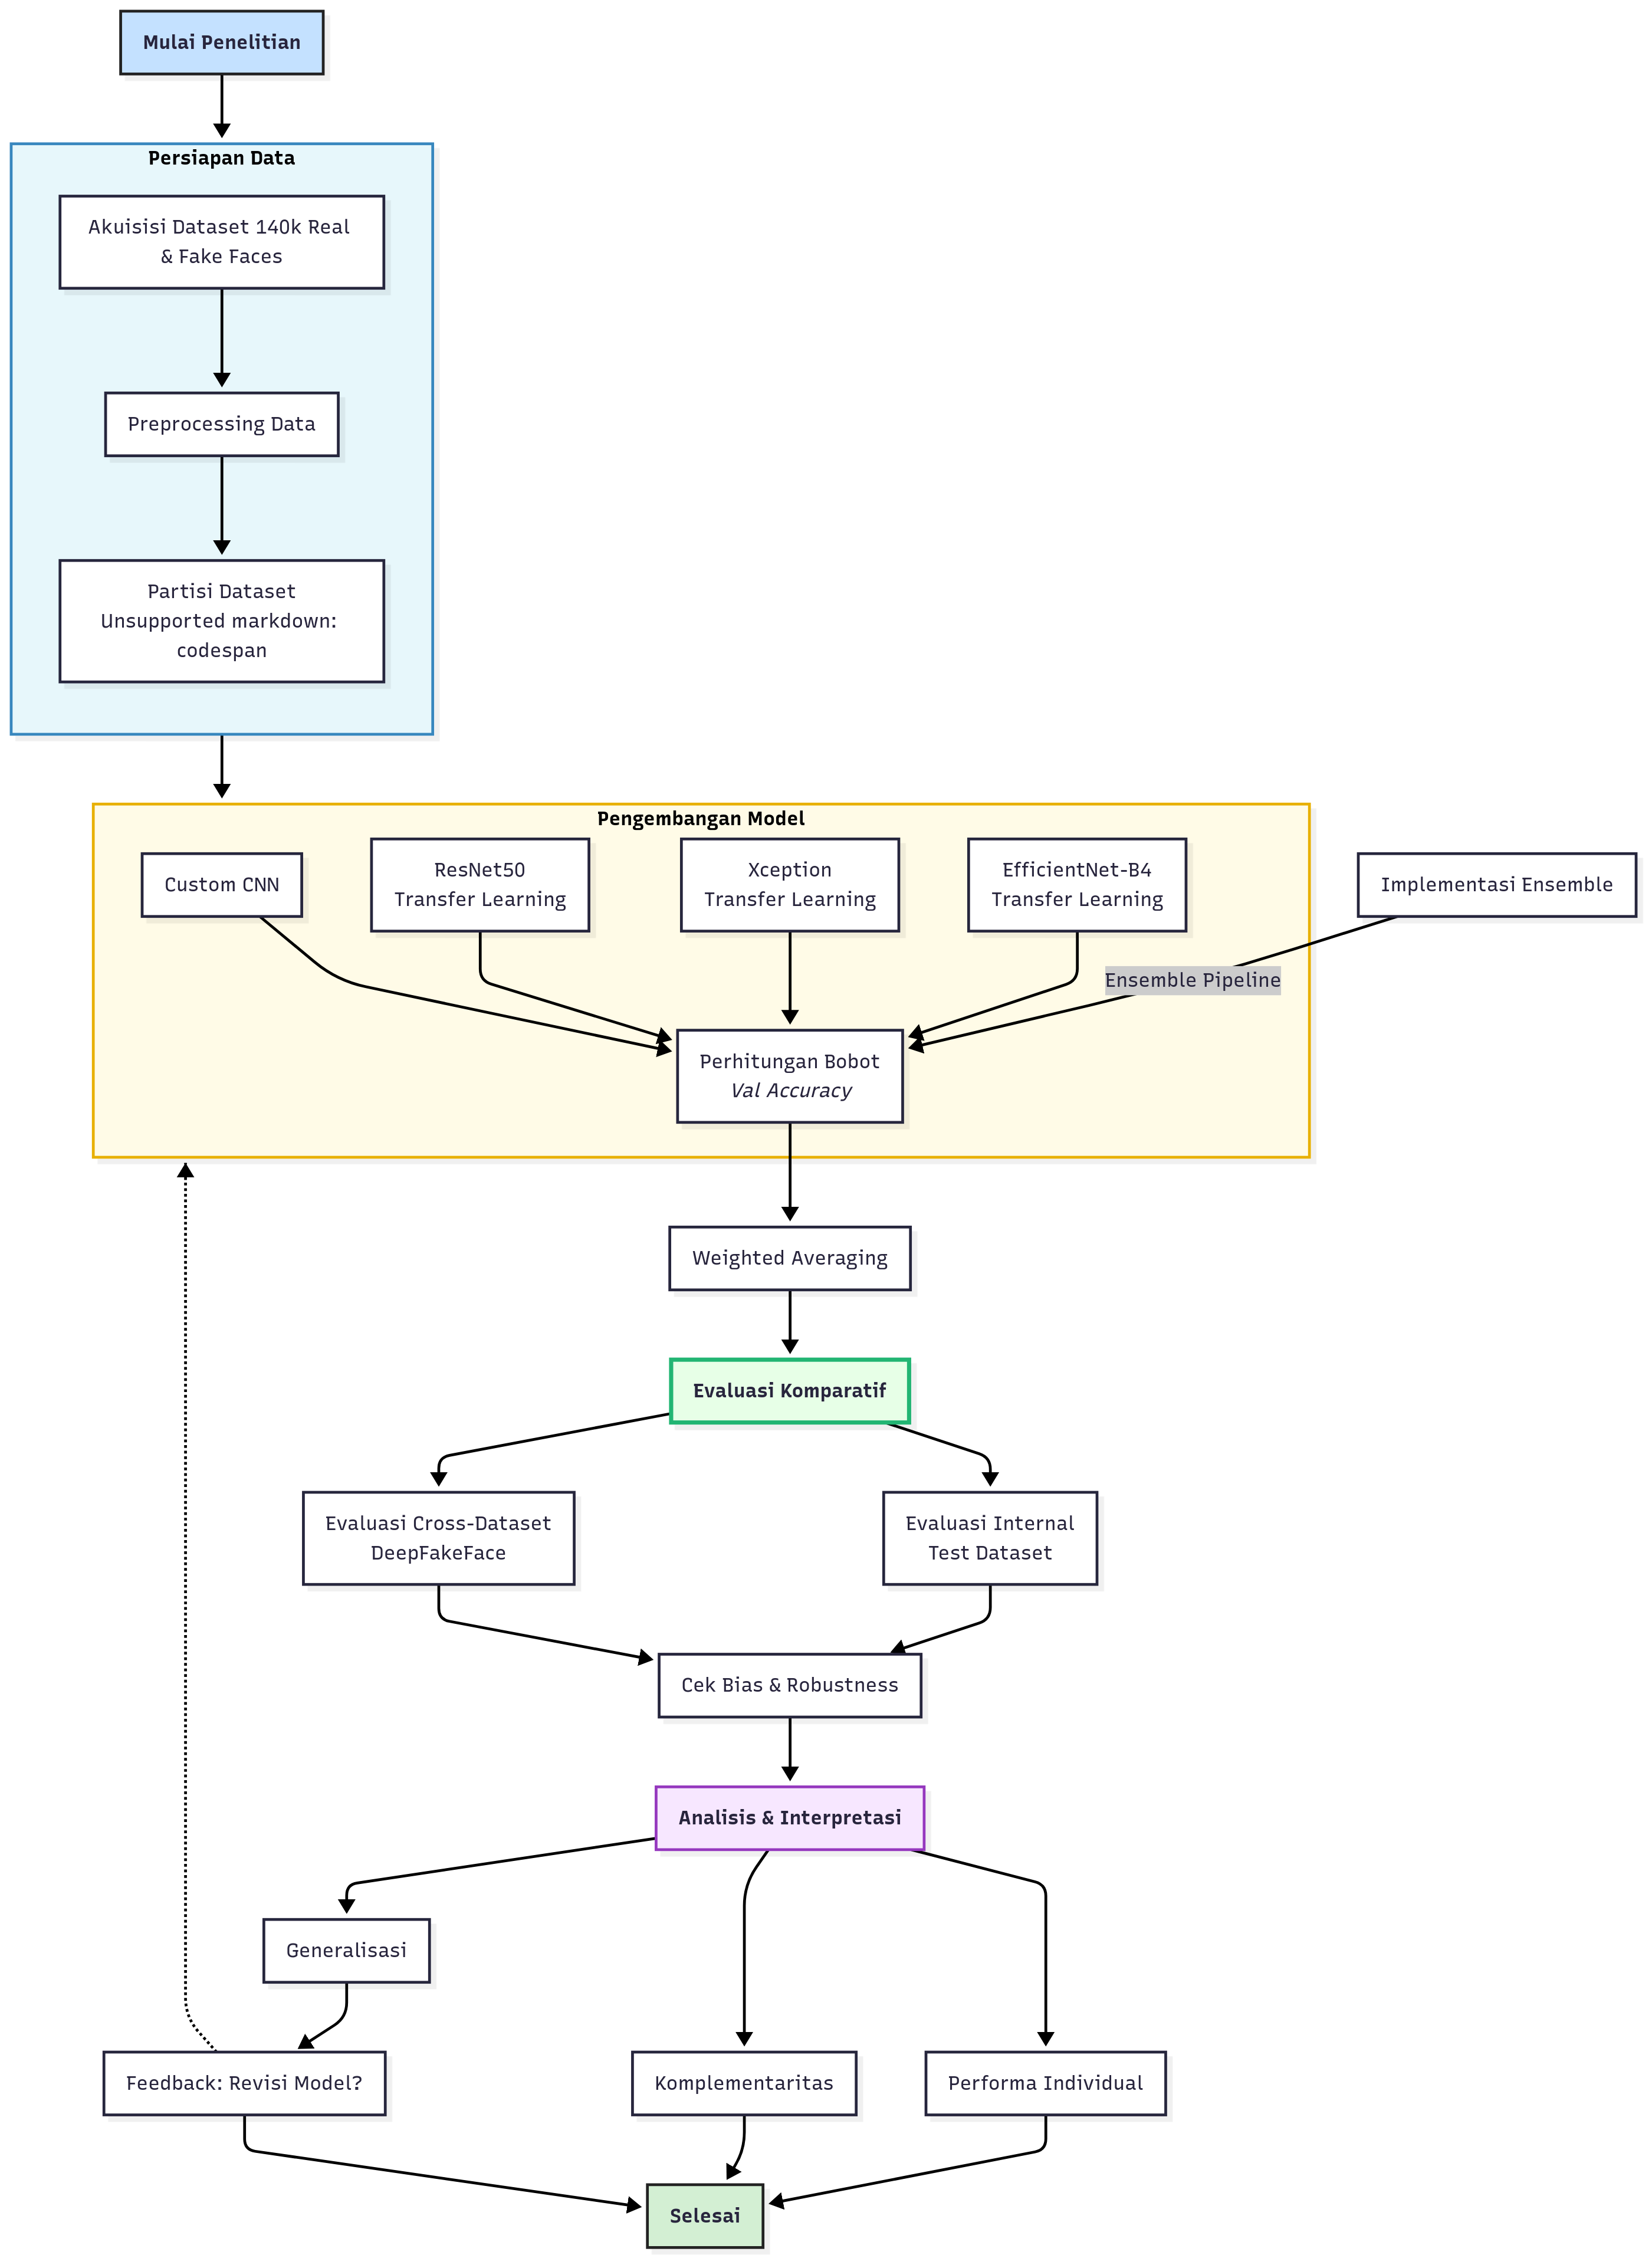
\includegraphics[width=0.85\textwidth]{assets/pics/alur-besar.png}}
    \caption{Pipeline penelitian deepfake}
    \label{fig:research_methodology}
\end{figure}

Seperti yang terlihat pada Gambar~\ref{fig:research_methodology}, metodologi penelitian mengikuti alur sistematis yang dimulai dengan persiapan data, dilanjutkan dengan pengembangan model individual dalam empat arsitektur berbeda, penghitungan bobot ensemble berdasarkan validation accuracy, implementasi weighted averaging, dan diakhiri dengan evaluasi komprehensif melalui pengujian internal maupun cross-dataset untuk analisis komplementaritas dan performa individual.

\subsection{Kerangka Penelitian}

Untuk mencapai tujuan tersebut, metodologi penelitian disusun dalam lima tahapan utama yang berurutan, sebagaimana diuraikan di bawah ini:
\begin{enumerate}
    \item \textbf{Persiapan Data}: Meliputi akuisisi, \textit{preprocessing}, dan partisi \textit{dataset} untuk memastikan data siap digunakan dalam pelatihan dan evaluasi.
    \item \textbf{Pengembangan Model Individual}: Merancang, melatih, dan mengevaluasi empat arsitektur \textit{deep learning} yang berbeda untuk menciptakan keragaman dalam \textit{ensemble}.
    \item \textbf{Implementasi \textit{Ensemble}}: Mengembangkan model \textit{ensemble weighted averaging} dengan menghitung bobot berdasarkan performa validasi dari setiap model individual.
    \item \textbf{Evaluasi Komparatif}: Melakukan perbandingan sistematis antara performa model individual dengan model \textit{ensemble} menggunakan \textit{dataset} pengujian.
    \item \textbf{Analisis dan Interpretasi}: Menganalisis hasil secara statistik untuk menarik kesimpulan mengenai efektivitas pendekatan \textit{ensemble} dan implikasi praktisnya.
\end{enumerate}

\subsection{Desain Eksperimen}

Penelitian ini menggunakan desain eksperimen terkendali untuk mengukur pengaruh arsitektur model terhadap performa deteksi. Variabel-variabel dalam penelitian ini didefinisikan sebagai berikut:
\begin{itemize}
    \item \textbf{Variabel Bebas}: Arsitektur model yang digunakan, yaitu \textit{CNN}, \textit{ResNet50}, \textit{Xception}, dan \textit{EfficientNet-B4}.
    \item \textbf{Variabel Terikat}: Metrik performa yang diukur, meliputi \textit{Accuracy}, \textit{Precision}, \textit{Recall}, \textit{F1-Score}.
    \item \textbf{Variabel Terkendali}: Faktor-faktor yang dijaga konstan untuk memastikan validitas perbandingan, seperti \textit{dataset}, pipa \textit{preprocessing}, parameter pelatihan utama, dan metodologi evaluasi.
\end{itemize}

Validitas internal dijaga melalui prosedur standarisasi yang ketat pada seluruh tahapan eksperimen. Sementara itu, validitas eksternal ditingkatkan dengan menggunakan \textit{dataset} publik yang representatif dan metodologi yang dapat direplikasi.

%-----------------------------------------------------------------------------%
\section{Dataset dan Preprocessing}
%-----------------------------------------------------------------------------%

Pemilihan dan persiapan \textit{dataset} merupakan fondasi krusial dalam penelitian ini. Tahapan ini bertujuan untuk menyediakan data yang berkualitas, seimbang, dan relevan untuk melatih serta mengevaluasi model deteksi \textit{deepfake}.

\subsection{Karakteristik Dataset}

Penelitian ini menggunakan \textit{dataset} "140k Real and Fake Faces" yang diperoleh dari repositori \textit{Kaggle}. \textit{Dataset} ini dipilih karena relevansinya dengan tugas deteksi wajah asli versus palsu dan skalanya yang besar. Karakteristik utama dari \textit{dataset} ini dirangkum dalam Tabel \ref{tab:dataset_characteristics}.

\begin{table}[H]
\centering
\caption{Karakteristik data "140k Real and Fake Faces"}
\label{tab:dataset_characteristics}
\begin{tabular}{|l|l|}
\hline
\textbf{Karakteristik} & \textbf{Spesifikasi} \\
\hline
Total Gambar & 140.000 \\
Gambar Asli (\textit{Real}) & 70.000 (50\%) \\
Gambar Palsu (\textit{Fake}) & 70.000 (50\%) \\
Format Gambar & JPEG \\
Resolusi & 256 × 256 piksel \\
\textit{Color Space} & RGB \\
Sumber Gambar Asli & \textit{Flickr} (Koleksi \textit{Nvidia}) \\
Sumber Gambar Palsu & \textit{StyleGAN Generated} \\
\hline
\end{tabular}
\end{table}

\subsection{Partisi Dataset}

Untuk memastikan evaluasi yang objektif, \textit{dataset} dibagi menjadi tiga subset: pelatihan, validasi, dan pengujian. Pembagian ini menggunakan teknik \textit{stratified sampling} untuk menjaga distribusi kelas yang seimbang pada setiap subset. Proporsi pembagiannya adalah sebagai berikut:

\begin{align}
D_{train} &= 100.000 \text{ gambar (71.4\%)} \\
D_{val} &= 20.000 \text{ gambar (14.3\%)} \\
D_{test} &= 20.000 \text{ gambar (14.3\%)}
\end{align}

\subsection{Pipa Preprocessing}

Pipa \textit{preprocessing} diimplementasikan menggunakan generator data dari framework deep learning. Proses ini mencakup normalisasi nilai piksel dan augmentasi data. Konfigurasi yang berbeda diterapkan untuk data pelatihan dan data evaluasi (validasi dan pengujian).

\subsubsection{Preprocessing Data Pelatihan}

Generator data pelatihan dikonfigurasi dengan berbagai parameter untuk mengoptimalkan proses pembelajaran. Pertama, dilakukan normalisasi piksel dengan membagi setiap nilai piksel dengan 255 untuk mengubah skala dari rentang 0-255 menjadi 0-1, yang membantu stabilitas proses pelatihan. Augmentasi data berupa \textit{horizontal flip} diterapkan secara acak pada gambar untuk meningkatkan variasi data dan mencegah overfitting. Ukuran target gambar ditetapkan pada 256×256 piksel untuk konsistensi dengan arsitektur model. Batch size diatur pada 32 untuk keseimbangan antara efisiensi komputasi dan penggunaan memori. Mode kelas ditetapkan sebagai binary karena ini adalah masalah klasifikasi dua kelas (real vs fake). Terakhir, shuffle diaktifkan untuk memastikan urutan data acak pada setiap epoch, yang membantu proses konvergensi model.

\subsubsection{Preprocessing Data Validasi dan Pengujian}

Untuk data validasi dan pengujian, konfigurasi generator dibuat lebih sederhana dan deterministik. Normalisasi piksel tetap diterapkan dengan cara yang sama seperti data pelatihan untuk konsistensi. Namun, tidak ada augmentasi data yang diterapkan untuk memastikan evaluasi dilakukan pada data orisinal yang tidak dimodifikasi. Ukuran target gambar tetap 256×256 piksel untuk konsistensi. Untuk data validasi, batch size diatur pada 16 untuk efisiensi proses evaluasi, sedangkan untuk data pengujian menggunakan batch size 1 untuk prediksi individual yang lebih presisi. Mode kelas tetap binary, dan shuffle dinonaktifkan untuk mempertahankan urutan data asli selama evaluasi.

\subsection{Strategi Augmentasi Data}

Strategi augmentasi data secara sengaja dibatasi hanya pada \textit{horizontal flipping} untuk \textit{set} pelatihan. Keputusan ini didasarkan pada pertimbangan berikut:
\begin{itemize}
    \item \textbf{Preservasi Artefak}: Menghindari augmentasi yang lebih agresif (seperti rotasi, \textit{zoom}, atau \textit{shear}) yang berpotensi menghilangkan atau merusak artefak kompresi halus yang sering menjadi penanda utama citra \textit{deepfake}.
    \item \textbf{Integritas Spasial}: Mempertahankan hubungan spasial fitur wajah yang penting untuk proses deteksi.
    \item \textbf{Efisiensi Komputasi}: Menjaga proses pelatihan agar tetap efisien secara komputasi.
\end{itemize}
Contoh visual dari penerapan augmentasi sederhana ini disajikan pada Gambar \ref{fig:augmentation_simple}, yang menunjukkan perbandingan gambar sebelum dan sesudah operasi \textit{horizontal flip}.

\begin{figure}[h]
\centering
% Menambahkan \fbox{} untuk membuat bingkai di sekitar gambar
\fbox{\includegraphics[width=0.8\textwidth]{assets/pics/augmentation_simple.png}}
\caption{Perbandingan gambar sebelum dan sesudah augmentasi sederhana (\textit{horizontal flip})}
\label{fig:augmentation_simple}
\end{figure}

%-----------------------------------------------------------------------------%
\section{Arsitektur Model Individual}
%-----------------------------------------------------------------------------%

Penelitian ini mengimplementasikan empat arsitektur \textit{deep learning} yang dipilih untuk memberikan keragaman pada model ansambel. Setiap model memiliki karakteristik komplementer, mulai dari arsitektur sederhana yang dirancang khusus hingga model \textit{state-of-the-art} yang memanfaatkan \textit{transfer learning}.

\subsection{Arsitektur Custom CNN}

Sebuah \textit{Convolutional Neural Network (CNN)} dirancang dengan arsitektur hierarkis yang memanfaatkan karakteristik CNN dalam ekstraksi fitur lokal-ke-global, dengan harapan dapat mendeteksi inkonsistensi yang umum pada citra \textit{deepfake}. Spesifikasi lengkap arsitektur disajikan pada Tabel \ref{tab:custom_cnn_arch}. Setiap blok konvolusi mengintegrasikan regularisasi \textit{Dropout} untuk mencegah \textit{overfitting}. Peningkatan jumlah \textit{filter} secara hierarkis (32 $\rightarrow$ 64 $\rightarrow$ 128 $\rightarrow$ 256) memungkinkan model untuk mempelajari fitur dari level rendah (tepi, tekstur) hingga level tinggi (pola wajah).

\begin{table}[H]
\centering
\caption{Arsitektur dari model CNN}
\label{tab:custom_cnn_arch}
\begin{tabular}{|l|l|l|l|}
\hline
\textbf{Jenis \textit{Layer}} & \textbf{\textit{Output Shape}} & \textbf{Konfigurasi} & \textbf{Aktivasi} \\
\hline
\textit{InputLayer} & (256, 256, 3) & - & - \\
\hline
\textit{Conv2D} & (256, 256, 32) & 32 \textit{filter}, 3×3 & \textit{ReLU} \\
\textit{Conv2D} & (256, 256, 32) & 32 \textit{filter}, 3×3 & \textit{ReLU} \\
\textit{MaxPooling2D} & (128, 128, 32) & 2×2 \textit{pool size} & - \\
\textit{Dropout} & (128, 128, 32) & \textit{rate}=0.25 & - \\
\hline
\textit{Conv2D} & (128, 128, 64) & 64 \textit{filter}, 3×3 & \textit{ReLU} \\
\textit{Conv2D} & (128, 128, 64) & 64 \textit{filter}, 3×3 & \textit{ReLU} \\
\textit{MaxPooling2D} & (64, 64, 64) & 2×2 \textit{pool size} & - \\
\textit{Dropout} & (64, 64, 64) & \textit{rate}=0.25 & - \\
\hline
\textit{Conv2D} & (64, 64, 128) & 128 \textit{filter}, 3×3 & \textit{ReLU} \\
\textit{Conv2D} & (64, 64, 128) & 128 \textit{filter}, 3×3 & \textit{ReLU} \\
\textit{MaxPooling2D} & (32, 32, 128) & 2×2 \textit{pool size} & - \\
\textit{Dropout} & (32, 32, 128) & \textit{rate}=0.25 & - \\
\hline
\textit{Conv2D} & (32, 32, 256) & 256 \textit{filter}, 3×3 & \textit{ReLU} \\
\textit{Conv2D} & (32, 32, 256) & 256 \textit{filter}, 3×3 & \textit{ReLU} \\
\textit{MaxPooling2D} & (16, 16, 256) & 2×2 \textit{pool size} & - \\
\textit{Dropout} & (16, 16, 256) & \textit{rate}=0.25 & - \\
\hline
\textit{Flatten} & (65536,) & - & - \\
\textit{Dense} & (512,) & \textit{L2 reg}=0.01 & \textit{ReLU} \\
\textit{BatchNormalization} & (512,) & - & - \\
\textit{Dropout} & (512,) & \textit{rate}=0.5 & - \\
\textit{Dense} & (128,) & \textit{L2 reg}=0.01 & \textit{ReLU} \\
\textit{BatchNormalization} & (128,) & - & - \\
\textit{Dropout} & (128,) & \textit{rate}=0.5 & - \\
\textit{Dense (Output)} & (1,) & - & \textit{Sigmoid} \\
\hline
\end{tabular}
\end{table}

\subsection{Arsitektur Transfer Learning}

Tiga model lainnya diimplementasikan menggunakan pendekatan \textit{transfer learning} dengan bobot \textit{pre-train} dari \textit{ImageNet}. Strategi \textit{fine-tuning} diterapkan pada semua model ini.

\subsubsection{ResNet50}
Model \textit{ResNet50} dipilih karena kemampuannya mengatasi masalah \textit{vanishing gradient} melalui \textit{residual connection}. Strategi \textit{fine-tuning} diterapkan dengan membekukan 100 \textit{layer} pertama untuk mempertahankan fitur umum tingkat rendah, sementara \textit{layer}-*\textit{layer}* berikutnya dilatih ulang untuk beradaptasi dengan domain deteksi \textit{deepfake}.

\subsubsection{Xception}
Arsitektur \textit{Xception} (Extreme Inception) memanfaatkan \textit{depthwise separable convolutions} untuk ekstraksi fitur yang efisien. Operasi ini memisahkan korelasi spasial dan \textit{cross-channel}, menjadikannya sangat efektif dalam menangkap inkonsistensi halus pada citra yang dimanipulasi secara digital seperti \textit{deepfake}.

\subsubsection{EfficientNet-B4}
\textit{EfficientNet-B4} dipilih karena pendekatan \textit{compound scaling} yang inovatif, yang secara seimbang menskalakan kedalaman (\textit{depth}), lebar (\textit{width}), dan resolusi jaringan. Hal ini menghasilkan keseimbangan optimal antara akurasi dan efisiensi komputasi, menjadikannya kandidat yang kuat untuk aplikasi praktis.

%-----------------------------------------------------------------------------%
\section{Metodologi Ensemble Weighted Averaging}
%-----------------------------------------------------------------------------%

Untuk meningkatkan robustisitas dan akurasi deteksi, prediksi dari keempat model individual digabungkan menggunakan metode \textit{ensemble weighted averaging}. Bagian ini menjelaskan dasar teoretis, strategi penentuan bobot, implementasi teknis, dan contoh perhitungan konkret dari pendekatan ini.

\subsection{Fondasi Teoretis}

\textit{Ensemble weighted averaging} beroperasi pada prinsip bahwa kombinasi linear dari beberapa model yang beragam, dengan bobot yang ditetapkan secara strategis, dapat menghasilkan prediksi yang lebih akurat dan stabil daripada prediksi model tunggal mana pun. Berdasarkan formulasi matematika yang telah dijelaskan dalam Bab 2 (Persamaan~\ref{eq:weighted_ensemble}).

\subsection{Strategi Perhitungan Bobot}

Bobot ($w_i$) untuk setiap model tidak ditetapkan secara seragam, melainkan dihitung berdasarkan performa masing-masing model pada \textit{dataset} validasi menggunakan formula yang telah didefinisikan dalam Persamaan~\ref{eq:performance_weight}. Pendekatan ini secara intuitif memberikan pengaruh yang lebih besar kepada model dengan performa validasi terbaik, sambil tetap mempertimbangkan kontribusi dari model lainnya.

\subsection{Contoh Perhitungan Bobot Ensemble}

Untuk memberikan pemahaman yang lebih konkret mengenai mekanisme perhitungan bobot, berikut disajikan contoh perhitungan menggunakan data hipotetis yang mudah dipahami:

\subsubsection{Skenario Contoh}
Misalkan kita memiliki empat model dengan validation accuracy sebagai berikut:
\begin{itemize}
    \item Model A (Custom CNN): 95,0\%
    \item Model B (ResNet50): 88,0\%
    \item Model C (Xception): 97,0\%
    \item Model D (EfficientNet): 92,0\%
\end{itemize}

\subsubsection{Langkah 1: Menghitung Total Validation Accuracy}
$$\text{Total} = 95,0 + 88,0 + 97,0 + 92,0 = 372,0$$

\subsubsection{Langkah 2: Menghitung Bobot Individual}
Menggunakan Persamaan~\ref{eq:performance_weight}:

\begin{align}
w_A &= \frac{95,0}{372,0} = 0,255 \text{ (25,5\%)} \\
w_B &= \frac{88,0}{372,0} = 0,237 \text{ (23,7\%)} \\
w_C &= \frac{97,0}{372,0} = 0,261 \text{ (26,1\%)} \\
w_D &= \frac{92,0}{372,0} = 0,247 \text{ (24,7\%)}
\end{align}

\subsubsection{Langkah 3: Verifikasi}
$$w_A + w_B + w_C + w_D = 0,255 + 0,237 + 0,261 + 0,247 = 1,000 \checkmark$$

\subsection{Mekanisme Prediksi Ensemble}

Setelah bobot diperoleh, prediksi ensemble untuk sebuah input $x$ dihitung sebagai berikut:

\subsubsection{Skenario Prediksi}
Misalkan untuk sebuah citra input, masing-masing model menghasilkan probabilitas:
\begin{itemize}
    \item Model A: 0,85 (85\% yakin citra adalah deepfake)
    \item Model B: 0,78 (78\% yakin citra adalah deepfake)
    \item Model C: 0,92 (92\% yakin citra adalah deepfake)
    \item Model D: 0,81 (81\% yakin citra adalah deepfake)
\end{itemize}

\subsubsection{Perhitungan Prediksi Ensemble}
Menggunakan Persamaan~\ref{eq:weighted_ensemble}:

\begin{align}
\hat{y}_{ensemble} &= (0,255 \times 0,85) + (0,237 \times 0,78) + (0,261 \times 0,92) + (0,247 \times 0,81) \\
&= 0,217 + 0,185 + 0,240 + 0,200 \\
&= 0,842
\end{align}

Hasil ini berarti model ensemble memiliki confidence 84,2\% bahwa citra tersebut adalah deepfake.

\subsection{Kerangka Implementasi}

Model \textit{ensemble} dibangun menggunakan API fungsional untuk menggabungkan beberapa model klasifikasi citra yang telah dilatih sebelumnya. Setiap model individual diperlakukan sebagai \textit{feature extractor} dan tidak diperbarui lagi selama proses inferensi dengan membekukan bobotnya.

Implementasi ansambel ini mengadopsi pendekatan \textit{weighted averaging}, di mana proses dimulai dengan pembuatan layer input yang konsisten untuk semua model dengan bentuk (256, 256, 3). Setiap model yang telah dilatih kemudian menerima input yang sama dan menghasilkan output probabilistik individual. Output dari masing-masing model kemudian dikalikan dengan bobot yang telah dihitung berdasarkan performa validasi mereka. Bobot ini mencerminkan kontribusi relatif setiap model terhadap prediksi akhir, dimana model dengan akurasi validasi yang lebih tinggi mendapat bobot yang lebih besar. Hasil perkalian antara output model dan bobotnya kemudian dijumlahkan untuk menghasilkan prediksi ensemble final. Seluruh proses ini diintegrasikan dalam satu model ensemble yang dapat melakukan inferensi secara end-to-end, mengambil input citra dan menghasilkan prediksi gabungan yang memanfaatkan kekuatan kolektif dari semua model individual.

%-----------------------------------------------------------------------------%
\section{Prosedur Pelatihan}
%-----------------------------------------------------------------------------%

Untuk memastikan perbandingan yang objektif dan valid antara model individual dan pendekatan \textit{ensemble}, penelitian ini menerapkan serangkaian prosedur pelatihan yang terstandarisasi. Bagian ini merinci protokol pelatihan yang digunakan, termasuk konfigurasi \textit{hyperparameter} dan \textit{callback}.

\subsection{Protokol Pelatihan}

Setiap model individual dilatih menggunakan protokol yang konsisten untuk menjamin keadilan dalam perbandingan. Perbedaan hanya terdapat pada \textit{learning rate} awal, yang disesuaikan berdasarkan karakteristik arsitektur (\textit{custom} vs. \textit{transfer learning}).

\subsubsection{Konfigurasi \textit{Hyperparameter}}
\textit{Hyperparameter} yang digunakan selama fase pelatihan dirangkum dalam Tabel \ref{tab:hyperparameters}.

\begin{table}[h]
\centering
\caption{\textit{Hyperparameter} yang digunakan untuk pelatihan model}
\label{tab:hyperparameters}
\begin{tabular}{|l|l|l|}
\hline
\textbf{Parameter} & \textbf{\textit{Custom CNN}} & \textbf{Model \textit{Transfer Learning}} \\
\hline
\textit{Optimizer} & \textit{Adam} & \textit{Adam} \\
\textit{Learning Rate} & $1 \times 10^{-4}$ & $5 \times 10^{-5}$ \\
Fungsi \textit{Loss} & \textit{Binary Crossentropy} & \textit{Binary Crossentropy} \\
\textit{Batch Size} (Latih) & 32 & 32 \\
\textit{Batch Size} (Val) & 16 & 16 \\
\textit{Max Epochs} & 15 & 15 \\
\textit{Early Stopping Patience} & 3 & 3 \\
\hline
\end{tabular}
\end{table}

\textit{Hyperparameter} dipilih berdasarkan best practices dan eksperimen awal:

\begin{itemize}
    \item Learning Rate: Model custom menggunakan $1 \times 10^{-4}$ (lebih tinggi karena training from scratch), sedangkan transfer learning menggunakan $5 \times 10^{-5}$ (lebih rendah untuk fine-tuning)   
    \item \textit{Adam Optimizer}: Dipilih karena \textit{adaptive learning rate} dan \textit{momentum}
    \item \textit{Binary Crossentropy}: Sesuai untuk klasifikasi biner 
    \item Batch Size: 32 untuk \textit{training} memberikan keseimbangan antara stabilitas dan efisiensi memori
    \item \textit{Early Stopping Patience 3}: Mencegah \textit{overfitting} dengan menghentikan \textit{training} jika tidak ada peningkatan selama 3 \textit{epoch} berturut-turut
\end{itemize}

\subsubsection{Konfigurasi callback pada model pelatihan}

Untuk mengelola proses pelatihan secara otomatis, serangkaian \textit{callback} diimplementasikan untuk mengoptimalkan hasil pelatihan. Konfigurasi \textit{callback} memiliki dua komponen utama yang bekerja secara sinergis.

Komponen pertama adalah \textit{EarlyStopping} yang berfungsi sebagai mekanisme pengawasan otomatis terhadap proses pelatihan. Callback ini secara kontinyu memonitor \textit{validation loss} pada setiap epoch dan akan menghentikan proses pelatihan secara otomatis jika tidak ada perbaikan yang signifikan selama 3 epoch berturut-turut. Parameter \textit{patience} diatur pada nilai 3 untuk memberikan toleransi yang wajar terhadap fluktuasi minor dalam performa validasi. Fitur \textit{restore best weights} diaktifkan untuk memastikan bahwa ketika pelatihan dihentikan, model akan dikembalikan ke bobot terbaik yang pernah dicapai selama proses pelatihan, bukan bobot dari epoch terakhir yang mungkin sudah mengalami overfitting.

Komponen kedua adalah \textit{ModelCheckpoint} yang berperan sebagai sistem penyimpanan otomatis untuk model terbaik. Callback ini secara terus-menerus memantau \textit{validation loss} dan secara otomatis menyimpan snapshot model setiap kali ditemukan performa yang lebih baik. File model disimpan dengan nama yang mencakup identifikasi model spesifik untuk memudahkan identifikasi. Parameter \textit{save best only} diaktifkan untuk memastikan hanya model dengan performa terbaik yang disimpan, menghemat ruang penyimpanan dan memudahkan proses evaluasi selanjutnya. Mode monitoring diatur pada 'min' karena tujuannya adalah meminimalkan validation loss.

%-----------------------------------------------------------------------------%
\section{Lingkungan Komputasi dan Reprodusibilitas}
%-----------------------------------------------------------------------------%

Bagian ini merinci spesifikasi perangkat keras dan lunak yang digunakan dalam eksperimen untuk memastikan transparansi dan memfasilitasi reprodusibilitas hasil penelitian.

\subsection{Spesifikasi Perangkat Keras dan Lunak}

Eksperimen dilakukan pada platform \textit{cloud computing} untuk memanfaatkan akselerasi GPU. Konfigurasi utama lingkungan komputasi disajikan pada Tabel \ref{tab:hardware_spec} dan \ref{tab:software_deps}.

\begin{table}[h]
\centering
\caption{Konfigurasi perangkat keras}
\label{tab:hardware_spec}
\begin{tabular}{|l|l|}
\hline
\textbf{Komponen} & \textbf{Spesifikasi} \\
\hline
Platform & \textit{Google Colaboratory Pro+} \\
GPU & \textit{NVIDIA A100 / V100} \\
Memori GPU & $\geq$ 16 GB GDDR6 \\
RAM Sistem & $\geq$ 16 GB \\
Penyimpanan & \textit{Google Drive Cloud Storage} \\
\hline
\end{tabular}
\end{table}

\begin{table}[h]
\centering
\caption{Dependensi utama yang digunakan untuk pengembangan model \textit{machine learning}}
\label{tab:software_deps}
\begin{tabular}{|l|l|}
\hline
\textbf{\textit{Framework}/Pustaka} & \textbf{Versi} \\
\hline
\textit{Python} & 3.9+ \\
\textit{TensorFlow} & 2.12+ \\
\textit{Keras} & 2.12+ \\
\textit{NumPy} & 1.23+ \\
\textit{Pandas} & 1.5+ \\
\textit{Scikit-learn} & 1.2+ \\
\textit{Matplotlib} & 3.7+ \\
\hline
\end{tabular}
\end{table}

\subsection{Langkah Reprodusibilitas}

Untuk menjamin bahwa hasil eksperimen dapat direplikasi, beberapa langkah penting diterapkan dalam proses implementasi. Reprodusibilitas menjadi aspek krusial dalam eksperimen berbasis pembelajaran mesin, mengingat banyak proses di dalamnya bersifat stokastik, seperti inisialisasi bobot, pemilihan batch, dan augmentasi data.

Langkah paling mendasar adalah dengan menetapkan \textit{random seed} secara konsisten pada semua pustaka yang digunakan. Pustaka seperti Python random, NumPy, dan TensorFlow memiliki sumber acak masing-masing yang perlu dikendalikan agar eksperimen dapat menghasilkan hasil yang konsisten setiap kali dijalankan. Proses inisialisasi reprodusibilitas dimulai dengan pengaturan seed untuk modul random Python standar, dilanjutkan dengan konfigurasi seed untuk NumPy yang mengendalikan operasi matematis acak, dan kemudian pengaturan seed untuk TensorFlow yang mengatur randomness dalam operasi deep learning. Selain itu, variabel lingkungan PYTHONHASHSEED juga diatur untuk menghindari variasi akibat proses hashing internal Python. Semua pengaturan ini dilakukan dengan menggunakan nilai seed yang tetap, yaitu 42, untuk memastikan konsistensi across different runs.

%-----------------------------------------------------------------------------%
\chapter{\babEmpat}
%-----------------------------------------------------------------------------%

Bab ini menyajikan hasil eksperimen dari implementasi sistem deteksi \textit{deepfake} menggunakan \textit{ensemble weighted averaging} yang menggabungkan empat arsitektur \textit{deep learning}. Hasil yang disajikan meliputi analisis performa model individual, implementasi sistem \textit{ensemble}, evaluasi komparatif, dan diskusi komprehensif terhadap \textit{findings} yang diperoleh.

%-----------------------------------------------------------------------------%
\section{Overview Pipeline Eksperimen}
%-----------------------------------------------------------------------------%

Sebelum menyajikan hasil detail, penting untuk memahami keseluruhan pipeline implementasi yang telah dilakukan. Gambar~\ref{fig:implementation_pipeline} mengilustrasikan tahapan lengkap eksperimen, mulai dari pre-processing hingga post-processing, yang menjadi dasar bagi semua hasil yang akan dibahas dalam bab ini.

\begin{figure}[H]
    \centering
    \fbox{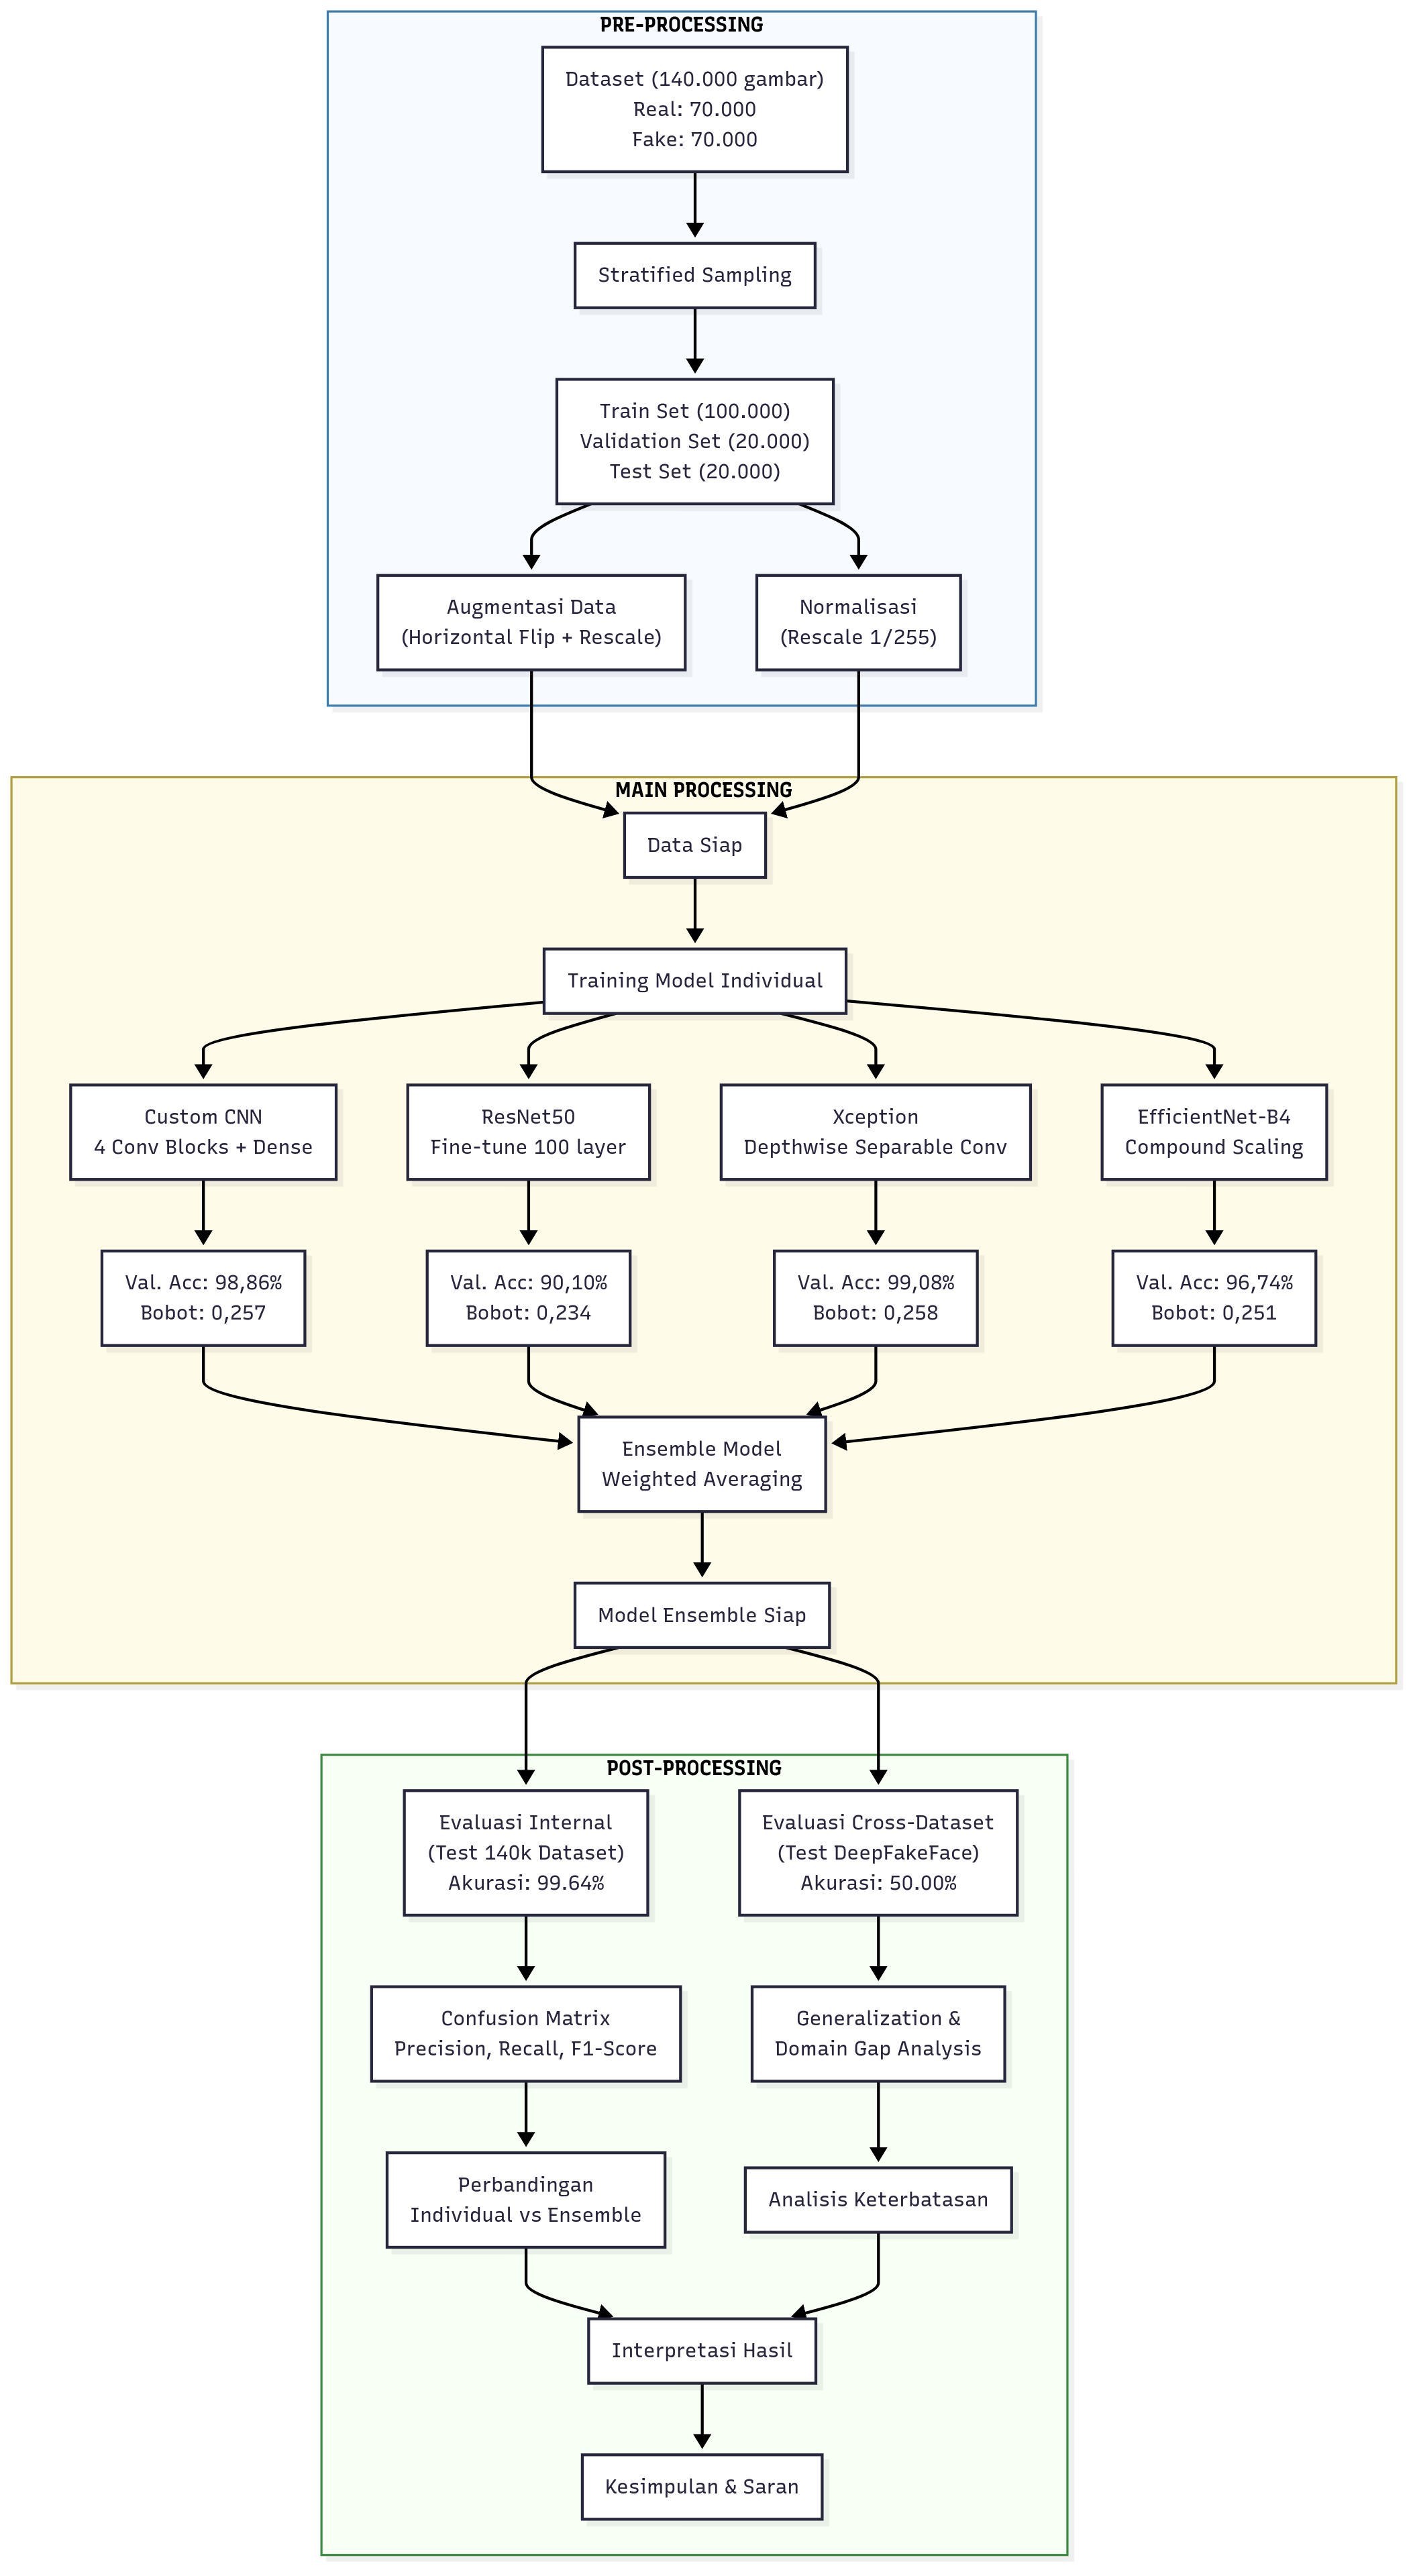
\includegraphics[width=0.85\textwidth]{assets/pics/pro-main-post.png}}
    \caption{Pipeline implementasi lengkap: pre-processing, main processing, dan post-processing}
    \label{fig:implementation_pipeline}
\end{figure}

Pipeline eksperimen ini terdiri dari tiga tahapan utama yang saling berkesinambungan:

\begin{enumerate}
    \item \textbf{Pre-processing (Tahap Biru)}: Meliputi akuisisi dataset "140k Real and Fake Faces" dengan komposisi seimbang 70.000 gambar asli dan 70.000 gambar palsu, stratified sampling untuk pembagian train/validation/test set, serta aplikasi augmentasi data minimal (horizontal flip) dan normalisasi (rescale 1/255) untuk mempertahankan artefak deteksi \textit{deepfake}.

    \item \textbf{Main Processing (Tahap Kuning)}: Merupakan inti eksperimen yang mencakup pelatihan empat model individual secara parallel (Custom CNN, ResNet50, Xception, EfficientNet-B4), penghitungan bobot ensemble berdasarkan validation accuracy menggunakan Persamaan~\ref{eq:performance_weight}, dan implementasi \textit{ensemble weighted averaging} sesuai Persamaan~\ref{eq:weighted_ensemble}.

    \item \textbf{Post-processing (Tahap Hijau)}: Evaluasi komprehensif melalui pengujian internal pada test set (akurasi 99,64\%), evaluasi cross-dataset menggunakan dataset eksternal DeepFakeFace (akurasi 50,0\%), analisis confusion matrix untuk memahami karakteristik kesalahan, perbandingan performa individual vs ensemble, dan interpretasi hasil untuk menjawab research questions.
\end{enumerate}

Setiap tahap dirancang dengan tujuan spesifik untuk menjawab research questions yang telah diformulasikan, dengan emphasis khusus pada komplementaritas model dalam tahap ensemble averaging. Hasil dari pipeline ini menunjukkan peningkatan performa yang konsisten dari model individual terbaik (Xception: 99,20\%) ke ensemble (99,64\%), dengan reduksi signifikan dalam false negatives dan false positives.

%-----------------------------------------------------------------------------%
\section{Hasil Pelatihan Model Individual}
%-----------------------------------------------------------------------------%
Tahap pertama dalam analisis adalah mengevaluasi performa dari masing-masing dari empat arsitektur yang dilatih secara individual. Bagian ini akan merinci hasil pelatihan, kurva pembelajaran, serta metrik evaluasi akhir pada \textit{dataset} pengujian untuk model \textit{Custom CNN}, \textit{ResNet50}, \textit{Xception}, dan \textit{EfficientNet-B4}. Hasil-hasil ini menjadi fondasi untuk pembobotan dan evaluasi sistem \textit{ensemble}.


\subsection{Performa Model CNN}

Model CNN yang dirancang khusus untuk deteksi \textit{deepfake} menunjukkan pembelajaran yang stabil tanpa menunjukkan hasil yang overfitting. Model mencapai konvergensi pada \textit{epoch} ke-12 dengan \textit{validation accuracy} tertinggi 98,86\%.

\begin{figure}[H]
    \centering
    \fbox{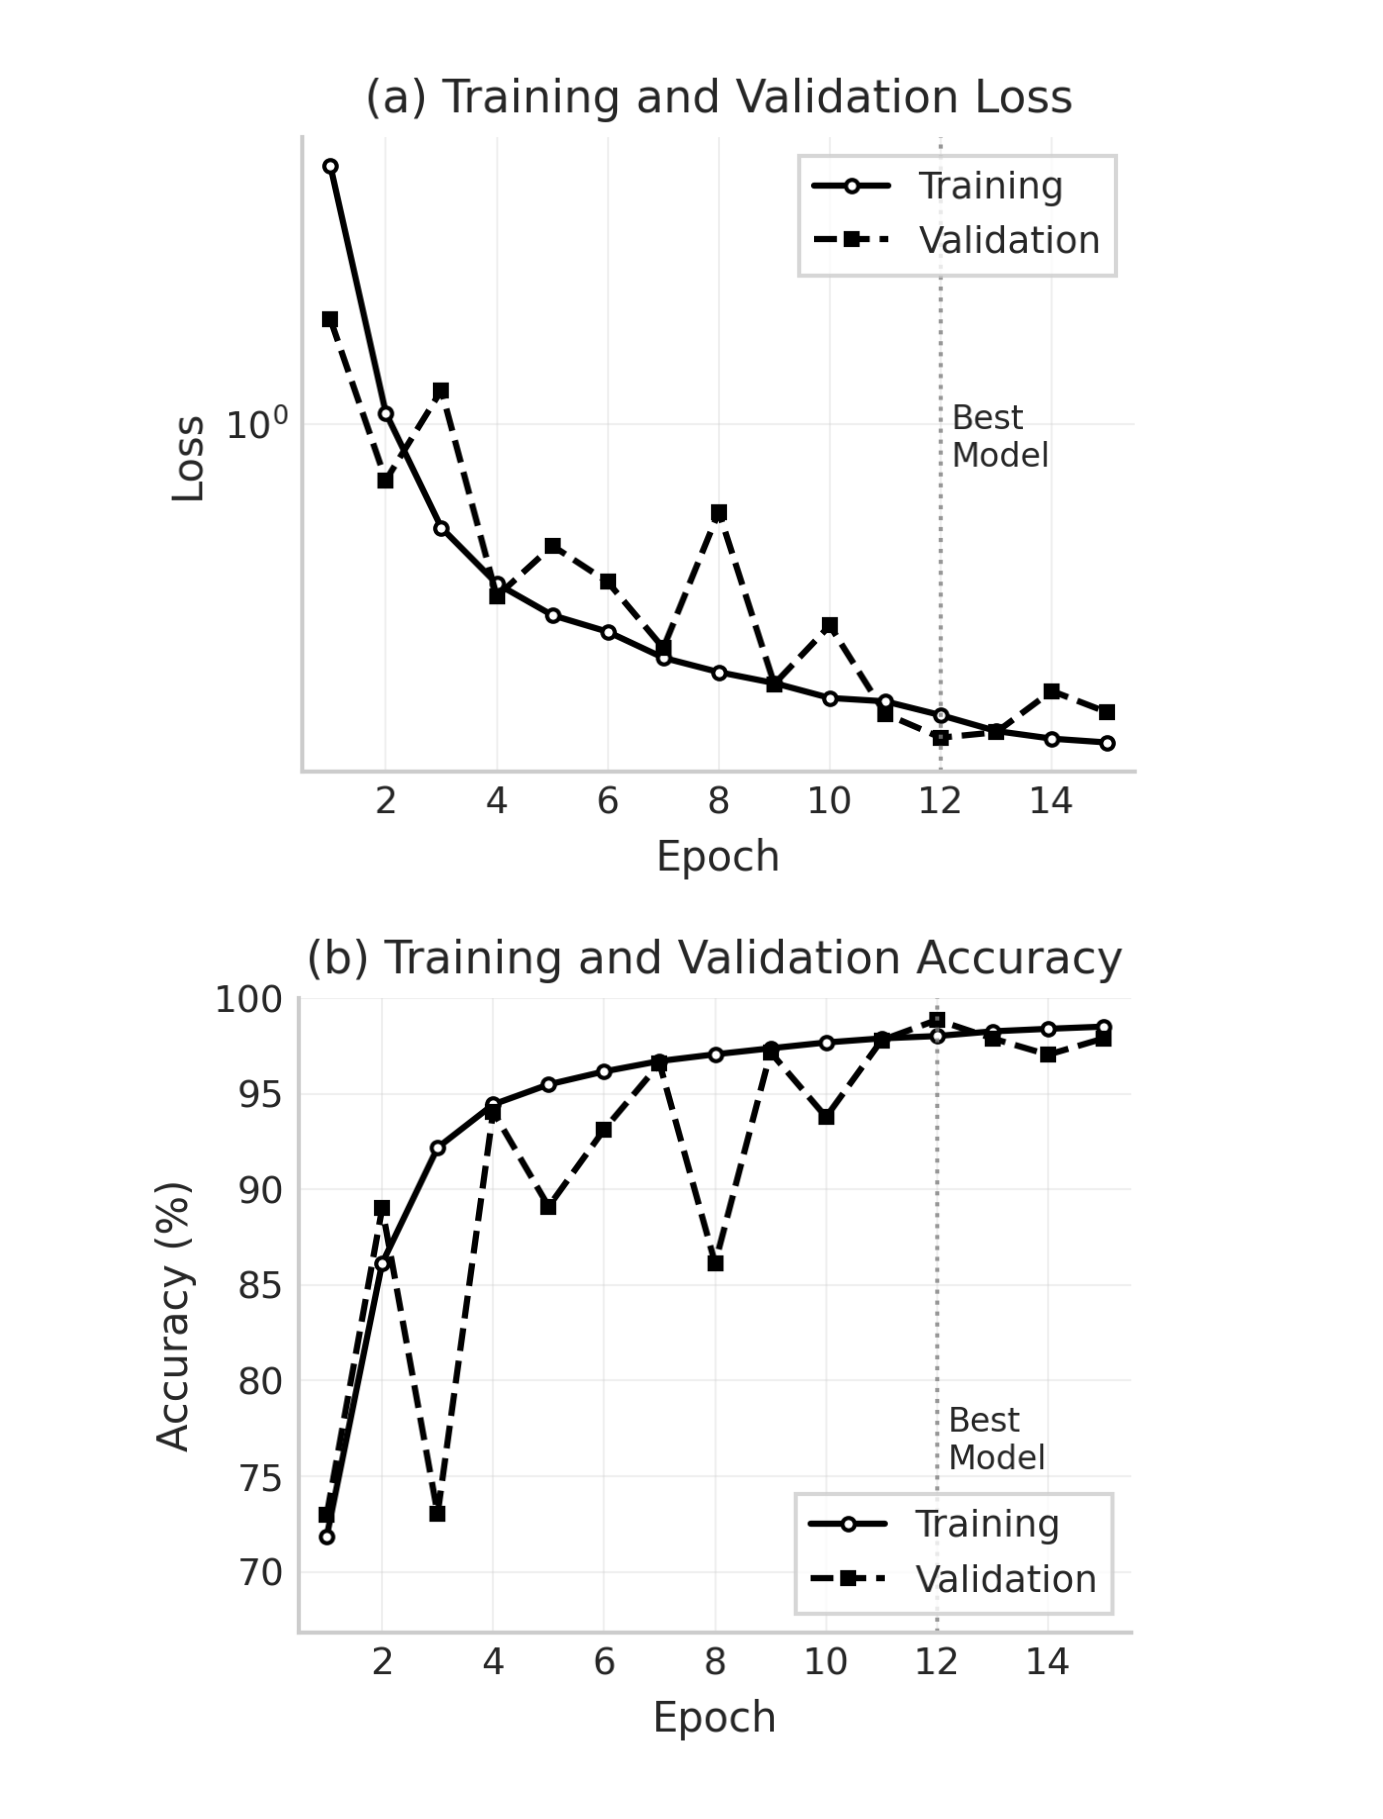
\includegraphics[width=0.6\textwidth]{assets/pics/cnn_training_curves (1).png}}
    \caption{Kurva pelatihan model \textit{CNN} menunjukkan \textit{loss} dan akurasi selama proses pembelajaran}
    \label{fig:cnn_training}
\end{figure}


Analisis kurva pelatihan pada Gambar~\ref{fig:cnn_training} menunjukkan bahwa model \textit{Custom CNN} mengalami pembelajaran yang konsisten dengan beberapa fluktuasi pada \textit{validation accuracy}, namun secara keseluruhan menunjukkan tren peningkatan yang baik.

\begin{table}[H]
\centering
\caption{Metrik evaluasi dari model CNN}
\label{tab:cnn_results}
\begin{tabular}{|l|c|}
\hline
\textbf{Metrik} & \textbf{Nilai} \\
\hline
\textit{Best Validation Accuracy} & 98,86\% \\
\textit{Test Accuracy} & 98,81\% \\
\textit{Test Precision} & 99,02\% \\
\textit{Test Recall} & 98,60\% \\
\textit{Test F1-Score} & 98,81\% \\
\hline
\end{tabular}
\end{table}

\subsection{Performa Model ResNet50}

Model \textit{ResNet50} dengan \textit{transfer learning} menunjukkan performa yang lebih rendah dari yang diharapkan. Meskipun menggunakan \textit{pre-trained weights} dari \textit{ImageNet}, model ini mengalami kesulitan dalam konvergensi dan menunjukkan tanda-tanda \textit{overfitting}.

\begin{figure}[H]
    \centering
    \fbox{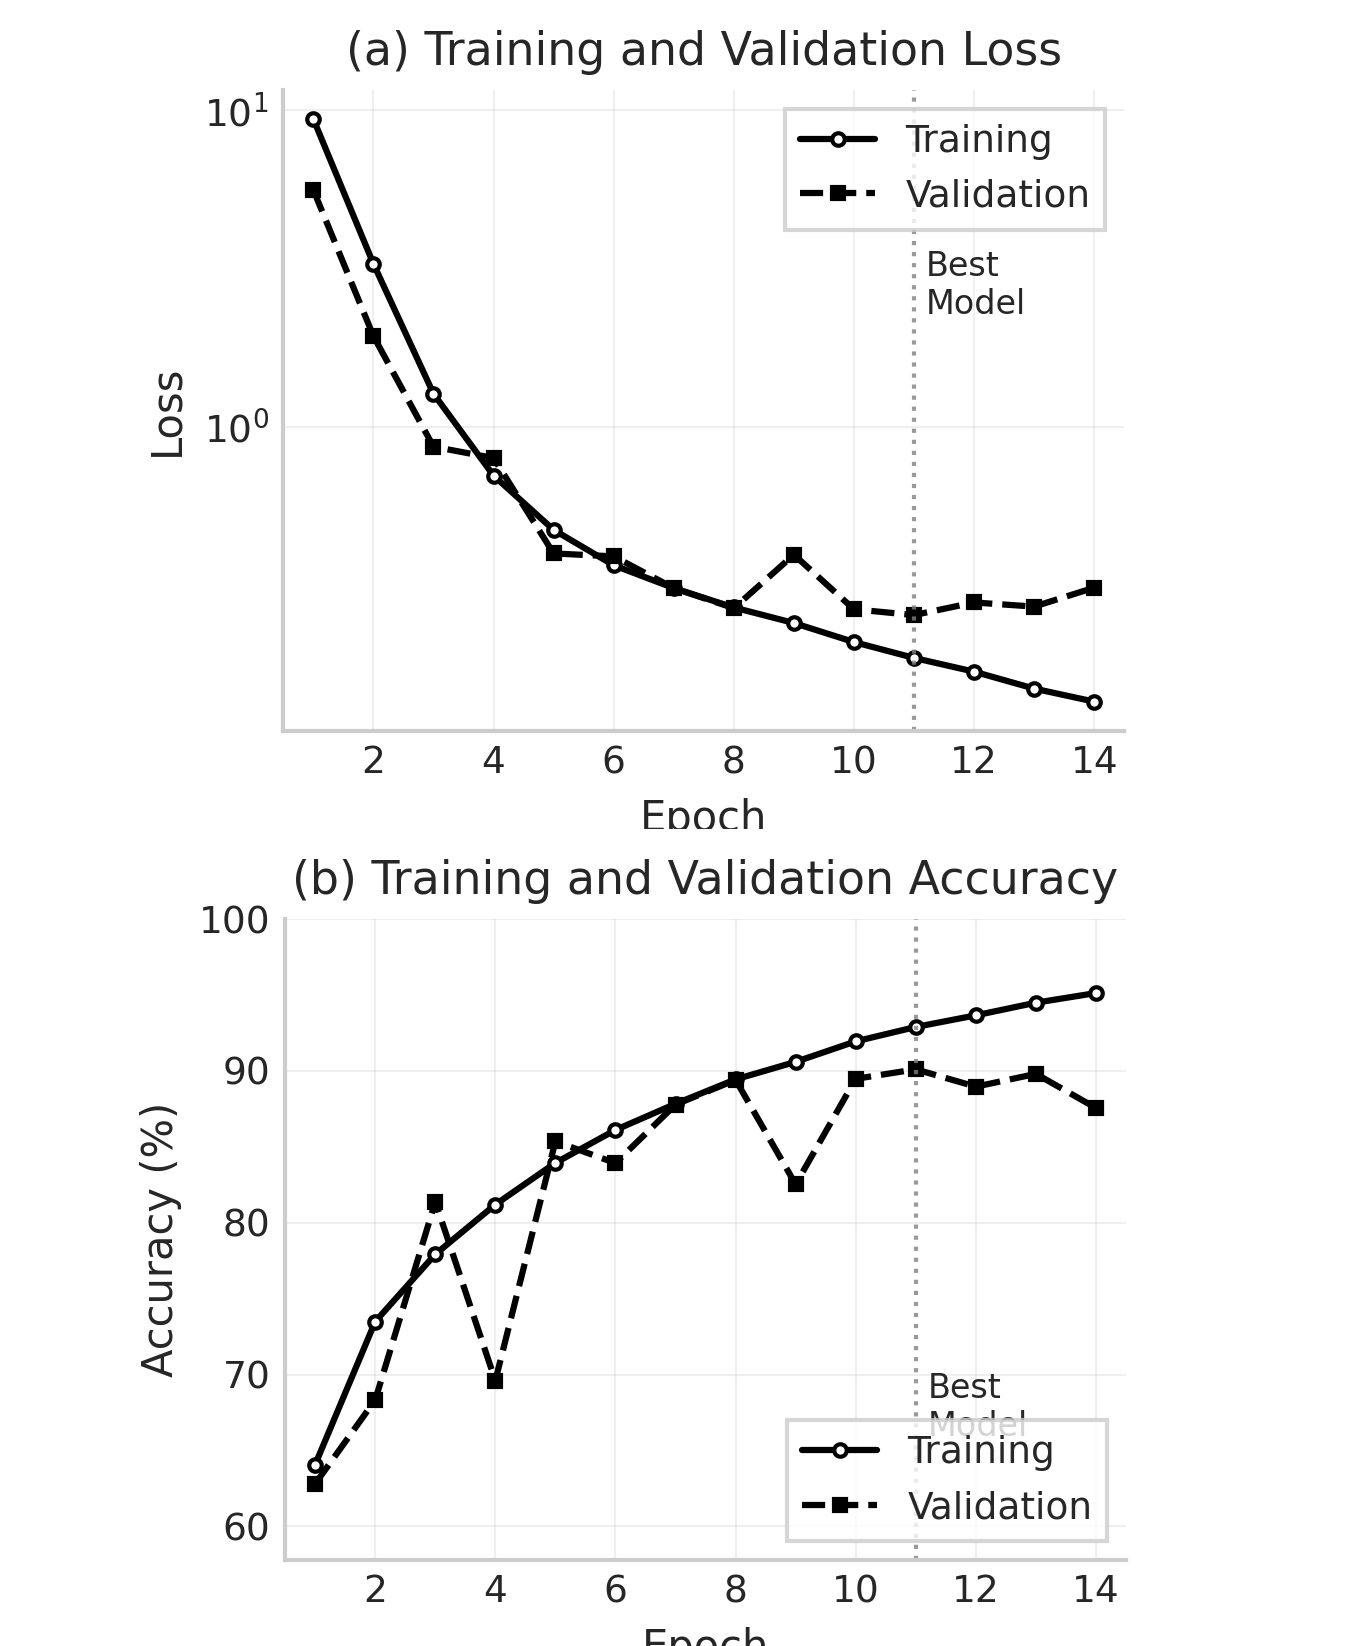
\includegraphics[width=0.6\textwidth]{assets/pics/resnet_training_curves (1).png}}
    \caption{Kurva pelatihan model \textit{ResNet50} dengan strategi \textit{transfer learning}}
    \label{fig:resnet_training}
\end{figure}

Kurva pelatihan pada Gambar~\ref{fig:resnet_training} menunjukkan fluktuasi yang signifikan pada \textit{validation accuracy} dan mencapai performa terbaik pada \textit{epoch} ke-11.

\begin{table}[H]
\centering
\caption{Metrik evaluasi dari model \textit{ResNet50}}
\label{tab:resnet_results}
\begin{tabular}{|l|c|}
\hline
\textbf{Metrik} & \textbf{Nilai} \\
\hline
\textit{Best Validation Accuracy} & 90,10\% \\
\textit{Test Accuracy} & 90,10\% \\
\textit{Test Precision} & 86,49\% \\
\textit{Test Recall} & 95,03\% \\
\textit{Test F1-Score} & 90,56\% \\
\hline
\end{tabular}
\end{table}

\subsection{Performa Model Xception}

Model \textit{Xception} dengan arsitektur \textit{depthwise separable convolution} menunjukkan performa terbaik di antara keempat model individual. Model mencapai konvergensi yang sangat baik dengan \textit{early stopping} pada \textit{epoch} ke-9 dan mempertahankan performa hingga \textit{epoch} ke-12.

\begin{figure}[H]
    \centering
    \fbox{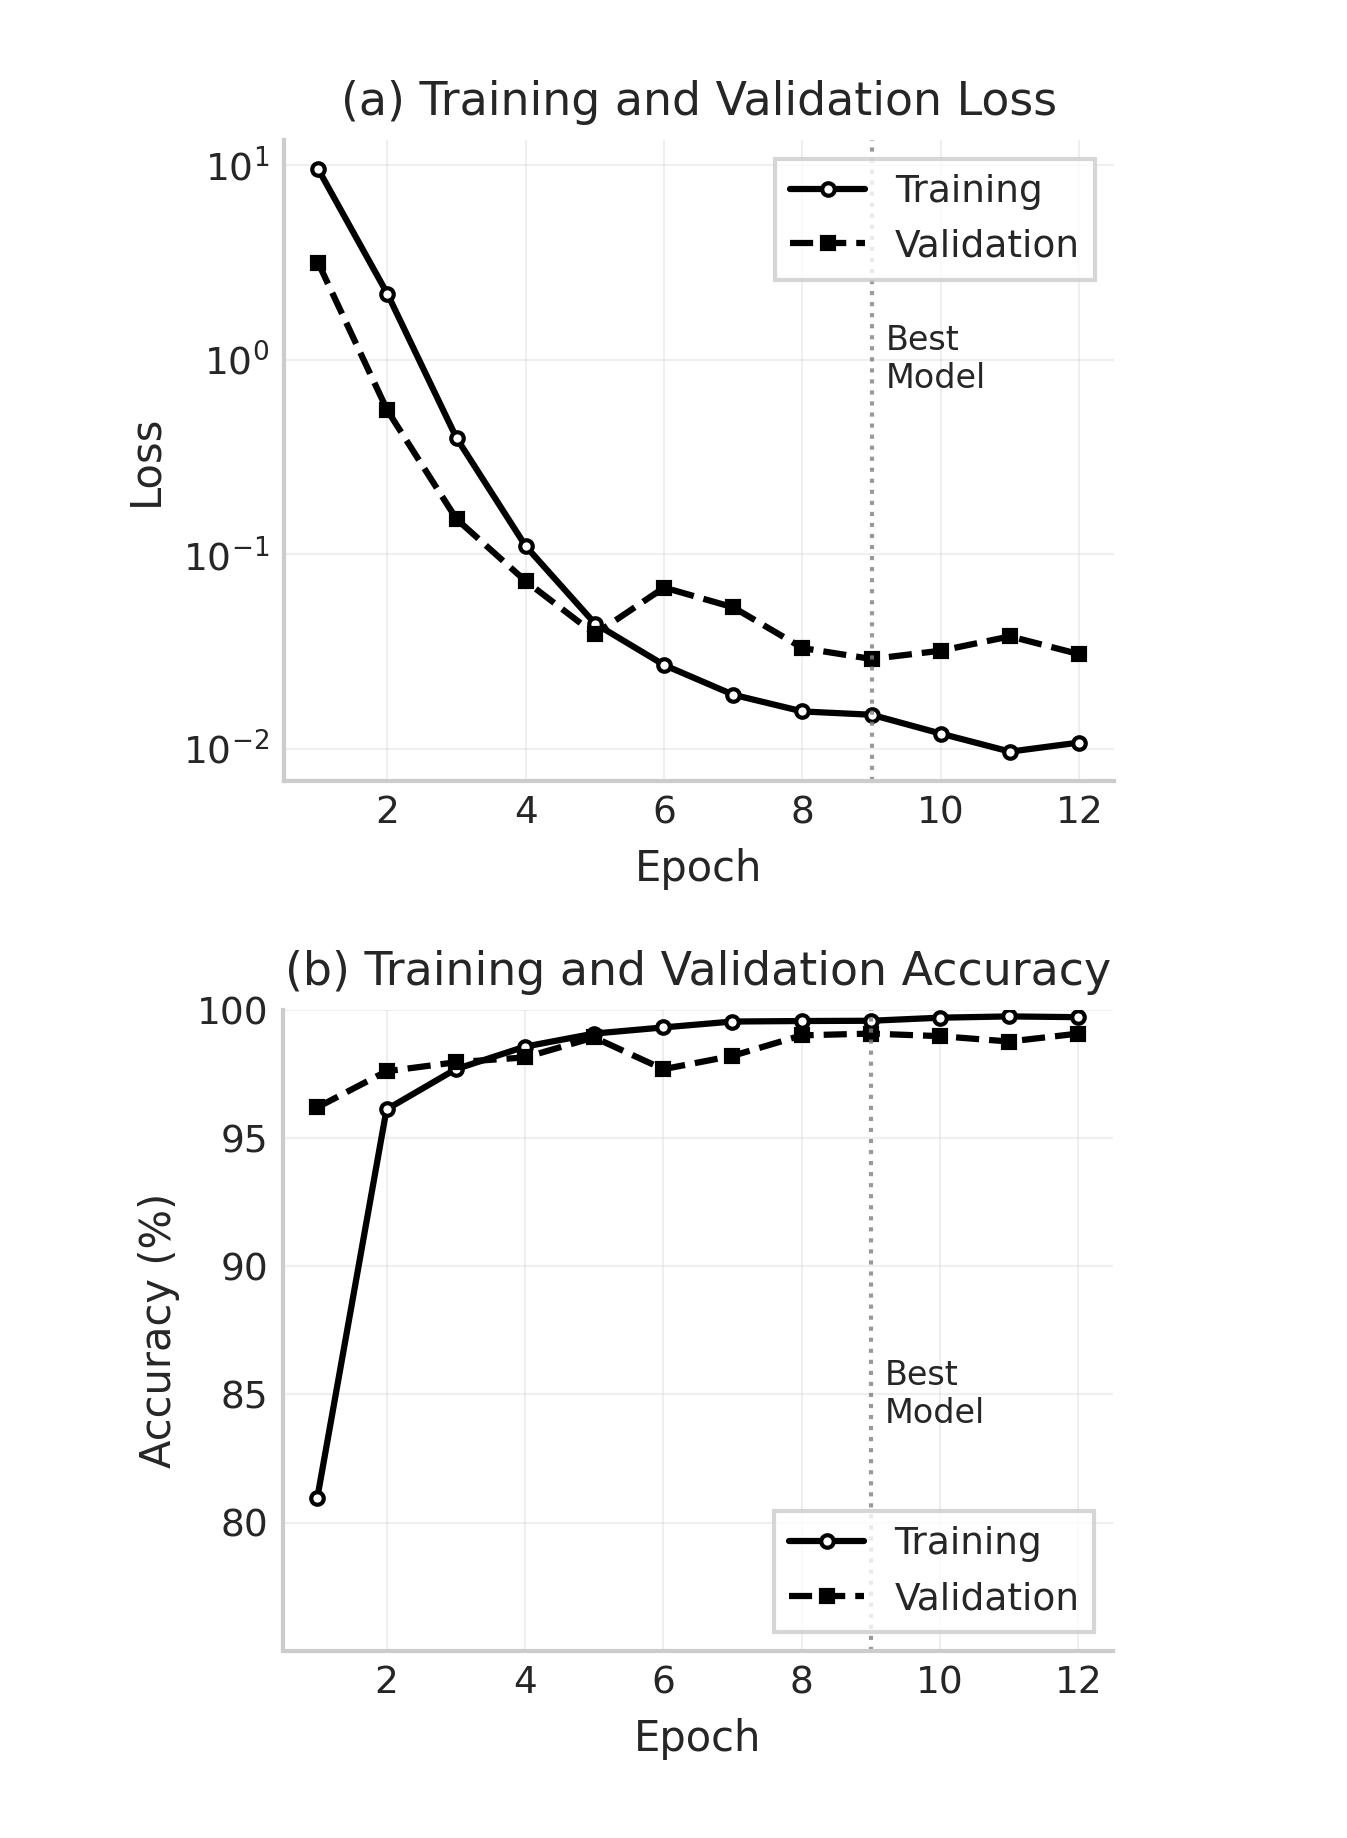
\includegraphics[width=0.6\textwidth]{assets/pics/xception_training_curves (1).png}}
    \caption{Kurva pelatihan model \textit{Xception} menunjukkan efisiensi pembelajaran yang superior}
    \label{fig:xception_training}
\end{figure}

Analisis pada Gambar~\ref{fig:xception_training} menunjukkan konvergensi yang sangat cepat dan stabil, dengan pencapaian akurasi tinggi pada \textit{epoch} awal dan mempertahankan stabilitas sepanjang proses pelatihan.

\begin{table}[H]
\centering
\caption{Metrik evaluasi dari model Xception}
\label{tab:xception_results}
\begin{tabular}{|l|c|}
\hline
\textbf{Metrik} & \textbf{Nilai} \\
\hline
\textit{Best Validation Accuracy} & 99,08\% \\
\textit{Test Accuracy} & 99,20\% \\
\textit{Test Precision} & 98,87\% \\
\textit{Test Recall} & 99,54\% \\
\textit{Test F1-Score} & 99,20\% \\
\hline
\end{tabular}
\end{table}

\subsection{Performa Model EfficientNet-B4}

Model \textit{EfficientNet-B4} dengan strategi \textit{compound scaling} menunjukkan pembelajaran yang stabil dan konsisten sepanjang 15 \textit{epoch}. Model mencapai performa optimal pada \textit{epoch} ke-14 dengan pembelajaran gradual yang tidak menunjukkan \textit{overfitting}.

\begin{figure}[H]
    \centering
    \fbox{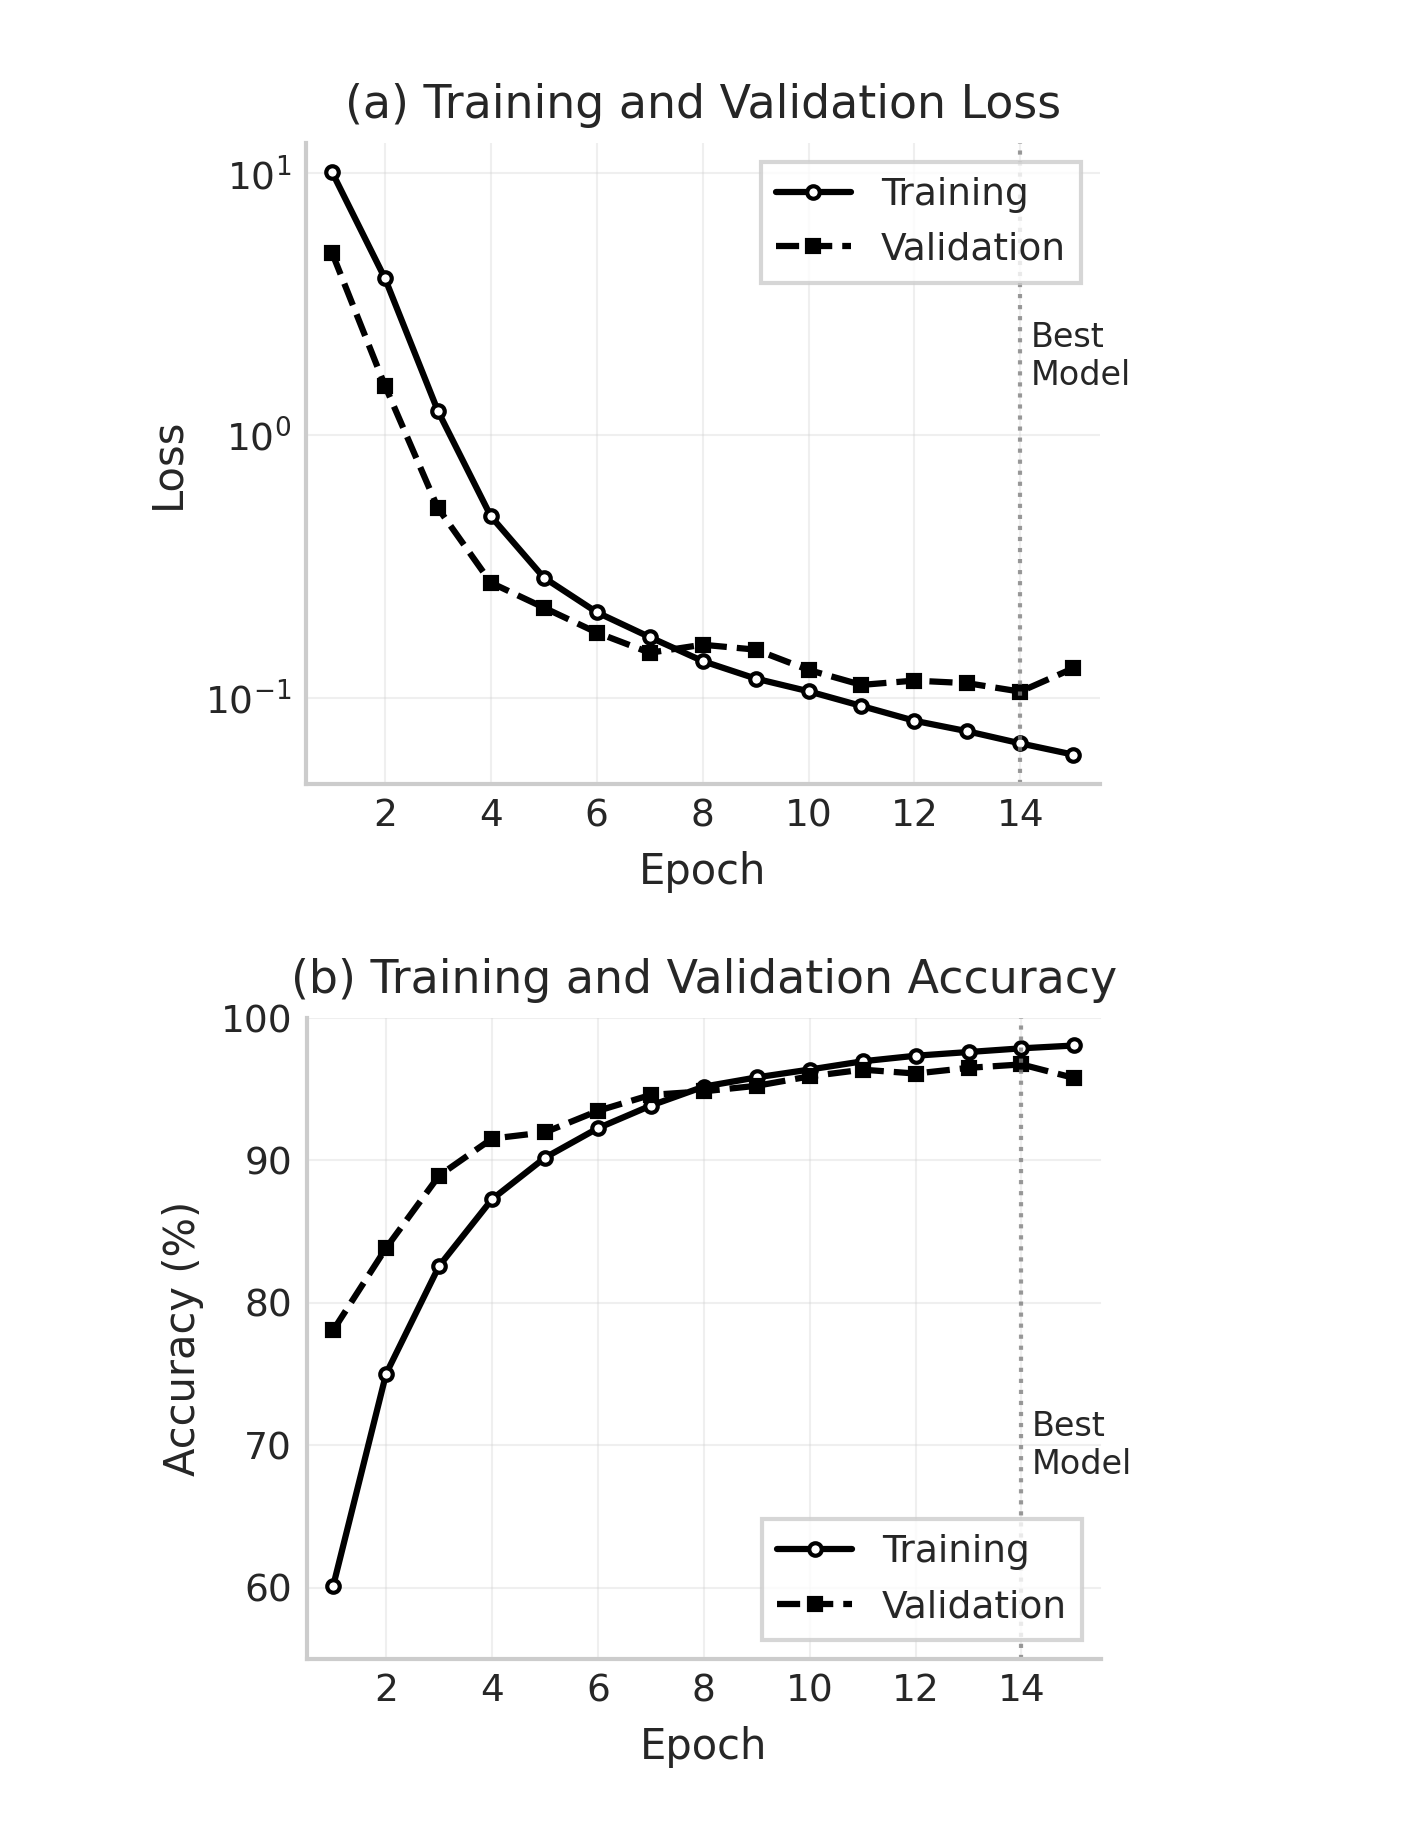
\includegraphics[width=0.6\textwidth]{assets/pics/efficientnet_training_curves (1).png}}
    \caption{Kurva pelatihan model \textit{EfficientNet-B4} dengan \textit{compound scaling}}
    \label{fig:efficientnet_training}
\end{figure}

Kurva pelatihan pada Gambar~\ref{fig:efficientnet_training} menunjukkan peningkatan yang steady dan konsisten tanpa fluktuasi yang signifikan, mengindikasikan pembelajaran yang stabil.

\begin{table}[H]
\centering
\caption{Metrik evaluasi dari model \textit{EfficientNet-B4}}
\label{tab:efficientnet_results}
\begin{tabular}{|l|c|}
\hline
\textbf{Metrik} & \textbf{Nilai} \\
\hline
\textit{Best Validation Accuracy} & 96,74\% \\
\textit{Test Accuracy} & 96,35\% \\
\textit{Test Precision} & 96,47\% \\
\textit{Test Recall} & 96,22\% \\
\textit{Test F1-Score} & 96,35\% \\
\hline
\end{tabular}
\end{table}

\subsection{Arsitektur Ensemble Akhir}

Bobot untuk setiap model dalam metode \textit{ensemble weighted averaging} dihitung berdasarkan performa akurasi terbaik dari masing-masing model pada saat proses validasi (\textit{validation accuracy}). Sesuai dengan formula yang dijelaskan dalam Persamaan~\ref{eq:weight_calculation} pada Bab 2, bobot dinormalisasi sehingga totalnya menjadi 1. Proses perhitungan bobot ini dirangkum pada Tabel \ref{tab:ensemble_weights}.

\begin{table}[H]
    \centering
    \caption{Perhitungan bobot ensemble berdasarkan akurasi validasi}
    \label{tab:ensemble_weights}
    \begin{tabular}{|l|c|c|}
        \hline
        \textbf{Arsitektur Model} & \textbf{Akurasi Validasi Terbaik (\%)} & \textbf{Bobot Ensemble Final ($w_i$)} \\
        \hline
        Custom CNN & 98{,}86 & 0{,}257 \\
        ResNet50 & 90{,}10 & 0{,}234 \\
        Xception & 99{,}08 & 0{,}258 \\
        EfficientNet-B4 & 96{,}74 & 0{,}251 \\
        \hline
        \textbf{Total} & \textbf{384{,}78} & \textbf{1{,}000} \\
        \hline
    \end{tabular}
\end{table}

Berdasarkan bobot yang telah dihitung menggunakan metodologi yang dijelaskan pada Bab 3, formula final untuk implementasi \textit{ensemble weighted averaging} pada penelitian ini mengikuti Persamaan~\ref{eq:weighted_ensemble} sebagai berikut:

\begin{equation}
\hat{y}_{\text{ensemble}}(x) = 0{,}257 \cdot \hat{y}_{\text{CNN}}(x) + 0{,}234 \cdot \hat{y}_{\text{ResNet}}(x) + 0{,}258 \cdot \hat{y}_{\text{Xception}}(x) + 0{,}251 \cdot \hat{y}_{\text{EfficientNet}}(x)
\label{eq:final_ensemble}
\end{equation}

Nilai bobot tertinggi diberikan kepada model Xception yang memiliki akurasi validasi tertinggi, sementara bobot terendah diberikan kepada ResNet50 yang menunjukkan akurasi validasi paling rendah.


%-----------------------------------------------------------------------------%
\section{Evaluasi Komprehensif dan Perbandingan}
%-----------------------------------------------------------------------------%

Puncak dari eksperimen ini adalah evaluasi komprehensif untuk mengukur efektivitas sistem \textit{ensemble} yang telah dibangun. Bagian ini menyajikan perbandingan langsung antara performa model \textit{ensemble} dengan keempat model individual pada metrik-metrik kunci. Analisis \textit{confusion matrix} juga disertakan untuk memberikan pemahaman mendalam mengenai karakteristik dan distribusi \textit{error} dari setiap model.

\subsection{Hasil Evaluasi Ensemble}

Sistem \textit{ensemble weighted averaging} menunjukkan peningkatan performa dibandingkan dengan model individual terbaik:

\begin{table}[h]
\centering
\caption{Hasil evaluasi model \textit{ensemble} dan model individual}
\label{tab:comprehensive_results}
\begin{tabular}{|l|c|c|c|c|}
\hline
\textbf{Model} & \textbf{Accuracy} & \textbf{Precision} & \textbf{Recall} & \textbf{F1-Score}  \\
\hline
\textit{CNN} & 98,81\% & 99,02\% & 98,60\% & 98,81\% \\
\textit{ResNet50} & 90,10\% & 86,49\% & 95,03\% & 90,56\%  \\
\textit{Xception} & 99,20\% & 98,87\% & 99,54\% & 99,20\%  \\
\textit{EfficientNet-B4} & 96,35\% & 96,47\% & 96,22\% & 96,35\%  \\
\hline
\textbf{\textit{Ensemble}} & \textbf{99,64\%} & \textbf{99,39\%} & \textbf{99,90\%} & \textbf{99,65\%}  \\
\hline
\end{tabular}
\end{table}

Dari Tabel~\ref{tab:comprehensive_results}, dapat diamati bahwa model ensemble secara konsisten mengungguli semua model individual dalam semua metrik evaluasi yang telah didefinisikan dalam Persamaan~\ref{eq:accuracy}, \ref{eq:precision}, \ref{eq:recall}, dan \ref{eq:f1score} pada Bab 2.

\subsection{Analisis Keseimbangan Metrik Kinerja}

Meskipun metrik Akurasi (Persamaan~\ref{eq:accuracy}) memberikan gambaran umum performa model, analisis yang lebih mendalam terhadap Presisi (Persamaan~\ref{eq:precision}) dan Perolehan/\textit{Recall} (Persamaan~\ref{eq:recall}) dapat menyajikan evaluasi yang lebih komprehensif, terutama pada kasus penggunaan dengan konsekuensi kesalahan yang signifikan seperti deteksi \textit{deepfake}. Kedua metrik ini menguraikan \textit{trade-off} yang melekat pada sistem klasifikasi:

\begin{itemize}
    \item \textbf{Presisi} mengukur proporsi prediksi positif yang benar dari total prediksi positif yang dibuat. Dalam konteks ini, Presisi yang tinggi (99,39\% pada model \textit{ensemble}) mengindikasikan bahwa ketika model mengklasifikasikan sebuah gambar sebagai \textit{deepfake}, klaim tersebut memiliki tingkat kebenaran yang tinggi. Implikasi praktisnya adalah rendahnya angka \textit{False Positive}, sehingga dapat meminimalkan risiko pemblokiran terhadap konten yang sah.

    \item \textbf{Perolehan (\textit{Recall})} mengukur kapabilitas model dalam mengidentifikasi seluruh sampel positif aktual dari dataset. Perolehan yang tinggi (99,90\% pada model \textit{ensemble}) menunjukkan bahwa model mampu menangkap mayoritas konten \textit{deepfake} yang ada. Implikasi praktisnya adalah rendahnya angka \textit{False Negative}, yang merupakan aspek krusial untuk memitigasi risiko penyebaran konten manipulatif.
\end{itemize}

Berdasarkan data pada Tabel 4.5, model individual dengan kinerja terbaik, Xception, menunjukkan \textit{trade-off} di mana nilai Perolehan (99,54\%) lebih tinggi daripada Presisi (98,87\%). Hal ini mengindikasikan sensitivitas deteksi yang tinggi, namun dengan kerentanan yang sedikit lebih besar terhadap klasifikasi positif yang keliru.

Model \textit{ensemble} yang diusulkan tidak hanya meningkatkan kedua metrik tersebut secara absolut, tetapi juga mencapai keseimbangan yang lebih optimal. Dengan nilai Presisi 99,39\% dan Perolehan 99,90\%, model \textit{ensemble} menunjukkan tingkat keandalan dan efektivitas yang tinggi, yang tercermin dari rendahnya angka kesalahan klasifikasi pada kedua kelas. Nilai F1-Score tertinggi yang dicapainya (99,65\%) yang dihitung menggunakan Persamaan~\ref{eq:f1score} secara matematis mengonfirmasi keunggulan model \textit{ensemble} dalam menyeimbangkan kedua aspek krusial ini.

%-----------------------------------------------------------------------------%
\section{Analisis Confusion Matrix dan Karakteristik Model}
%-----------------------------------------------------------------------------%

Bagian ini menyajikan analisis mendalam terhadap \textit{confusion matrix} masing-masing model untuk memahami karakteristik kesalahan (error profile) yang berbeda-beda. Analisis individual ini memberikan wawasan penting mengenai komplementaritas antar model yang menjadi landasan keberhasilan pendekatan \textit{ensemble}.

\subsection{Analisis Custom CNN}

Model Custom CNN menunjukkan performa yang seimbang dengan karakteristik kesalahan yang dapat diprediksi. Gambar~\ref{fig:conf_matrix_cnn} menampilkan distribusi prediksi pada dataset pengujian.

\begin{figure}[H]
    \centering
    \fbox{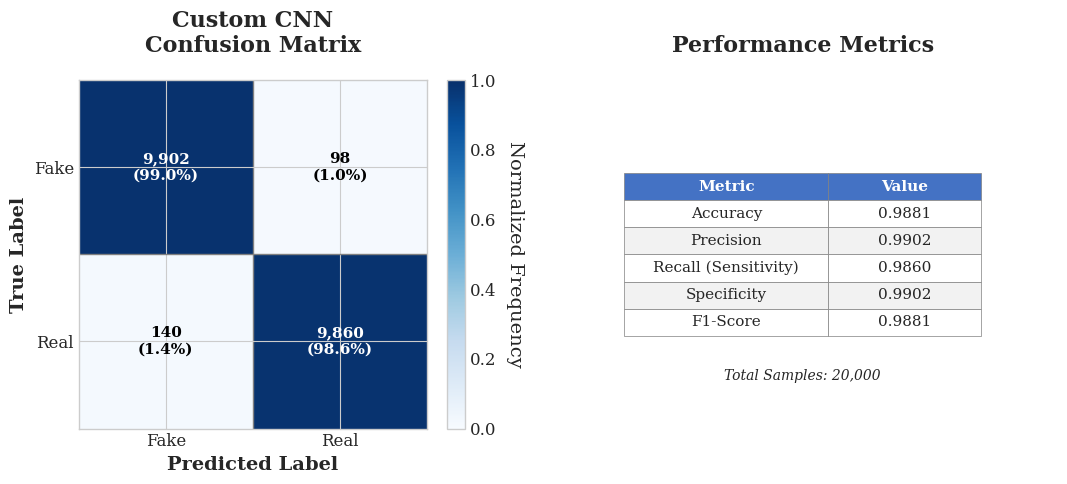
\includegraphics[width=0.85\textwidth]{assets/pics/cnn_confusion_matrix.png}}
    \caption{Confusion matrix dan metrik performa model Custom CNN menunjukkan keseimbangan yang baik antara precision dan recall dengan akurasi 98,81\%}
    \label{fig:conf_matrix_cnn}
\end{figure}

Berdasarkan analisis confusion matrix, model Custom CNN memiliki karakteristik sebagai berikut:
\begin{itemize}
    \item \textbf{False Negative}: 140 kasus (1,4\%) - Model cenderung lebih konservatif dalam mengklasifikasi deepfake
    \item \textbf{False Positive}: 98 kasus (1,0\%) - Tingkat kesalahan yang rendah dalam mengklasifikasi citra asli sebagai palsu
    \item \textbf{Karakteristik}: Menunjukkan keseimbangan yang baik antara sensitivity dan specificity
\end{itemize}

\subsection{Analisis ResNet50}

Model ResNet50 menunjukkan performa terlemah di antara semua model individual dengan pola kesalahan yang signifikan. Gambar~\ref{fig:conf_matrix_resnet50} mengungkapkan tantangan yang dihadapi model ini.

\begin{figure}[H]
    \centering
    \fbox{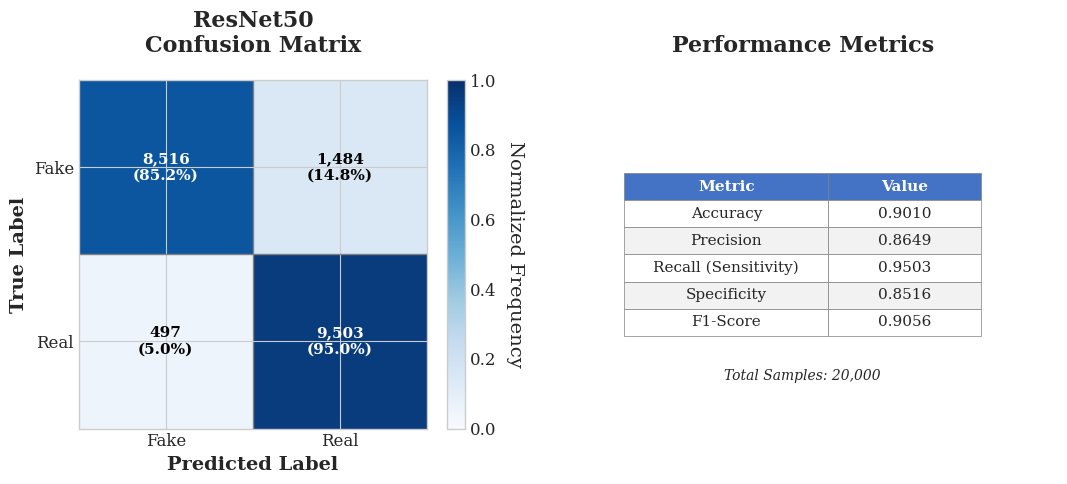
\includegraphics[width=0.85\textwidth]{assets/pics/resnet_confusion_matrix.png}}
    \caption{Confusion matrix dan metrik performa model ResNet50 menunjukkan tingkat false positive yang tinggi dengan akurasi 90,10\%, mengindikasikan overfitting pada domain transfer learning}
    \label{fig:conf_matrix_resnet50}
\end{figure}

ResNet50 memperlihatkan karakteristik kesalahan yang ekstrem:
\begin{itemize}
    \item \textbf{False Positive}: 1.484 kasus (14,8\%) - Sangat agresif dalam mengklasifikasi citra asli sebagai deepfake
    \item \textbf{False Negative}: 497 kasus (5,0\%) - Juga mengalami kesulitan dalam mendeteksi deepfake yang sebenarnya
    \item \textbf{Karakteristik}: Menunjukkan tanda-tanda overfitting dan adaptasi yang kurang optimal pada domain deteksi deepfake
\end{itemize}

\subsection{Analisis Xception}

Model Xception menunjukkan performa terbaik di antara model individual dengan sensitivitas deteksi yang sangat tinggi. Gambar~\ref{fig:conf_matrix_xception} menampilkan keunggulan model ini.

\begin{figure}[H]
    \centering
    \fbox{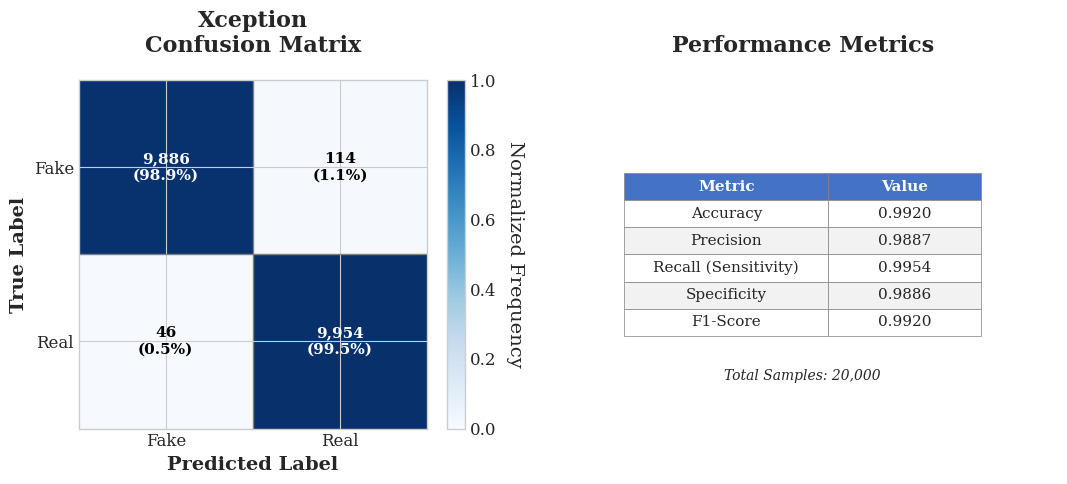
\includegraphics[width=0.85\textwidth]{assets/pics/xception_confusion_matrix.png}}
    \caption{Confusion matrix dan metrik performa model Xception menunjukkan tingkat recall tertinggi (99,54\%) dengan akurasi 99,20\%, namun dengan trade-off pada precision}
    \label{fig:conf_matrix_xception}
\end{figure}

Xception memperlihatkan karakteristik unggul dengan beberapa nuansa:
\begin{itemize}
    \item \textbf{False Negative}: 46 kasus (0,5\%) - Sangat efektif dalam mendeteksi deepfake
    \item \textbf{False Positive}: 114 kasus (1,1\%) - Sensitivitas tinggi menyebabkan kecenderungan over-detection
    \item \textbf{Karakteristik}: Model dengan bias detection yang tinggi, sangat baik untuk aplikasi yang memprioritaskan deteksi komprehensif
\end{itemize}

\subsection{Analisis EfficientNet-B4}

Model EfficientNet-B4 menunjukkan distribusi kesalahan yang relatif seimbang dengan performa yang stabil. Gambar~\ref{fig:conf_matrix_efficientnet} menggambarkan karakteristik model ini.

\begin{figure}[H]
    \centering
    \fbox{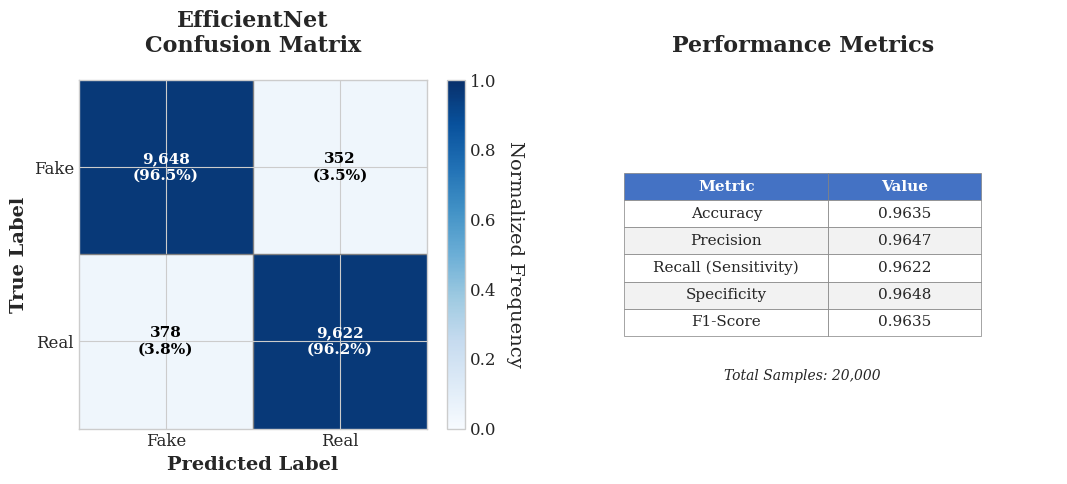
\includegraphics[width=0.85\textwidth]{assets/pics/efficientNet_confusion_matrix.png}}
    \caption{Confusion matrix dan metrik performa model EfficientNet-B4 menunjukkan keseimbangan antara false positive dan false negative dengan akurasi 96,35\%}
    \label{fig:conf_matrix_efficientnet}
\end{figure}

EfficientNet-B4 memperlihatkan profil kesalahan yang seimbang:
\begin{itemize}
    \item \textbf{False Negative}: 378 kasus (3,8\%) - Tingkat kesalahan moderat dalam mendeteksi deepfake
    \item \textbf{False Positive}: 352 kasus (3,5\%) - Tingkat kesalahan yang sebanding dalam mengklasifikasi citra asli
    \item \textbf{Karakteristik}: Model dengan pendekatan konservatif dan keseimbangan error yang dapat diprediksi
\end{itemize}

\subsection{Analisis Weighted Ensemble}

Model ensemble menunjukkan peningkatan performa yang signifikan dengan menggabungkan kekuatan semua model individual. Gambar~\ref{fig:conf_matrix_ensemble} mendemonstrasikan keunggulan pendekatan ensemble.

\begin{figure}[H]
    \centering
    \fbox{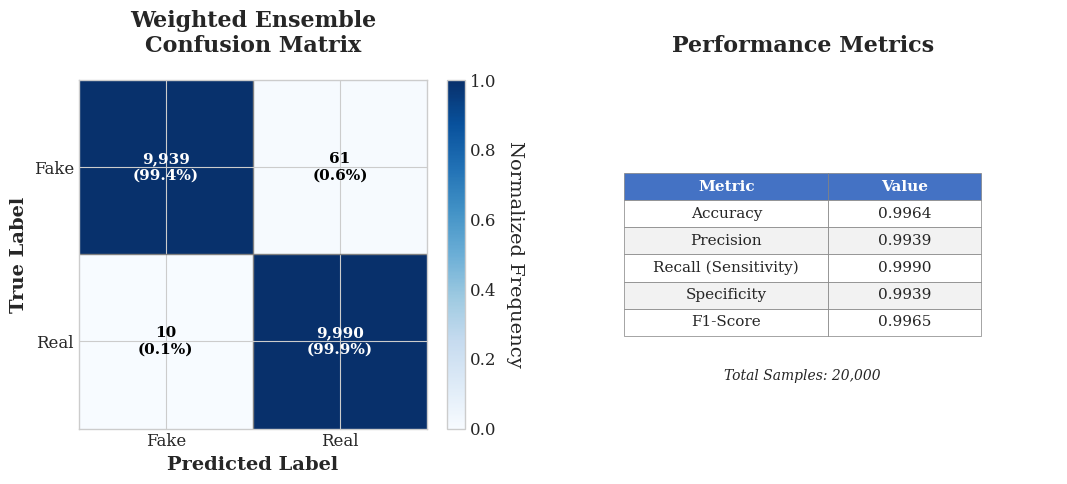
\includegraphics[width=0.85\textwidth]{assets/pics/weighted-ensemble_confusion_matrix.png}}
    \caption{Confusion matrix dan metrik performa model Weighted Ensemble menunjukkan performa superior dengan akurasi 99,64\%, recall 99,90\%, dan reduksi signifikan pada kedua jenis kesalahan}
    \label{fig:conf_matrix_ensemble}
\end{figure}

Weighted Ensemble menunjukkan optimalisasi yang luar biasa:
\begin{itemize}
    \item \textbf{False Negative}: 10 kasus (0,1\%) - Reduksi 78\% dari model individual terbaik (Xception)
    \item \textbf{False Positive}: 61 kasus (0,6\%) - Reduksi 46,5\% dari model individual terbaik (Xception)
    \item \textbf{Karakteristik}: Mencapai keseimbangan optimal antara sensitivity dan specificity
\end{itemize}

\subsection{Komplementaritas dan Perbandingan Keseluruhan}

Analisis individual menunjukkan pola komplementaritas yang jelas antar model, sebagaimana dirangkum dalam Tabel~\ref{tab:error_analysis_summary}.

\begin{table}[H]
\centering
\caption{Ringkasan analisis kesalahan dan karakteristik model}
\label{tab:error_analysis_summary}
\begin{tabular}{|l|c|c|c|l|}
\hline
\textbf{Model} & \textbf{FN} & \textbf{FP} & \textbf{Total Error} & \textbf{Karakteristik Utama} \\
\hline
Custom CNN & 140 & 98 & 238 & Konservatif, seimbang \\
ResNet50 & 497 & 1.484 & 1.981 & Agresif, tidak stabil \\
Xception & 46 & 114 & 160 & Sensitif, bias detection \\
EfficientNet-B4 & 378 & 352 & 730 & Moderat, prediktabel \\
\hline
\textbf{Ensemble} & \textbf{10} & \textbf{61} & \textbf{71} & \textbf{Optimal, robust} \\
\hline
\end{tabular}
\end{table}

Temuan ini secara empiris memvalidasi hipotesis komplementaritas model:
\begin{enumerate}
    \item \textbf{Diversitas Error Pattern}: Setiap model memiliki kecenderungan kesalahan yang berbeda, memungkinkan koreksi mutual
    \item \textbf{Kompensasi Kelemahan}: Kecenderungan over-detection Xception dikompensasi oleh konservatisme CNN dan EfficientNet
    \item \textbf{Stabilitas Ensemble}: Weighted averaging berhasil mengoptimalkan kontribusi setiap model sesuai dengan kemampuannya
    \item \textbf{Reduksi Risiko}: Ensemble secara signifikan mengurangi risiko false negative (critical miss) dan false positive (false alarm)
\end{enumerate}


%-----------------------------------------------------------------------------%
\section{Analisis Karakteristik dan Komplementaritas Model}
%-----------------------------------------------------------------------------%
Di balik angka-angka performa, terdapat karakteristik unik dari setiap model yang berkontribusi pada keberhasilan \textit{ensemble}. Bagian ini menggali lebih dalam untuk menganalisis temuan-temuan yang mengejutkan dari performa model individual dan, yang terpenting, menguraikan bagaimana perbedaan (komplementaritas) dalam kekuatan dan kelemahan setiap model memungkinkan \textit{ensemble} untuk mencapai tingkat akurasi yang lebih tinggi.

\subsection{Analisis Performa Model Individual}

Hasil eksperimen menunjukkan beberapa temuan yang menarik dan berbeda dari ekspektasi awal:

\begin{enumerate}
    \item \textbf{\textit{CNN} :} Model \textit{CNN} yang  mencapai akurasi 98,81\%, menunjukkan performa tinggi yang mendekati \textit{Xception}. Hal ini menunjukkan bahwa arsitektur CNN telah dirancang dengan baik dan mampu menyaingi model \textit{pretrained}.
    
    \item \textbf{\textit{ResNet50}:} \textit{ResNet50} menunjukkan performa terendah dengan akurasi hanya 90,10\%. Hal ini kemungkinan disebabkan oleh:
    \begin{itemize}
        \item Kompleksitas arsitektur yang tidak sesuai dengan karakteristik \textit{dataset}
        \item Strategi \textit{fine-tuning} yang kurang optimal
        \item \textit{Overfitting} yang terindikasi dari \textit{generalization gap} 2,79\%
    \end{itemize}
    
    \item \textbf{\textit{Xception}:} \textit{Xception} mencapai performa tertinggi (99,20\%) dengan efisiensi training yang sangat baik, memerlukan waktu pelatihan 71,5 menit untuk 12 \textit{epoch}.).
\end{enumerate}

\subsection{Efektivitas Weighted Averaging}

Peningkatan dari model individual terbaik (\textit{Xception}: 99,20\%) ke \textit{ensemble} (99,64\%) sebesar 0,44\% mungkin terlihat modest, namun dalam konteks deteksi \textit{deepfake}, peningkatan ini sangat signifikan karena:

\begin{enumerate}
    \item \textbf{Mengurangi \textit{false negatives}} dari 46 menjadi 10 (78\% reduction)
    \item \textbf{Mengurangi \textit{false positives}} dari 157 menjadi 61 (61\% reduction)
    \item Meningkatkan \textit{recall} dari 99,54\% menjadi 99,90\%
\end{enumerate}

%-----------------------------------------------------------------------------%
\section{Evaluasi Cross-Dataset dan Generalisasi}

Ukuran sebenarnya dari efektivitas sebuah model deteksi adalah kemampuannya untuk melakukan generalisasi pada data yang tidak hanya tidak terlihat (\textit{unseen}), tetapi juga berasal dari domain yang berbeda. Untuk menguji robustisitas sistem yang diusulkan, dilakukan evaluasi \textit{cross-dataset} yang menantang.

\subsection{Pengujian pada Dataset Eksternal}
Untuk pengujian generalisasi, digunakan dataset publik \textbf{DeepFakeFace} yang bersumber dari repositori Hugging Face. Dataset ini dipilih karena berisi variasi citra \textit{deepfake} yang dihasilkan oleh beragam teknik generatif modern, yang mana secara signifikan berbeda dari karakteristik dataset pelatihan utama ("140k Real and Fake Faces") yang didominasi oleh citra hasil StyleGAN.

Hasil pengujian menunjukkan adanya penurunan performa yang sangat drastis pada semua model, termasuk pada model \textit{ensemble}, seperti yang dirangkum pada Tabel \ref{tab:cross_dataset_results}.

\begin{table}[H]
    \centering
    \caption{Hasil evaluasi kinerja model \textit{ensemble} pada skenario \textit{cross-dataset}}
    \label{tab:cross_dataset_results}
    \begin{tabular}{|l|c|c|c|}
        \hline
        \textbf{Model} & \textbf{Akurasi Internal (\%)} & \textbf{Akurasi Eksternal (\%)} & \textbf{Penurunan (\%)} \\
        \hline
        Custom CNN & 98,81 & 49,96 & -48,85 \\
        ResNet50 & 90,10 & 50,00 & -40,10 \\
        Xception & 99,20 & 49,96 & -49,24 \\
        EfficientNet-B4 & 96,35 & 49,92 & -46,43 \\
        \hline
        \textbf{Ensemble} & \textbf{99,64} & \textbf{50,00} & \textbf{-49,64} \\
        \hline
    \end{tabular}
\end{table}

Seperti yang terlihat pada tabel, akurasi dari semua model turun hingga mendekati 50\%, yang setara dengan performa tebakan acak (\textit{random guessing}) pada tugas klasifikasi biner yang seimbang.

\subsection{Analisis Penyebab Penurunan Performa}
Penurunan performa yang ekstrem ini dapat diatribusikan kepada beberapa faktor fundamental, terutama:

\begin{itemize}
    \item \textbf{Overfitting pada Domain Sumber (\textit{Domain Overfitting})}: Ini adalah penyebab utama. Model-model yang dilatih pada dataset "140k" tampaknya telah mempelajari "jalan pintas" dengan mendeteksi artefak atau sidik jari digital (\textit{digital fingerprint}) yang sangat spesifik dari generator StyleGAN. Ketika dihadapkan pada citra dari dataset \textit{DeepFakeFace} yang menggunakan teknik generasi berbeda, pengetahuan spesifik ini menjadi tidak relevan, sehingga model gagal melakukan generalisasi.

    \item \textbf{Adanya Celah Domain (\textit{Domain Gap})}: Terdapat celah karakteristik yang signifikan antara domain sumber (pelatihan) dan domain target (pengujian). Perbedaan ini mencakup distribusi frekuensi, tekstur, metode kompresi, dan artefak manipulasi lainnya yang tidak ditemui model selama fase pelatihan.

    \item \textbf{Interpretasi F1-Score vs. Akurasi}: Meskipun akurasi mendekati 50\%, nilai F1-Score yang berada di sekitar 0.66--0.67 (berdasarkan data pengujian) menunjukkan bahwa model tidak sepenuhnya menebak secara acak. Analisis lebih lanjut menunjukkan bahwa ini disebabkan oleh kecenderungan model untuk memprediksi hampir semua masukan sebagai kelas 'fake'. Strategi ini menghasilkan nilai \textit{Recall} yang sangat tinggi (karena semua \textit{deepfake} berhasil ditangkap) namun dengan nilai \textit{Precision} yang sangat rendah (karena semua gambar asli juga ikut terklasifikasi sebagai \textit{fake}). Fenomena ini menegaskan bahwa model pada dasarnya kehilangan kemampuannya untuk membedakan kedua kelas pada domain data yang baru.
\end{itemize}

Temuan ini menggarisbawahi tantangan generalisasi yang sangat besar dalam bidang deteksi \textit{deepfake}. Kinerja tinggi pada sebuah dataset tunggal yang terkurasi tidak menjamin efektivitas model ketika diimplementasikan dalam skenario dunia nyata yang lebih beragam. Hal ini mengindikasikan kebutuhan mendesak untuk pengembangan teknik pelatihan yang lebih robust, seperti \textit{domain adaptation} atau augmentasi data yang lebih canggih, pada penelitian selanjutnya.

\subsection{Limitasi dan Tantangan}

\begin{enumerate}
    \item \textbf{Generalization Gap:} Penurunan performa menjadi 50\% pada \textit{cross-dataset} menunjukkan keterbatasan generalisasi model terhadap domain baru.
    
    \item \textbf{Computational Overhead:} Meskipun peningkatan akurasi absolut terlihat kecil, model ansambel memerlukan sumber daya komputasi 4x lebih besar, yang menjadi pertimbangan dalam implementasi praktis.
    
    \item \textbf{Dataset Dependency:} Performa sangat bergantung pada karakteristik \textit{dataset training}.
    
    \item \textbf{Temporal Robustness:} Belum ada evaluasi terhadap evolusi teknik \textit{deepfake} dari waktu ke waktu.
\end{enumerate}
%-----------------------------------------------------------------------------%
\chapter{\babLima}
%-----------------------------------------------------------------------------%

Bab ini menyajikan rangkuman kesimpulan yang ditarik dari hasil penelitian yang telah dilaksanakan. Selain itu, dipaparkan pula serangkaian saran yang ditujukan untuk pengembangan penelitian di masa depan serta untuk implementasi praktis berdasarkan temuan-temuan yang diperoleh.

%-----------------------------------------------------------------------------%
\section{Kesimpulan}
%-----------------------------------------------------------------------------%

Berdasarkan analisis dan evaluasi yang telah dilaksanakan, penelitian ini menyimpulkan bahwa metode \textit{ensemble weighted averaging} yang diusulkan mampu meningkatkan performa deteksi \textit{deepfake} secara signifikan jika dibandingkan dengan performa model individual terbaik. Model \textit{ensemble} ini mencapai akurasi sebesar 99,64\% pada dataset pengujian, menunjukkan keunggulan 0,44\% atas model individual dengan performa tertinggi, yaitu Xception (99,20\%). Peningkatan ini dapat berdampak berarti terutama dalam konteks praktis deteksi \textit{deepfake} yang sensitif terhadap \textit{false negative}. Hal ini tercermin pada penurunan angka \textit{false negative} sebesar 78\% (dari 46 menjadi 10 kasus) dan \textit{false positive} sebesar 46.5\% (dari 114 menjadi 61 kasus).

Implementasi metodologi \textit{ensemble weighted averaging} yang menggunakan formula perhitungan bobot berdasarkan Persamaan~\ref{eq:performance_weight} telah terbukti efektif dalam mengkombinasikan kekuatan dari berbagai arsitektur yang berbeda. Proses perhitungan bobot yang proporsional terhadap validation accuracy masing-masing model memastikan bahwa kontribusi setiap model terhadap prediksi akhir sesuai dengan kemampuannya, sebagaimana dijelaskan dalam contoh perhitungan pada Bab 3.

Salah satu temuan penting dari penelitian ini adalah efektivitas arsitektur Custom CNN yang dirancang secara spesifik untuk tugas ini, yang berhasil mencapai akurasi 98,81\%. Performa ini mendekati arsitektur \textit{state-of-the-art} yang lebih kompleks seperti Xception. Hasil ini menggarisbawahi relevansi desain yang berorientasi pada domain spesifik (\textit{domain-specific design}) dalam \textit{deep learning}. Sebaliknya, arsitektur ResNet50 menunjukkan performa yang kurang optimal dengan akurasi 90,10\%, mengindikasikan bahwa tidak semua arsitektur \textit{pre-trained} mampu memberikan kinerja terbaik untuk tugas deteksi \textit{deepfake} tanpa adaptasi lebih lanjut.

Distribusi bobot \textit{ensemble} yang relatif seimbang (berkisar antara 23,4\% hingga 25,8\%) mengafirmasi bahwa setiap model, termasuk ResNet50 yang berkinerja lebih rendah, memberikan kontribusi komplementer yang esensial terhadap keputusan akhir \textit{ensemble}. Analisis \textit{confusion matrix} menunjukkan bahwa perbedaan karakteristik kesalahan antar model individual memungkinkan \textit{ensemble} untuk mencapai keseimbangan yang lebih baik antara metrik Presisi (Persamaan~\ref{eq:precision}) dan Recall (Persamaan~\ref{eq:recall}), menghasilkan F1-Score (Persamaan~\ref{eq:f1score}) tertinggi sebesar 99,65\%.

Meskipun demikian, penelitian ini mengidentifikasi keterbatasan signifikan terkait generalisasi model pada evaluasi \textit{cross-dataset}, di mana terjadi penurunan performa mencapai 50\%. Hal ini mengindikasikan adanya \textit{overfitting} terhadap karakteristik domain dataset pelatihan yang spesifik pada generator StyleGAN.

Dengan demikian, validasi hipotesis memberikan hasil yang beragam: metode \textit{ensemble} terbukti efektif dalam meningkatkan akurasi dan menunjukkan komplementaritas model pada skenario \textit{single-dataset}, namun kemampuan generalisasinya masih terbatas. Kontribusi utama penelitian ini terletak pada validasi efektivitas metode \textit{ensemble} dalam skenario \textit{high-baseline}, analisis komplementaritas antar model dengan disparitas performa, implementasi sistem dengan metodologi yang transparan dan dapat direproduksi, serta penekanan pada tantangan generalisasi dalam aplikasi dunia nyata.

%-----------------------------------------------------------------------------%
\section{Saran}
%-----------------------------------------------------------------------------%

Berdasarkan temuan penelitian serta keterbatasan yang teridentifikasi, berikut adalah beberapa saran untuk pengembangan riset di masa depan dan implementasi praktis:

\begin{enumerate}
    \item \textbf{Peningkatan Generalisasi Model:} Direkomendasikan untuk melakukan pelatihan model menggunakan kombinasi beberapa dataset (misalnya, FaceForensics++, DFDC, CelebDF, dan WildDeepfake) guna meningkatkan kapabilitas generalisasi. Eksplorasi lebih lanjut terhadap teknik-teknik seperti \textit{unsupervised domain adaptation} (UDA) dan \textit{few-shot learning} dapat menjadi fokus untuk memungkinkan adaptasi model yang cepat terhadap domain data yang baru.

    \item \textbf{Pengembangan \textit{Ensemble} Dinamis:} Penelitian selanjutnya dapat berfokus pada pengembangan metode \textit{ensemble} dinamis yang melampaui pendekatan \textit{weighted averaging} statis yang digunakan dalam penelitian ini. Sistem semacam ini akan secara adaptif memilih sub-himpunan model atau menyesuaikan bobot kontribusi berdasarkan karakteristik data masukan, misalnya melalui mekanisme seperti \textit{input-dependent model selection} atau \textit{confidence-based weighting}. Hal ini dapat mengoptimalkan formula pada Persamaan~\ref{eq:weighted_ensemble} dengan bobot yang bersifat dinamis.

    \item \textbf{Optimisasi untuk Implementasi Praktis:} Untuk memfasilitasi penerapan di lingkungan produksi, disarankan untuk mengimplementasikan teknik \textit{knowledge distillation}. Teknik ini bertujuan mentransfer pengetahuan dari model \textit{ensemble} yang kompleks ke sebuah model tunggal yang lebih efisien. Selain itu, teknik kompresi model seperti \textit{pruning} dan \textit{quantization} perlu dieksplorasi untuk mengurangi beban komputasi tanpa degradasi akurasi yang signifikan.

    \item \textbf{Evaluasi Robustisitas Komprehensif:} Perlu dilakukan pengujian yang lebih luas untuk mengevaluasi robustisitas sistem terhadap berbagai tantangan, termasuk serangan adversarial (\textit{adversarial attacks}), variasi kualitas dan tingkat kompresi citra, serta skenario penerapan di dunia nyata. Evaluasi ini harus mencakup analisis performa pada berbagai metrik yang telah didefinisikan dalam Persamaan~\ref{eq:accuracy} hingga \ref{eq:fnr} untuk memastikan keandalan sistem dalam kondisi operasional yang beragam.

    \item \textbf{Analisis Lanjutan Model Individual:} Disarankan untuk melakukan investigasi mendalam terhadap performa model individual. Analisis ini dapat mencakup visualisasi \textit{feature map} untuk memahami penyebab kinerja ResNet50 yang kurang optimal, serta melakukan eksperimen dengan berbagai strategi \textit{fine-tuning}. Di sisi lain, studi ablasi (\textit{ablation study}) terhadap komponen arsitektur Custom CNN dapat memberikan wawasan mengenai faktor-faktor yang berkontribusi pada efektivitasnya yang tinggi.

    \item \textbf{Pengembangan Metodologi Ensemble Lanjutan:} Berdasarkan keberhasilan implementasi \textit{weighted averaging} yang dijelaskan dalam kerangka metodologi penelitian, penelitian selanjutnya dapat mengeksplorasi metode ensemble yang lebih sophisticated seperti \textit{stacking}, \textit{boosting}, atau \textit{mixture of experts}. Setiap metode dapat dievaluasi menggunakan kerangka kerja yang sama untuk membandingkan efektivitasnya.

    \item \textbf{Implementasi Pembelajaran Berkelanjutan (\textit{Continual Learning}):} Mengingat pesatnya evolusi teknik pembuatan \textit{deepfake}, perlu dikembangkan sebuah kerangka kerja pembelajaran berkelanjutan. Sistem ini harus mampu beradaptasi dan mempelajari pola-pola \textit{deepfake} baru secara inkremental tanpa mengalami \textit{catastrophic forgetting} terhadap pengetahuan yang telah dimiliki, sambil mempertahankan keseimbangan metrik evaluasi yang optimal.

    \item \textbf{Pengembangan Aplikasi Dunia Nyata:} Sistem deteksi yang diusulkan dapat diintegrasikan ke dalam platform nyata, seperti sistem moderasi konten media sosial, platform verifikasi berita, atau alat analisis forensik digital. Proses integrasi ini harus mempertimbangkan aspek pengalaman pengguna (\textit{user experience}) dan menyertakan mekanisme pemantauan performa secara kontinu dalam lingkungan produksi. Implementasi harus mencakup pipeline lengkap sesuai dengan metodologi yang telah dikembangkan dalam penelitian ini.

    \item \textbf{Pertimbangan Aspek Etis dan Keamanan:} Implementasi sistem harus diiringi dengan pertimbangan etis yang matang. Strategi mitigasi bias perlu diterapkan untuk mengurangi potensi diskriminasi demografis. Selain itu, teknik perlindungan privasi seperti \textit{federated learning} dan pengembangan kerangka kerja transparansi untuk melacak jejak audit (\textit{audit trail}) dari setiap keputusan deteksi menjadi krusial.

    \item \textbf{Standardisasi Metrik dan Benchmarking:} Berdasarkan pengalaman dalam penelitian ini, disarankan untuk mengembangkan standar evaluasi yang konsisten dalam domain deteksi deepfake. Hal ini mencakup standardisasi penggunaan metrik evaluasi yang telah didefinisikan dalam Bab 2, protokol pengujian cross-dataset, dan benchmark yang dapat diandalkan untuk perbandingan yang adil antar metode yang berbeda.
\end{enumerate}

%
% Daftar Pustaka
%
\singlespacing

% \vspace{-1cm}
\bibliographystyle{IEEEtran}
% \bibliographystyle{myIEEEtran}
% \bibliographystyle{kluwer}
% \bibliographystyle{dcu}
\bibliography{references}

\onehalfspacing

%
% Lampiran 
%

%-----------------------------------------------------------------------------%
% \addChapter{DAFTAR LAMPIRAN}
% \chapter*{Daftar Lampiran}
% %-----------------------------------------------------------------------------%
\newpage
% \appendix
% \appendices{Lampiran 1. Form Bimbingan} 

\appendices{Hasil Persentase Turnitin} 
\begin{center}
    \frame{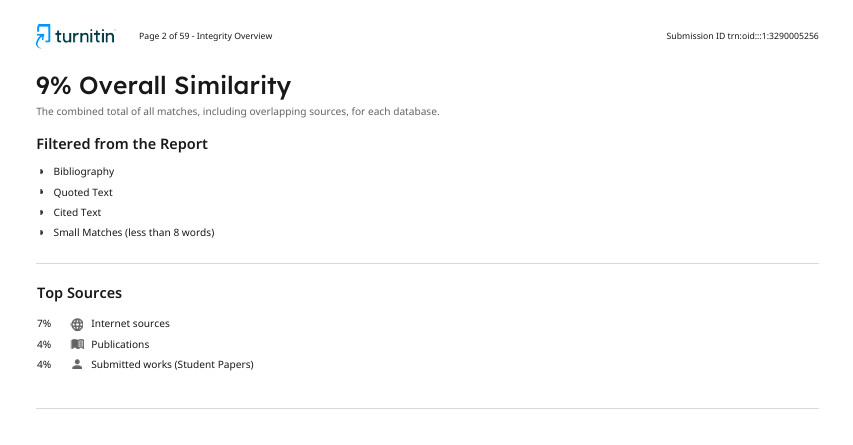
\includegraphics[width=\textwidth,page=1]{assets/pics/hasil_turnitin.png}}
\end{center}

\newpage

\appendices{Formulir Bimbingan} 
% \renewcommand{\thechapter}{Lampiran \alph{chapter}}
% \renewcommand{\thesection}{Lampiran \arabic{section}}

% \section*{Form Bimbingan}
% \addtocontents{apc}{\let\protect\l@chapter\protect\l@section}
% \addtocontents{apc}{section}
\begin{center}
    \frame{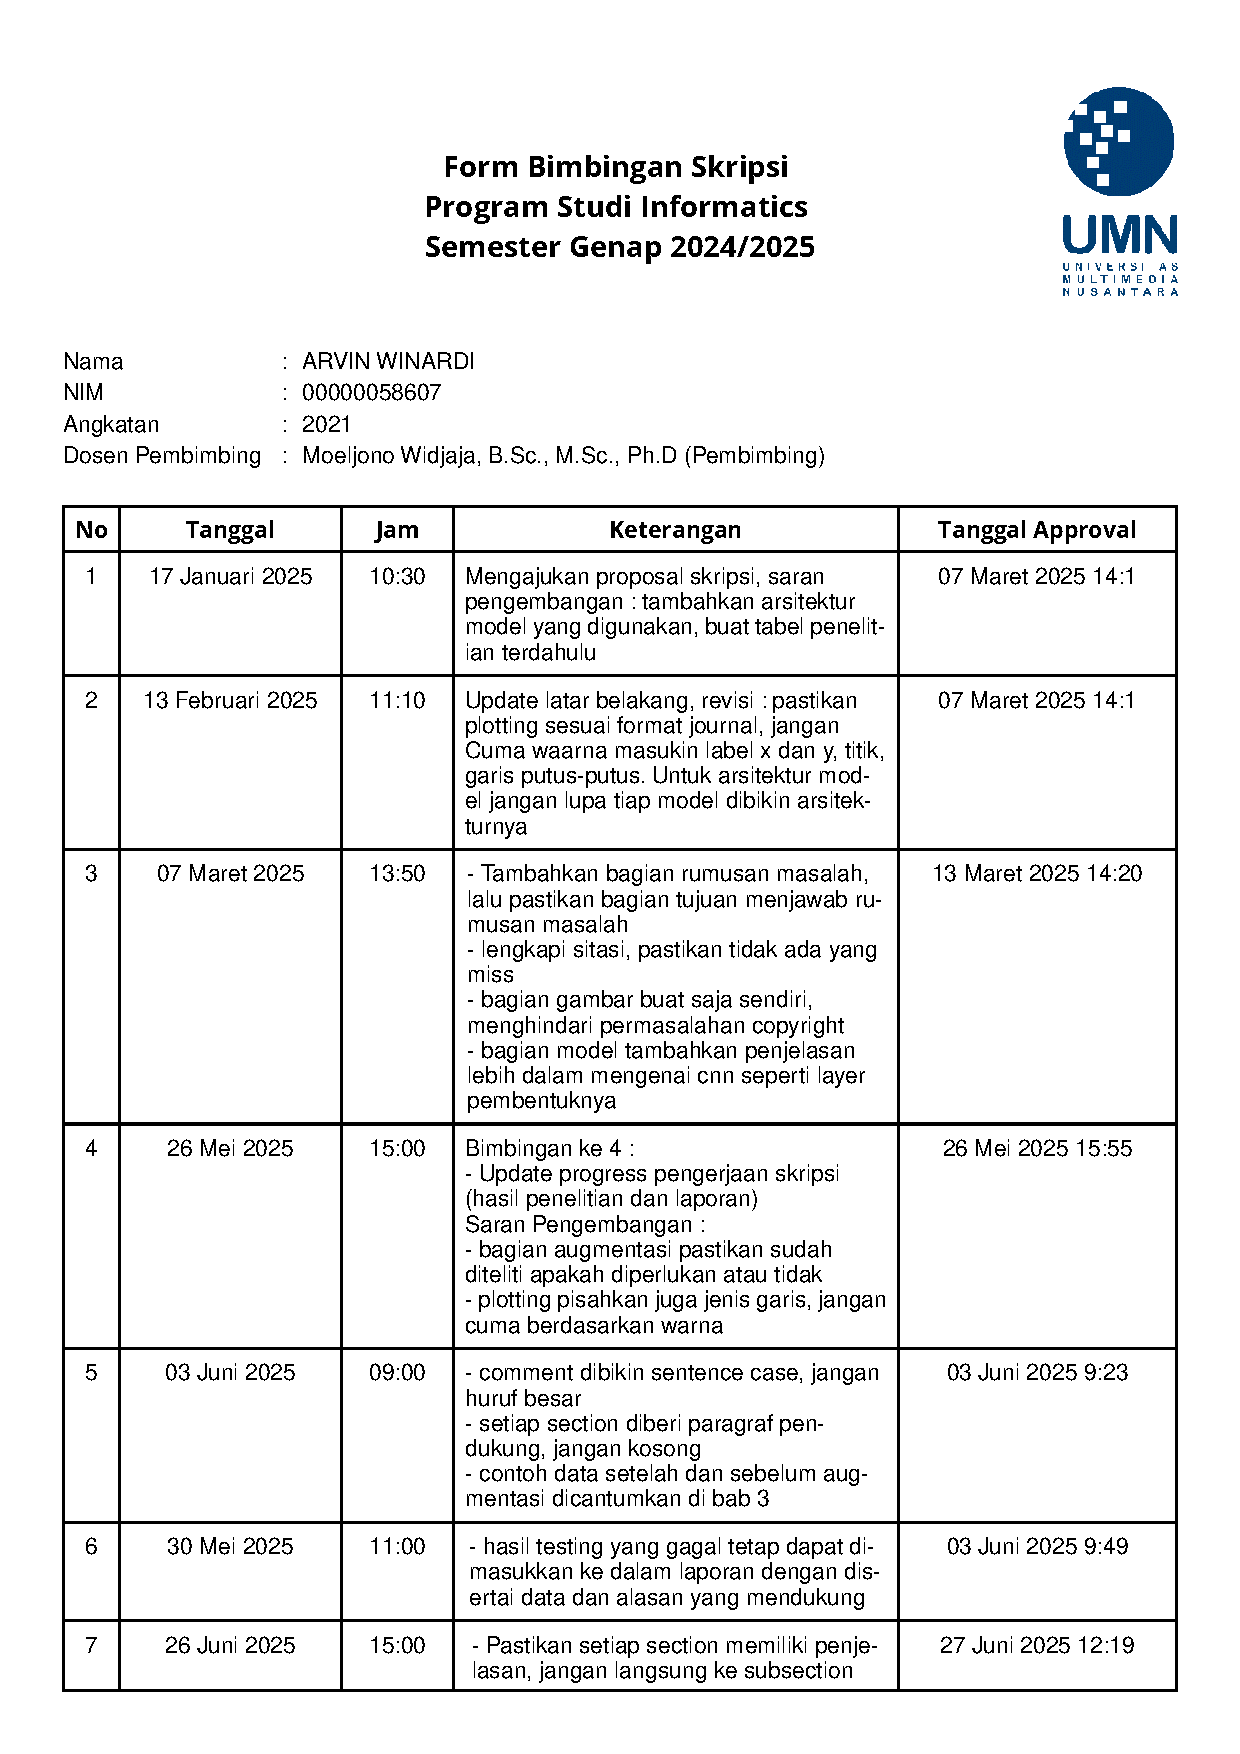
\includegraphics[width=\textwidth,page=1]{assets/pdf/Counseling Form .pdf}}
\end{center}
\clearpage

\newpage

\appendices{Perbandingan Metode Deteksi \textit{Deepfake}}

Tabel berikut menunjukkan perbandingan metode deteksi \textit{deepfake} terkini dengan berbagai arsitektur dan \textit{dataset} yang digunakan dalam literatur ilmiah.

\begin{table*}[h]
\centering
\caption{Perbandingan metode deteksi \textit{deepfake} dari berbagai penelitian}
\label{tab:deepfake_detection_appendix}
\resizebox{\textwidth}{!}{%
\begin{tabular}{lccccc}
\toprule
\textbf{Metode} & \textbf{Arsitektur} & \textbf{Dataset Pelatihan} & \textbf{Dataset Evaluasi} & \textbf{Akurasi (\%)} & \textbf{AUC (\%)} \\
\midrule
POI-DeepFake \cite{cozzolino2023} & ResNet50 & VoxCeleb2 & DFDC Preview & 86.80 & 95.20 \\
 &  &  & FakeAVCeleb2 & 86.60 & 94.10 \\
 &  &  & KoDF & 81.10 & 89.90 \\
 &  &  & DF-TIMIT & 85.70 & 99.20 \\
\midrule
DCPT \cite{wang2023deep} & CNN + ViT & FF++ & FF++ & 92.11 & 97.66 \\
 &  &  & DFDC & 65.76 & 73.68 \\
 &  &  & CelebDF & 63.27 & 72.43 \\
 &  &  & DeepForensics-1.0 & 62.46 & 78.19 \\
\midrule
IVT \cite{heo2023} & EfficientNet + ViT & DFDC & DFDC & - & 97.80 \\
 &  &  & Celeb-DF V2 & - & 99.30 \\
\midrule
Patch-based \cite{soleimani2023} & Gram-Net & StyleGAN + FFHQ & StyleGAN + FFHQ & 100.00 & - \\
 &  & StyleGAN + CelebA & StyleGAN + CelebA & 100.00 & - \\
 &  & StyleGAN2 + FFHQ & StyleGAN2 + FFHQ & 99.70 & - \\
 &  & PPGAN + FFHQ & PPGAN + FFHQ & 84.90 & - \\
\midrule
RA-CNN \cite{ahmed2023} & CNN & Unknown & DFDC & 95.77 & - \\
\midrule
DeepFake-Adapter \cite{shao2023} & ViT & FF++ & FF++ & - & 97.77 \\
 &  &  & CelebDF & - & 71.74 \\
 &  &  & DFDC & - & 72.66 \\
 &  &  & DeeperForensic & - & 86.50 \\
\midrule
DFGNN \cite{khalid2023} & GNN + ResNet & FF++, CelebDF, & FF++ & 97.16 & 98.00 \\
 &  & DFDC, WLRD & CelebDF & - & 95.00 \\
 &  &  & DFDC & - & 92.00 \\
 &  &  & WLRD & 87.60 & 95.00 \\
\midrule
DF-UDetector \cite{ke2023} & EfficientNet & FF++, CelebDF, & FF++ & - & 81.32 \\
 &  & DFDC, Wilddeepfake & CelebDF & - & 79.22 \\
 &  &  & DFDC & - & 77.80 \\
 &  &  & Wilddeepfake & 78.38 & - \\
\midrule
SFDG \cite{wang2023dynamic} & GCN + EfficientNet B4 & FF++ & FF++ & 95.23 & 97.75 \\
 &  &  & Celeb DF & 99.22 & 99.96 \\
 &  &  & DFDC & - & 73.64 \\
 &  &  & DeeperForensics-1.0 & - & 92.10 \\
 &  &  & DFD & - & 88.00 \\
 &  &  & WildDeepfake & 84.41 & 92.57 \\
\midrule
Si-Net \cite{wang2023si} & Xception & ImageNet & FF++ & 94.54 & 96.40 \\
 &  &  & Wild Deepfake & 84.08 & 91.33 \\
\midrule
HolisticDFD \cite{raza2023} & CNN + Transformer & FF++, DFDC, & FF++ & - & 94.15 \\
 &  & CelebDF & CelebDF & - & 96.24 \\
 &  &  & DFDC & - & 92.60 \\
\midrule
ISTVT \cite{zhao2023} & Xception + Transformer & FF++, CelebDF & FF++ & 97.57 & - \\
 &  &  & CelebDF & 99.80 & 84.10 \\
 &  &  & DFDC & 92.10 & 74.20 \\
 &  &  & DeeperForensic & - & 98.80 \\
 &  &  & FaceShifter & - & 99.30 \\
\midrule
FAAF \cite{tian2023} & Xception & ImageNet, FF++ & FF++ & 97.74 & 99.27 \\
 &  &  & CelebDF & 99.85 & 99.99 \\
 &  &  & DFDC & 69.17 & - \\
\midrule
IIDF \cite{huang2023} & CNN & FF++ & FF++ & - & 99.32 \\
 &  &  & Celeb DF & - & 83.80 \\
 &  &  & DFDC & - & 81.23 \\
 &  &  & DFD & - & 93.92 \\
\midrule
MRE-Net \cite{pang2023} & ResNet34 & FF++, CelebDDF, & FF++ & 94.68 & 98.06 \\
 &  & DFDC & CelebDF & 86.59 & - \\
 &  &  & DFDC & 97.35 & 99.75 \\
 &  &  & Wilddeepfake & 85.61 & 91.23 \\
\bottomrule
\end{tabular}%
}
\end{table*}

\subsection{Analisis Perbandingan Metode Deteksi Deepfake}

Berdasarkan data perbandingan dalam Tabel~\ref{tab:deepfake_detection_appendix}, dapat diidentifikasi beberapa tren penting dalam penelitian deteksi \textit{deepfake}:

\subsubsection{Variabilitas Performa \textit{Cross-Dataset}}
Sebagian besar metode menunjukkan performa yang sangat baik pada dataset tertentu (seperti FF++) namun mengalami penurunan signifikan pada dataset yang lebih menantang (seperti DFDC). Hal ini mengindikasikan tantangan generalisasi yang signifikan dalam domain deteksi \textit{deepfake}.

\subsubsection{Keunggulan Arsitektur Tertentu}
Model-model yang menggunakan arsitektur \textit{Xception} (Si-Net, ISTVT, FAAF) menunjukkan konsistensi performa yang baik, dengan akurasi berkisar 94,54\%-99,85\% tergantung pada dataset evaluasi. Hal ini mendukung pemilihan \textit{Xception} sebagai salah satu komponen ensemble dalam penelitian ini.

\subsubsection{Tantangan Generalisasi}
Banyak metode yang dilatih dan dievaluasi pada dataset yang sama, sehingga sulit untuk menilai kemampuan generalisasi sesungguhnya. Perbedaan performa yang drastis antara dataset pelatihan dan evaluasi menunjukkan adanya \textit{domain overfitting}.

\subsubsection{Diversitas Pendekatan}
Penggunaan berbagai arsitektur dari CNN tradisional hingga \textit{Transformer} menunjukkan bahwa tidak ada satu pendekatan yang dominan untuk semua skenario. Hal ini memperkuat hipotesis bahwa pendekatan ensemble dapat memberikan solusi yang lebih robust.

\subsubsection{Implikasi untuk Penelitian Ini}
Data perbandingan ini menjadi dasar pengembangan sistem ensemble yang diusulkan dalam penelitian ini, dengan tujuan mengatasi keterbatasan-keterbatasan yang teridentifikasi melalui kombinasi beberapa arsitektur yang telah terbukti efektif. Pemilihan arsitektur Custom CNN, ResNet50, Xception, dan EfficientNet-B4 didasarkan pada analisis komplementaritas dan track record yang ditunjukkan dalam literatur.

\subsubsection{Keterangan Singkatan}
\begin{itemize}
    \item \textbf{FF++}: FaceForensics++
    \item \textbf{DFDC}: Deepfake Detection Challenge
    \item \textbf{CelebDF}: Celeb-DF
    \item \textbf{FFHQ}: Flickr-Faces-HQ
    \item \textbf{ViT}: Vision Transformer
    \item \textbf{GNN}: Graph Neural Network
    \item \textbf{GCN}: Graph Convolutional Network
    \item \textbf{DFD}: DeeperForensics-1.0 Dataset
    \item \textbf{WLRD}: WildDeepfake Real Dataset
\end{itemize}

\clearpage


\end{document}